%
% Template Laporan Tugas Akhir Jurusan Informatika Unsyiah 
%
% @author  Kurnia Saputra 
% @version 1.0
% @since 03.02.2016
%
% Template ini telah disesuaikan dengan aturan penulisan tugas akhir yang terdapat pada dokumen Panduan Tugas Akhir FMIPA Unsyiah tahun 2016.
%


% Template pembuatan naskah tugas akhir.
\documentclass{jifproposal}

\tolerance=1
\emergencystretch=\maxdimen
\hyphenpenalty=10000
\hbadness=10000

%\usepackage[a4paper,left=14cm,right=3cm,top=3cm,bottom=5cm]{geometry}

% Daftar pemenggalan suku kata dan istilah dalam LaTeX
%
% Hyphenation untuk Indonesia 
%
% @author  Andreas Febrian
% @version 1.00
% 
% Tambahkan cara pemenggalan kata-kata yang salah dipenggal secara otomatis 
% oleh LaTeX. Jika kata tersebut dapat dipenggal dengan benar, maka tidak 
% perlu ditambahkan dalam berkas ini. Tanda pemenggalan kata menggunakan 
% tanda '-'; contoh:
% menarik
%   --> pemenggalan: me-na-rik
%

\hyphenation{
    % alphabhet A
    a-na-li-sa a-tur 
    a-pli-ka-si 
    android
    % alphabhet B
    ba-ngun-an 
    be-be-ra-pa 
    ber-ge-rak
    ber-ke-lan-jut-an 
    ber-pe-nga-ruh 
    % alphabhet C
    ca-ri
    % alphabhet D
    di-sim-pan di-pim-pin de-ngan da-e-rah di-ba-ngun da-pat di-nya-ta-kan 
    di-sim-bol-kan di-pi-lih di-li-hat de-fi-ni-si
    % alphabhet E
    e-ner-gi eks-klu-sif
    % alphabhet F
    fa-si-li-tas
    foot-print
    % alphabhet G
    ga-bung-an ge-rak
    % alphabhet H
    ha-lang-an
    % alphabhet I
    % alphabhet J
    % alphabhet K
    ke-hi-lang-an
    ku-ning 
    kua-li-tas ka-me-ra ke-mung-kin-an ke-se-pa-ham-an
    % alphabhet L
    ling-kung-an
    % alphabhet M
    me-neng-ah
    meng-a-tas-i me-mung-kin-kan me-nge-na-i me-ngi-rim-kan 
    meng-u-bah meng-a-dap-ta-si me-nya-ta-kan mo-di-fi-ka-si
    meng-a-tur
    mem-pro-mo-si-kan
    me-la-ku-kan
    meng-i-den-ti-fi-ka-si-kan
    % alphabhet N
    nya-ta non-eks-klu-sif
    % alphabhet O
    % alphabhet P
	pe-nye-rap-an 
	pe-ngon-trol
    pe-mo-del-an
    pe-ran  pe-ran-an-nya
    pem-ba-ngun-an pre-si-den pe-me-rin-tah prio-ri-tas peng-am-bil-an 
    peng-ga-bung-an pe-nga-was-an pe-ngem-bang-an 
    pe-nga-ruh pa-ra-lel-is-me per-hi-tung-an per-ma-sa-lah-an 
    pen-ca-ri-an peng-struk-tur-an
    pe-ran-ca-ngan
    plat-form
    patch
    % alphabhet Q
    % alphabhet R
    ran-cang-an
    % alphabhet S
    si-mu-la-si sa-ngat
    smart-phone
    % alphabhet T
    te-ngah
    ter-da-pat
    % alphabhet U
    % alphabhet V
    % alphabhet W
    % alphabhet X
    % alphabhet Y
    % alphabhet Z
    % special
}

% Untuk prefiks pada daftar gambar dan tabel
\usepackage[titles]{tocloft}
\renewcommand\cftfigpresnum{Gambar\  }
\renewcommand\cfttabpresnum{Tabel\   }

\newcommand{\listappendicesname}{DAFTAR LAMPIRAN}
\newlistof{appendices}{apc}{\listappendicesname}
\newcommand{\appendices}[1]{\addcontentsline{apc}{appendices}{#1}}
\newcommand{\newappendix}[1]{\section*{#1}\appendices{#1}}

% Untuk hyperlink dan table of content
\usepackage[hidelinks]{hyperref}
\renewcommand\UrlFont{\rmfamily\itshape} %it's me!
\newlength{\mylenf}
\settowidth{\mylenf}{\cftfigpresnum}
\setlength{\cftfignumwidth}{\dimexpr\mylenf+2em}
\setlength{\cfttabnumwidth}{\dimexpr\mylenf+2em}

% Agar ada tulisan BAB pada TOC
\renewcommand\cftchappresnum{BAB } 
  \cftsetindents{chapter}{0em}{4.5em} %indenting bab
  \cftsetindents{section}{4.5em}{2em}
  \cftsetindents{subsection}{6.5em}{3em}
 
% Agar di TOC setiap angka bab/subbab diakhiri titik

\renewcommand{\cftsecaftersnum}{.}
\renewcommand{\cftsubsecaftersnum}{.}

% Agar setiap angka bab/subbab diakhiri titik
\usepackage{titlesec}
\titlelabel{\thetitle.\quad}

% Agar disetiap caption table dan gambar diakhiri titik
\usepackage[labelsep=period]{caption}

% Untuk Bold Face pada Keterangan Gambar
\usepackage[labelfont=bf]{caption}

% Untuk caption dan subcaption
\usepackage{caption}
\usepackage{subcaption}


% Agar bisa menggunakan warna LaTeX
\usepackage{color} %it's me!

% Agar table yang panjang bisa cut ke next page    %byRennyAdr
\usepackage{longtable}

% Untuk page landscape        %byRennyAdr
\usepackage{pdflscape}
\usepackage{lscape}

% Agar bisa bikin code snippet
\usepackage{listings, lstautogobble} %it's me!

% untuk shadow gambar     %tomy
\usepackage{fancybox, graphicx}


% Warna pada code snippet Java
\definecolor{javared}{rgb}{0.6,0,0} % untuk strings
\definecolor{javagreen}{rgb}{0.25,0.5,0.35} % untuk comments
\definecolor{javapurple}{rgb}{0.5,0,0.35} % untuk keywords
\definecolor{javadocblue}{rgb}{0.25,0.35,0.75} % untuk javadoc

% Warna pada code snippet C/C++
\definecolor{mygray}{rgb}{0.4,0.4,0.4}
\definecolor{mygreen}{rgb}{0,0.8,0.6}
\definecolor{myorange}{rgb}{1.0,0.4,0}

% menambah keyword pada Android XML - tomy
\lstdefinelanguage[Android]{XML}[]{XML} {
	morekeywords={
		android:background,
		android:clickable,
		android:contentDescription,
		android:iconifiedByDefault,
		android:id,
		android:layout_alignParentBottom,
		android:layout_alignParentRight,
		android:layout_height,
		android:layout_marginBottom,
		android:layout_marginLeft,
		android:layout_marginRight,
		android:layout_marginStart,
		android:layout_weight,
		android:layout_width,
		android:layout_below,
		android:listSelector,
		android:orientation,
		android:paddingLeft,
		android:scaleType,
		android:src,
		android:text,
		android:textAppearance,
		android:textSize,
		android:textStyle,
		tools:context,
		xmlns:android,
		xmlns:tools,
		xmlns:app,
		android:layout_marginTop,
		android:layout_centerHorizontal,
		android:layout_centerVertical,
		android:drawableLeft,
		android:drawablePadding,
		android:hint,
		android:textColor,
		android:inputType,		
	}     
}

% warna code snippet Android XML - tomy
\definecolor{AndroidXMLIdentifierstyle}{HTML}{ffba00}
\definecolor{AndroidXMLComment}{HTML}{645FCA}
\definecolor{AndroidXMLString}{HTML}{228b22}
\definecolor{AndroidXMLKeyword}{HTML}{7F007F}

% Sampul Depan
%-----------------------------------------------------------------
% Sampul Depan
%-----------------------------------------------------------------
\judul{RANCANG BANGUN APLIKASI KEHADIRAN PERKULIAHAN BERBASIS TEKNOLOGI \textit{INDOOR POSITIONING SYSTEM} MENGGUNAKAN \textit{BLUETOOTH LOW ENERGY} DAN METODE KLASIFIKASI K-NN}

% \judulinggris{\textit{DESIGN OF ATTENDANCE APPLICATION BASED ON INDOOR POSITIONING SYSTEM TECHNOLOGY USING BLUETOOTH LOW ENERGY AND K-NN CLASSIFICATION METHOD}}

% nama lengkap
\fullname{Baddri Yatul Ula}

% NPM (Nomor Pokok Mahasiswa)
\idnum{1708107010023}

\degree{Sarjana Komputer}

\yearsubmit{April, 2020}

\program{Informatika}

\dept{Informatika}

% Pembimbing Pertama
\firstsupervisor{Kurnia Saputra, S.T., M.Sc.}
\firstnip{198003262014041001}

% Pembimbing Kedua
\secondsupervisor{Prof. Dr. Taufik Fuadi Abidin, S.Si., M.Tech.}
\secondnip{197010081994031002}

% Ketua Jurusan
\kajur{Dr. Muhammad Subianto, S.Si., M.Si}
\kajurnip{196812111994031005}

% Dekan Fakultas
%\dekan{Dr. Teuku Mohamad Iqbalsyah, S.Si., M.Sc.}
%\dekannip{197110101997031003}

% tangal lulus proposal, seminar hasil atau sidang
\approvaldate{                               }

%-----------------------------------------------------------------
% End of Sampul Depan
%-----------------------------------------------------------------


% Awal dokumen
\usepackage{fancyhdr}
\usepackage{rotating}
% Untuk prefiks pada Daftar Program   
% byRennyAdr
\makeatletter
\begingroup\let\newcounter\@gobble\let\setcounter\@gobbletwo
\globaldefs\@ne \let\c@loldepth\@ne
\newlistof{listings}{lol}{\lstlistlistingname}
\endgroup
\let\l@lstlisting\l@listings
\AtBeginDocument{\addtocontents{lol}{\protect\addvspace{10\p@}}}
\makeatother
\renewcommand{\lstlistoflistings}{\listoflistings}
\renewcommand\cftlistingspresnum{Program~}
\cftsetindents{listings}{1.5em}{7em}

%tab didaftar pustaka -Indah
\setlength{\bibhang}{30pt}

%split rumus -Indah
\usepackage{amsmath}

\begin{document}
\fancyhf{}
\fancyfoot[C]{\thepage}


\cover

\approvalpage

%-----------------------------------------------------------------
% Disini kata pengantar
%-----------------------------------------------------------------
\begin{abstractind}
Absensi kehadiran perkuliahan adalah suatu kewajiban di banyak universitas untuk mencatat kehadiran dosen maupun peserta mata kuliah. Pada tahun 2017, telah dilakukan penelitian dengan membangun sebuah aplikasi absensi kehadiran perkuliahan berbasis Android di Jurusan Informatika Universitas Syiah Kuala menggunakan teknologi \textit{Global Positioning System} (GPS). Namun, teknologi GPS tidak dapat menentukan lokasi pengguna dengan akurat di dalam gedung. Untuk itu diperlukan \textit{Indoor Positioning System} yang dapat mengetahui keberadaan lokasi pengguna di dalam gedung dengan akurasi yang lebih baik. Maka dari itu, penelitian ini menawarkan solusi yang menerapkan metode \textit{Fingerprinting} dengan memanfaatkan kekuatan sinyal \textit{Bluetooth Low Energy} (BLE) untuk mengatasi masalah tersebut. Penelitian ini melibatkan proses pengumpulan data, pembuatan aplikasi, pengujian akurasi, dan pengujian aplikasi. Pengumpulan data yang dilakukan adalah mengumpulkan data kekuatan sinyal dengan melakukan pemetaan \textit{reference point} secara urut dengan masing-masing jarak antar \textit{reference point} sejauh 2 meter dan \textit{reference point} secara acak tanpa memperhitungkan jarak. Setelah data berhasil dikumpulkan, dilanjutkan dengan pembuatan aplikasi yang berguna untuk melakukan proses pencatatan kehadiran perkuliahan dengan akurasi yang lebih baik dalam konteks \textit{indoor}. Terdapat empat pengujian utama pada penelitian ini meliputi pengujian akurasi jenis \textit{reference point} dan pengujian akurasi penggunaan jumlah Beacon dengan menggunakan metode klasifikasi \textit{K-Nearest Neighbor} (K-NN), pengujian fungsionalitas aplikasi, dan pengujian usabilitas aplikasi. Berdasarkan hasil pengujian akurasi \textit{reference point} secara urut memiliki akurasi yang paling baik sebesar 78,60\% dibandingkan dengan \textit{reference point} secara acak, dan berdasarkan pengujian penggunaan jumlah Beacon didapatkan hasil bahwa penggunaan enam Beacon memiliki akurasi yang lebih baik dibandingkan dengan penggunaan tiga Beacon. Pengujian fungsionalitas aplikasi dilakukan dengan menggunakan \textit{Black Box Testing} mendapatkan hasil bahwa aplikasi yang telah dibangun berhasil berjalan dengan baik. Hasil yang didapatkan dari pengujian usabilitas yang dilakukan menggunakan \textit{System Usability Scale} (SUS) mendapatkan skor 78,5\% untuk aplikasi kehadiran dosen dan skor 86,1\% untuk aplikasi kehadiran mahasiswa sehingga kedua aplikasi tersebut dapat diterima oleh pengguna.


\bigskip
\noindent
\textbf{Kata kunci :} \textit{Bluetooth Low Energy}, \textit{Indoor Positioning System}, \textit{Fingerprinting}, \textit{Reference Point}, \textit{K-Nearest Neighbor}, \textit{Black Box}, \textit{System Usability Scale}.
\end{abstractind} %berikan comment jika proposal

\begin{abstracteng}
\textit{Attendance is a requirement for many universities to record the attendance of the lecturers and participants. In 2017, a research was conducted and an Android-based lecture attendance application was designed for the Department of Informatics Syiah Kuala University using the Global Positioning System (GPS) technology. However, GPS technology cannot accurately determine the user’s location inside the building, and hence, an Indoor Positioning System is required. This research introduces a Fingerprinting method that utilizes Bluetooth Low Energy (BLE) signal strength to solve the position issue. The research involves the process of collecting data, application development, accuracy testing, and application evaluation. Data collection is done by collecting data of signal strength with the reference point mapping techniques for each distance between the reference points as far as 2 meters and random reference points without calculating the distance. After that, the application is developed. The application is used to record attendance with better accuracy indoor. There are four main testings conducted i.e. testing the accuracy of each type of reference point and comparing accuracy between the classification using three and six Beacons using the K-Nearest Neighbor (K-NN) classification method, application functionality testing, and application usability testing. The results show that the accuracy using the reference point in the sequence has the highest accuracy (78.60\%) when compared to random reference points. In addition, the use of six Beacons has better accuracy when compared to three Beacons. Black Box Testing to evaluate the functionalities of the system shows that each functionality runs properly. The System Usability Scale score of 78.5\% for the usability testing for the lecturer attendance and the score of 86.1\% for the student attendance indicate that the application is suitable for the users.}

\bigskip
\noindent
\textbf{\emph{Keywords :}} \textit{Bluetooth Low Energy}, \textit{Indoor Positioning System}, \textit{Fingerprinting}, \textit{Reference Point}, \textit{K-Nearest Neighbor}, \textit{Black Box}, \textit{System Usability Scale}.
\end{abstracteng} %berikan comment jika proposal

\preface % Note: \preface JANGAN DIHAPUS!


Segala puji dan syukur kehadiran Allah SWT yang telah melimpahkan rahmat dan hidayah-Nya kepada kita semua, sehingga penulis dapat menyelesaikan penulisan Tugas Akhir yang berjudul \textbf{“Rancang Bangun Aplikasi Kehadiran Perkuliahan Berbasis Teknologi \textit{Indoor Positioning System} Menggunakan \textit{Bluetooth Low Energy} dan Metode Klasifikasi K-NN”} yang telah dapat diselesaikan sesuai rencana. Penulis banyak mendapatkan berbagai pengarahan, bimbingan, dan bantuan dari berbagai pihak. Oleh karena itu, melalui tulisan ini penulis mengucapkan rasa terima kasih kepada:

\begin{enumerate}
	\item{Papa dan Mama sebagai kedua orang tua penulis yang senantiasa selalu mendukung aktivitas dan kegiatan yang penulis lakukan baik secara moral maupun material serta menjadi motivasi terbesar bagi penulis untuk menyelesaikan Tugas Akhir ini.}
		\item{Bapak Kurnia Saputra, M.Sc., selaku Dosen Pembimbing I dan Bapak Prof. Dr. Taufik Fuadi Abidin, S.Si., M.Tech., selaku Dosen Pembimbing II yang telah banyak memberikan bimbingan dan arahan kepada penulis, sehingga penulis dapat menyelesaikan Tugas Akhir ini.}
	\item {Bapak Dr. Muhammad Subianto, M.Si., selaku Ketua Jurusan Informatika.}
	\item{Bapak Rasudin S.Si., M.Info. Tech., selaku Dosen Wali.}
	\item Cut Thifal Nazila, Denny Syaputra, Mahjati Amanda, Feby Fitria, Nurina Salsabila, Annisa Mahfira, dan Luthfina Zuhra selaku teman sekaligus sahabat yang telah banyak memberikan dukungan yang cukup besar dalam penulisan Tugas Akhir ini.
	\item Lia, Emi, dan Prasanti selaku teman seperjuangan dalam melakukan penelitian.
	\item Asya, Ciwil, Mus, Nad, Pia, Sipa, Sopi, Tanisa, dan Tengku Intan selaku sahabat yang berasal dari jurusan yang berbeda, namun senantiasa memberikan motivasi, inspirasi, membagi pengalaman, serta mendukung penulis untuk menyelesaikan Tugas Akhir ini. 
	\item{Seluruh Dosen di Jurusan Informatika Fakultas MIPA atas ilmu dan didikannya selama perkuliahan.}
	\item{Sahabat dan teman-teman seperjuangan Jurusan Informatika Unsyiah 2015 lainnya.}
\end{enumerate}

\vspace{5cm}

Penulis juga menyadari segala ketidaksempurnaan yang terdapat didalamnya baik dari segi materi, cara, ataupun bahasa yang disajikan. Seiring dengan ini penulis mengharapkan kritik dan saran dari pembaca yang sifatnya dapat berguna untuk kesempurnaan Tugas Akhir ini. Harapan penulis semoga tulisan ini dapat bermanfaat bagi banyak pihak dan untuk perkembangan ilmu pengetahuan.

\vspace{0.5cm}


\begin{tabular}{p{7.5cm}c}
	&Banda Aceh, Mei 2020\\
	&\\
	&\\
	&\textbf{Penulis}
\end{tabular}



%-----------------------------------------------------------------
% TOC menggunakan single space
%-----------------------------------------------------------------

\begin{singlespace}
	\tableofcontents
\end{singlespace}

\addcontentsline{toc}{chapter}{DAFTAR ISI}
\listoftables
\addcontentsline{toc}{chapter}{DAFTAR TABEL}
\listoffigures
\addcontentsline{toc}{chapter}{DAFTAR GAMBAR}

\renewcommand{\lstlistlistingname}{DAFTAR PROGRAM}
\lstlistoflistings
\addcontentsline{toc}{chapter}{DAFTAR PROGRAM}

\listofappendices
\addcontentsline{toc}{chapter}{DAFTAR LAMPIRAN}

%-----------------------------------------------------------------
% Daftar Singkatan 
%-----------------------------------------------------------------
\include{daftar-singkatan}

% Caption untuk code snippet. it's me!
\renewcommand{\thelstlisting}{\arabic{chapter}.\arabic{lstlisting}}
\renewcommand*\lstlistingname{Program}

%-----------------------------------------------------------------
% Disini awal masukan untuk Bab
%-----------------------------------------------------------------
\begin{onehalfspace}

	\fancyhf{}
	\fancyfoot[C]{\thepage}
	\pagenumbering{arabic}


	\fancyhf{} 
\fancyfoot[C]{\thepage}


\chapter{PENDAHULUAN}

\section{\uppercase{LATAR BELAKANG}}
Pelaksanaan absensi kehadiran perkuliahan adalah suatu kewajiban di banyak universitas untuk mencatat kehadiran dosen dan peserta mata kuliah. Absensi perkuliahan merupakan catatan kehadiran saat mengikuti proses perkuliahan \citep{Setiawan2015}. Saat ini absensi perkuliahan di Jurusan Informatika (JIF) Universitas Syiah Kuala (Unsyiah) menggunakan Web Sistem Informasi Perkuliahan (SIMkuliah) serta diiringi dengan absen menggunakan kertas sebagai \textit{backup}. Ketika akan melakukan absen menggunakan SIMkuliah, dosen dan mahasiswa harus melakukan \textit{log in} setiap saat ketika perkuliahan berlangsung. Dosen melakukan \textit{log in} dengan cara memasukkan Nomor Induk Pegawai (NIP) dan kata sandi yang sama dengan Sistem Informasi Kepegawaian (Simpeg) Unsyiah. Sedangkan mahasiswa, \textit{log in} dengan cara dengan memasukkan Nomor Pokok Mahasiswa (NPM) dan kata sandi yang sama dengan sistem Kartu Rencana Studi Online (KRS Online) Unsyiah. Maka dari itu, perlu dikembangkan sebuah teknologi yang dapat mencatat kehadiran dosen dan mahasiswa tanpa perlu menandatangani absen kertas dan melakukan \textit{log in} setiap saat. 

\par Salah satu teknologi yang digunakan sekarang ini untuk melacak posisi suatu objek di sebuah tempat adalah \textit{Global Positioning System} (GPS). Pada tahun 2017, telah dilakukan penelitian dengan membangun sebuah aplikasi absensi kehadiran perkuliahan menggunakan GPS. Aplikasi tersebut bekerja dengan cara memvalidasi kehadiran setiap mahasiswa berdasarkan jarak antara mahasiswa dan dosen pengajar berdasarkan titik koordinatnya. Jika mahasiswa berada pada jarak yang valid yaitu kurang dari 30 meter, maka mahasiswa tersebut dikatakan hadir di dalam jadwal perkuliahan \citep{Saputra2019}. Namun, teknologi GPS tidak dapat digunakan di dalam gedung karena teknologi tersebut memiliki akurasi yang buruk untuk mengetahui keberadaan lokasi objek di dalam gedung, untuk itu diperlukan sistem yang dapat mengetahui posisi suatu objek di dalam gedung dengan akurasi yang lebih tinggi \citep{Keluza2017}. 

\par Hal di atas kemudian melatarbelakangi penelitian ini. Penelitian ini akan membangun sebuah aplikasi yang bertujuan untuk mengetahui posisi suatu individu yang berada di dalam gedung untuk melakukan pencatatan kehadiran perkuliahan dengan mengimplementasikan \textit{Location Based Service} (LBS). LBS adalah layanan yang menyediakan informasi pengguna berdasarkan lokasi pengguna \citep{Virrantaus2001}. LBS untuk kasus area tertutup disebut \textit{Indoor Positioning System} \citep{brena2017}. Layanan ini tidak mengizinkan dosen dan mahasiswa melakukan pencatatan kehadiran perkuliahan jika dosen dan mahasiswa yang bersangkutan berada diluar gedung. Layanan IPS ini nantinya akan diimplementasikan pada \textit{smartphone} Android yang dimiliki oleh setiap dosen dan mahasiswa.

\par Teknologi IPS yang akan digunakan pada penelitian ini adalah \textit{Bluetooth Low Energy} (BLE). Pada proses implementasi, ruang perkuliahan JIF Unsyiah akan dipasang sebanyak 9 alat transmisi BLE yang disebut Beacon, dengan masing-masing tata cara pemasangannya yaitu 6 Beacon diletakkan pada Ruang Kuliah B.03.02 di Blok B lantai 3 dan 3 Beacon diletakkan pada Ruang Kuliah  E.02.07 di Blok E lantai 2 pada gedung Fakultas Matematika dan Ilmu Pengetahuan Alam (FMIPA) Unsyiah. Beacon tersebut memiliki fungsi sebagai pemancar gelombang radio untuk mengirimkan kekuatan sinyal secara berkala \citep{Noguchi2015}. Kemudian, \textit{smartphone} pengguna akan menangkap indeks kekuatan sinyal atau dapat disebut dengan \textit{Received Signal Strength Indicator} (RSSI) dari pancaran sinyal Beacon tersebut. Metode \textit{Fingerprinting} digunakan pada penelitian ini untuk mengumpulkan data-data nilai RSSI pada 9 Beacon di lokasi uji. Data-data yang dikumpulkan tersebut berbentuk numerik. Oleh karena itu, metode klasifikasi numerik seperti \textit{K-Nearest Neighbor} (K-NN) dapat digunakan untuk memperkirakan lokasi pengguna.

\fancyhf{} 
\fancyfoot[R]{\thepage}

\section{\uppercase{RUMUSAN MASALAH}}
Berdasarkan latar belakang di atas, permasalahan dalam penelitian ini dapat dirumuskan sebagai berikut:
\begin{enumerate}
	\item Bagaimana mengimplementasikan \textit{Indoor Positioning System} berbasis BLE untuk proses pencatatan data kehadiran dosen dan kehadiran mahasiswa. 
	\item Bagaimana tingkat akurasi prediksi setiap lokasi dosen dan mahasiswa saat melakukan proses pencatatan kehadiran perkuliahan menggunakan \textit{Indoor Positioning System} berbasis BLE.
	\item Bagaimana tingkat akurasi prediksi lokasi dosen dan mahasiswa untuk kasus berada disekitar lokasi kelas yang berdekatan dengan menggunakan \textit{Indoor Positioning System} berbasis BLE.
\end{enumerate}

\section{\uppercase{TUJUAN PENELITIAN}}
Berdasarkan rumusan masalah yang telah disebutkan sebelumnya, maka dapat dipaparkan tujuan dari tugas akhir ini adalah sebagai berikut:
\begin{enumerate}
	\item Mengimplementasikan cara kerja layanan \textit{Indoor Positioning System} berbasis BLE untuk proses pencatatan kehadiran perkuliahan dengan menggunakan aplikasi berbasis Android.
	\item Mengimplementasikan algoritma \textit{\textit{K-Nearest Neighbor}} (K-NN) untuk klasifikasi penentuan lokasi setiap dosen dan mahasiswa pada ruang kuliah. 
	\item Menganalisa keakuratan \textit{reference point} yang dipetakan secara urut dan acak pada proses survei penelitian berdasarkan jumlah Beacon yang digunakan.
	\item Menganalisa fungsionalitas aplikasi menggunakan metode \textit{Black Box Testing} dan menganalisa usabilitas aplikasi menggunakan metode \textit{System Usability Scale} (SUS).
\end{enumerate}


\section{\uppercase{MANFAAT PENELITIAN}}
Adapun manfaat dari penelitian ini adalah sebagai berikut:
\begin{enumerate}
	\item Memberikan kemudahan untuk mahasiswa dan dosen dalam melakukan proses pencatatan kehadiran perkuliahan dengan menggunakan aplikasi yang telah dibangun.
	\item Memberikan kemudahan untuk menganalisis data kehadiran yang dikumpulkan, yang akan membantu staf dan karyawan Jurusan Informatika Unsyiah.
	
\end{enumerate}


% Baris ini digunakan untuk membantu dalam melakukan sitasi
% Karena diapit dengan comment, maka baris ini akan diabaikan
% oleh compiler LaTeX.
\begin{comment}
\bibliography{daftar-pustaka}
\end{comment}

	%-------------------------------------------------------------------------------
%                            BAB II
%               TINJAUAN PUSTAKA DAN DASAR TEORI
%-------------------------------------------------------------------------------
\fancyhf{} 
\fancyfoot[C]{\thepage}
\chapter{TINJAUAN KEPUSTAKAAN}

\par Untuk mendukung penelitian ini, maka dalam bab ini akan dikemukakan beberapa rumusan teori pendukung, yang dikutip dari berbagai referensi baik dalam bentuk buku, jurnal, maupun tulisan karya ilmiah lainnya termasuk hasil penelitian sebelumnya yang ada kaitannya dengan penelitian yang dilakukan.                

\section{\uppercase{LOCATION BASED SERVICE (LBS)}}
LBS adalah layanan berupa informasi yang dapat diakses menggunakan \textit{smartphone} melalui jaringan internet dan seluler serta memanfaatkan kemampuan penunjuk lokasi pada \textit{smartphone} \citep{Wardhana2010}. Secara umum sistem LBS terdiri dari 5 komponen, di antaranya perangkat \textit{mobile}, jaringan komunikasi, komponen pelacak posisi untuk mendeteksi lokasi \textit{smartphone}, penyedia layanan dan aplikasi yang memproses permintaan pengguna yang menawarkan data, konten dan layanan yang bisa diminta oleh pengguna \citep{Al-Ammar2014}.

\par Guna meningkatkan akurasi untuk hal LBS, sebuah metode \textit{fingerprinting} telah diterapkan untuk mendeteksi lokasi secara akurat. Metode yang digunakan merupakan salah satu variasi dari RSSI. Selama bertahun-tahun sejumlah alternatif teknologi telah dibuat untuk mendukung teknologi \textit{Location Based Service} untuk \textit{Indoor Positioning} yang paling umum meliputi \textit{Vision}, \textit{Infrared}, \textit{Ultrasound}, \textit{Wireless Local Area Network} (WLAN), \textit{Radio Frequency Identification} (RFID) dan Bluetooth \citep{Olszewski2013}.

\section{\uppercase{INDOOR POSITIONING SYSTEM (IPS)}}
Teknologi berupa layanan untuk menyediakan informasi bagi pengguna berdasarkan lokasi pengguna di suatu ruangan di dalam sebuah gedung, dinamakan IPS \citep{brena2017}. IPS merupakan suatu sistem yang dapat menentukan lokasi \textit{smartphone} yang dimiliki setiap individu di dalam ruangan \citep{suryanto2016}. Banyak penelitian yang telah dilakukan, yaitu implementasi IPS dengan menggunakan pemanfaatan WLAN. Namun, implementasi IPS dengan menggunakan pemanfaatan WLAN memiliki konsumsi daya baterai yang boros pada \textit{smartphone}. Pada akhirnya implementasi IPS diterapkan pada \textit{Bluetooth Low Energy }(BLE) yang memiliki konsumsi daya baterai \textit{smartphone} yang lebih murah. Terdapat tiga pendekatan dalam IPS, yakni berdasarkan jarak (trilaterasi), berdasarkan sudut (triangulasi) dan \textit{fingerprinting}. Metode yang digunakan pada penelitian ini adalah metode \textit{fingerprinting}.
%-----------------------------------------------------------------------------%

%\section{Indoor Localization}
%\textit{Indoor Localization} merupakan. Dalam beberapa tahun terakhir, teknik \textit{Indoor Localization} telah banyak dibahas dan diteliti. Pada dasarnya, biaya yang murah dan akurasi tinggi adalah dua tujuan utama yang terus dikejar para peneliti untuk sistem penentuan posisi dalam ruangan. Sistem penentuan posisi dengan metode trilaterasi menggunakan Wi-Fi dan metode Fingerprinting adalah \textit{hotspot} dalam penelitian penentuan posisi dalam ruangan\citep{}. Beberapa peneliti mendesain sebuah sistem penentuan posisi dalam ruangan dengan menggabungkan Wi-Fi dan teknologi Radio Frequency (RF) lainnya seperti Radio Frequency Identification (RFID) dan Bluetooth Low Energy (BLE) untuk meningkatkan akurasi\citep{}. Metode yang digunakan pada penelitian ini adalah Bluetooth \textit{Fingerprinting} yang merupakan gabungan dari metode trilaterasi.
%-----------------------------------------------------------------------------%

\subsection{Fingerprinting}

\textit{Fingerprinting} merupakan metode yang paling akurat dan populer dalam penggunaannya untuk pelacakan objek pada lingkungan dalam ruangan \citep{Yim2010}. Menurut \cite{Muhammad2018}, \textit{Fingerprinting} adalah teknik untuk menentukan lokasi dengan pemanfaatan \textit{Radio Signal Strength} (RSS) dari suatu \textit{Access Point} (AP). Metode ini memperhitungkan atenuasi karena kekuatan sinyal sering berubah-ubah. Setiap titik referensi dikumpulkan yang mengintegrasikan adanya penghalang antara \textit{receiver} dan \textit{transmitter} \citep{Yudha2018}. \textit{Transmitter} untuk teknologi IPS yang ditujukan untuk WLAN disebut dengan AP, sedangkan \textit{transmitter} untuk teknologi IPS yang ditujukan untuk \textit{Bluetooth Low Energy} (BLE) disebut dengan Beacon. Menurut \cite{Yudha2018}, metode \textit{Fingerprinting} berbasis IPS ini melibatkan 2 tahap yang dapat dilihat pada Gambar \ref{fingerprinting}. 

\fancyhf{} 
\fancyfoot[R]{\thepage}

\begin{figure}[H]
\centering
\shadowbox
{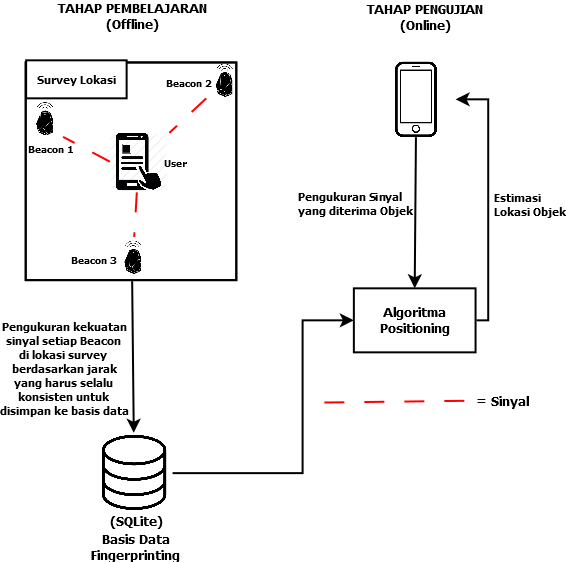
\includegraphics [width = 11cm, height= 9cm]{gambar/fingerprinting}}
\caption{Ilustrasi Metode \textit{Fingerprinting} \citep{Yudha2018}}.
\label{fingerprinting}
\end{figure}

\par Tahap pertama adalah tahap pembelajaran (\textit{offline}), di mana lokasi \textit{Fingerprints} itu sendiri diperoleh dengan cara mengumpulkan RSSI dalam satuan desibel (dBm) yang dipancarkan dari masing-masing AP. Kemudian, gelombang radio akan dipancarkan oleh AP yang diletakkan pada posisi yang telah ditentukan sebelumnya ditangkap oleh \textit{smartphone} dengan kondisi WLAN ataupun Bluetooth dalam keadaan hidup. Selama tahap pembelajaran, lokasi yang tidak diketahui data pembelajarannya kemudian dirujuk sebagai titik referensi estimasi lokasi. 
\newline
\par Tahap kedua adalah tahap pengujian (\textit{online}), di mana keakuratan perkiraan posisi objek sangat bergantung pada jumlah titik referensi yang dikumpulkan dalam data pembelajaran. Selama tahap pengujian, sistem harus memberikan informasi lokasi setiap objek berdasarkan data RSSI yang diamati. Namun, nilai RSSI bisa dipengaruhi oleh keadaan lingkungan sekitar yang dapat mengganggu keakuratannya \citep{Subhan2011}.

\section{\uppercase{RECEIVED SIGNAL STRENGTH INDICATOR (RSSI)}}
\textit{Positioning system} menghasilkan data yang penting untuk menghitung lokasi pengguna. \textit{Time of Arrival} (TOA), \textit{Time Difference of Arrival} (TDOA), \textit{Angle of Arrival} (AOA) dan RSSI adalah metode yang sesuai untuk menghitung data lokasi pengguna untuk kasus \textit{positioning system} \citep{Liu2007}. RSSI menunjukkan kekuatan atau daya yang diterima oleh sinyal \citep{Kajioka2014}. RSSI memperkirakan jarak \textit{node} yang belum diketahui ke referensi node dari beberapa kumpulan unit perhitungan dengan menggunakan atenuasi kekuatan sinyal (\textit{signal strength}) yang dipancarkan dari \textit{transmitter}. Metode ini tepat dilakukan dengan frekuensi sinyal radio \citep{Schneegans2007}.

\par Sebuah nilai RSSI didefinisikan dengan bilangan negatif. Semakin tinggi bilangan negatifnya, maka kekuatan sinyal tersebut tergolong lemah. Namun, jika bilangan nilai RSSI mendekati 0, maka kekuatan sinyal tersebut tergolong kuat. Biasanya, jika suatu objek berada di dekat AP atau \textit{transmitter}, RSSI akan memperoleh nilai yang besar. RSSI dapat digolongkan menjadi 5 kategori kekuatan sinyal seperti terlihat pada Tabel \ref{t_rssi}.

\begin{table}[H]
\centering
\caption{Kekuatan Sinyal RSSI \citep{VerisIndustries2013}}
\label{t_rssi}
\begin{tabular}{|l|l|l|} 
\hline
\textbf{No.} & \textbf{Kekuatan Sinyal} & \textbf{Kualitas Sinyal}  \\ 
\hline
1.           & Kurang dari -40 dB       & Luar Biasa              \\ 
\hline
2.           & -40 dB hingga -55 dB     & Sangat Baik               \\ 
\hline
3.           & -55 dB hingga -70 dB     & Baik                      \\ 
\hline
4.           & -70 dB hingga -80 dB     & Cukup Baik                \\ 
\hline
5.           & Lebih dari -80 dB        & Buruk                     \\
\hline
\end{tabular}
\end{table}

\section{\uppercase{BLUETOOTH LOW ENERGY (BLE)}}
\cite{Keluza2017}, mengemukakan bahwa Bluetooth merupakan alat komunikasi tanpa kabel yang digunakan untuk pertukaran data dalam jarak yang dekat. Bluetooth dikembangkan oleh Ericson di tahun 1994. Kemudian di tahun 1998 Ericson, IBM, Intel, Nokia dan Toshiba membentuk wewenang kekuasaan khusus yang dinamakan dengan Bluetooth Interest Group (SIG). Pertengahan tahun 2010, Bluetooth SIG mengumumkan spesifikasi dari Bluetooth 4.0, yang termasuk di dalamnya meliputi \textit{Bluetooth Classic}, \textit{Bluetooth High Speed} dan BLE. BLE terkadang juga bisa dikatakan sebagai “Bluetooth Pintar”. Meskipun BLE dan \textit{Bluetooth Classic} banyak memiliki kesamaan, BLE sebenarnya memiliki fungsionalitas yang sama sekali berbeda dari \textit{Bluetooth Classic}. 

\par Keunggulan BLE dibandingkan \textit{Bluetooth Classic} adalah konsumsi daya baterai dan energi listrik dari BLE untuk \textit{transfer} data jauh lebih kecil dibandingkan dengan \textit{Bluetooh Classic}, tetapi dengan jangkauan konektivitas dan kapasitas pengiriman data yang sama \citep{bluetoothsig2010}. Karakteristik dari BLE adalah ukurannya yang sangat kecil, biaya murah, serta konsumsi daya rendah yang bisa digunakan sampai beberapa tahun ke depan dengan menggunakan jenis baterai AAA \citep{Keluza2017}. Menurut \cite{Paganini2015}, terdapat beberapa platform yang mendukung BLE dan platfrom tersebut sudah mendukung Bluetooth 4.0. Beberapa platform tersebut adalah sebagai berikut:
\begin {itemize}
\itemsep0em
	\item iOS5+ (lebih dianjurkan iOS7+).
	\item Android 4.3+ (perbaikan \textit{bug} merous di 4.4+).
	\item Apple OS X 10.6+.
	\item Windows 8 (XP, Vista dan Windows 7 hanya mendukung Bluetooth 2.1).
	\item GNU/Linux Vanilla BlueZ 4.93+.
\end{itemize}

\section{\uppercase{BEACON}}
BLE memancarkan sinyal dari alat \textit{transmiter} yang beroperasi menggunakan baterai. Alat \textit{transmiter} tersebut disebut dengan Beacon. Beacon merupakan alat pendeteksi lokasi dengan harga yang terjangkau, ukurannya yang kecil, memiliki daya tahan baterai yang cukup lama, dan tidak membutuhkan energi listrik tambahan. Setiap perangkat \textit{smartphone} dan \textit{tablets} yang mendeteksi sinyal dari Beacon, dapat menghitung jarak dan memperkirakan keberadaan lokasi setiap perangkat sekaligus \citep{Keluza2017}.

\par Kelebihan dari penggunaan Beacon diperkirakan bertahan sampai bertahun-tahun hanya dengan energi baterai, serta tahan terhadap debu dan air sesuai dengan standar IP67, dan memiliki ketelitian sejauh 1-3 meter \citep{Insoft2016}. Teknologi BLE merupakan solusi yang tepat yang digunakan pada Beacon, karena penggunaan dayanya yang murah, BLE juga termasuk sistem yang ramah lingkungan. Penggunaan daya yang murah pada BLE dicapai dengan menjaga waktu proses transmisi data sesingkat mungkin dan mengizinkan perangkat \textit{smartphone} maupun \textit{tablets} berada pada mode tidur saat proses transmisi data \citep{Lindh2015}.

\section{\uppercase{Metode K-NEAREST NEIGHBOR (K-NN)}}
K-NN merupakan salah satu metode klasifikasi yang sederhana. Metode klasifikasi K-NN telah diterapkan sejak tahun 1970 dalam perkiraan statistik dan pengenalan pola \citep{Park2015}. K-NN merupakan salah satu metode klasifikasi menggunakan pendekatan \textit{supervised-learning} sehingga membutuhkan data pembelajaran yang sudah dilabeli \citep{LukitoAntonius2015}. Berdasarkan data pembelajaran tersebut, satu titik dapat diklasifikasikan dengan cara menghitung jarak terdekat dengan \textit{k}-tetangga terdekat di \textit{class} sekitarnya \citep{Kadyan2016}. Setiap data pembelajaran tersebut akan direpresentasikan sebagai sebuah titik pada ruang dimensi \textit{n}. K-NN akan mencari ruang dan pola untuk \textit{k}-tetangga terdekat yang paling dekat dengan data tersebut saat data kelas yang diberikan tidak diketahui \citep{Imandoust2013}.

\begin{figure}[H]
	\centering
	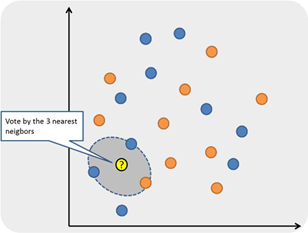
\includegraphics [width = 7cm, height= 5.5cm]{gambar/knn}
	\caption{Ilustrasi Contoh K-NN dengan Nilai \textit{k}=3 \citep{suryanto2016}}.
	\label{knn}
\end{figure}

\par Pada Gambar \ref{knn} terlihat bahwa penentuan kelas dari data baru berdasarkan data pembelajaran dengan ruang 2 dimensi sebagai contoh K-NN dengan nilai \textit{k}=3. Jarak antara data baru dengan data pembelajaran biasanya dihitung berdasarkan fungsi jarak yang umum digunakan yaitu \textit{Euclidean Distance}. Jika terdapat data $P1 = (p_{11}, p_{12},...., p_{1n})$ dan $P2 = (p_{21}, p_{22},...., p_{2n})$ dimana $n$ merupakan jumlah Beacon yang digunakan, maka perhitungan jarak dengan rumus \textit{Euclidean Distance} adalah sebagai berikut:
\begin{equation}
d(P1,P2)=\sqrt{\sum_{i=1}^{n}(p_{1i}-p_{2i})^2}
\end{equation}

\par Algoritma K-NN dikatakan sebagai \textit{nearest neighbor} apabila terdapat kasus khusus yaitu di mana klasifikasi diprediksikan berdasarkan data pembelajaran yang paling dekat (dengan kata lain, nilai \textit{k}=1) \citep{sutarti2016}. Nilai \textit{k} yang terbaik untuk algoritma K-NN bergantung pada banyaknya data. Namun, secara umum nilai \textit{k} yang memiliki nilai sebesar 1 atau 2 memberikan hasil yang terbaik. Nilai \textit{k} yang tinggi akan membuat batasan antara setiap klasifikasi menjadi lebih kabur \citep{otsason2005}.

\section{\uppercase{ANDROID}}
Android adalah sistem operasi untuk perangkat \textit{smartphone} berbasis Linux \citep{Safaat2011}. Android menyediakan platform \textit{open source} bagi para \textit{developer} untuk menciptakan aplikasi mereka sendiri untuk digunakan oleh bermacam peranti bergerak. Aplikasi Android di tulis dengan bahasa pemrograman Java. Bagaimanapun juga, tanpa menggunakan standar Java Virtual Machine (JVM) sebuah aplikasi Android tidak akan bisa berjalan. Android SDK menyediakan sebuah \textit{tools} dan API untuk mengembangkan sebuah aplikasi pada platform \citep{Golhar2016}. Menurut \cite{Supardi2011}, ada 4 komponen utama pada aplikasi Android yaitu sebagai berikut:
\begin{enumerate}[1.]
\itemsep0em
\item \emph{Activities}, merupakan komponen untuk menyajikan tampilan aplikasi kepada pengguna (\textit{user interface}).
\item \emph{Service}, merupakan komponen yang tidak memiliki \textit{user interface} atau disebut dengan \textit{layout} pada Android. Namun, \textit{service} ini bekerja dengan cara \textit{background processing}.
\item \emph{Broadcast Receiver}, merupakan komponen yang berfungsi menerima dan bertugas untuk menyampaikan notifikasi.
\item \emph{Content Provider}, merupakan komponen yang menangani data secara spesifik sehingga dapat digunakan oleh aplikasi lain.
\end{enumerate}

\section{\uppercase{ANDROID STUDIO}}
Android Studio merupakan \textit{Integrated Development Environtment} (IDE) untuk pengembangan platform Android. Android Studio dapat digunakan secara gratis di bawah pengawas Apache License 2.0. Android Studio pertama kali diperlihatkan dimulai dari versi 0.1 pada bulan Mei 2013, kemudian memasuki tahap Beta dimulai dari versi 8.0 yang dirilis pada bulan Juni 2014. Pertama kali dibangun secara stabil pada bulan Desember 2014, dimulai dengan versi 1.0 dikembangkan berdasarkan Jet Brains IntelliJ IDEA \textit{software} dan Android Studio didesain untuk \textit{developer} Android \citep{Singh2016}.

\section{\uppercase{WEB SERVICES}}
\textit{Web services} menggambarkan aplikasi yang mengekspos \textit{business logic} sebagai layanan yang menggunakan internet \citep{Mironela2009}. Layanan tersebut dikirim melalui \textit{interface} yang dapat diprogram, sementara fungsionalitasnya dapat dipakai dan dipanggil melalui alamat \textit{Internet Protocol} (IP \textit{address}) \citep{Wagh2012}. \textit{Web services} sering dikategorikan sebagai komponen sistem perangkat lunak yang dirancang untuk mendukung interaksi antar sistem. \textit{Web services} menyediakan informasi atau data kepada sistem lain untuk digunakan sebagai fasilitas yang membuat sistem dapat saling berinteraksi. Biasanya, data yang diberikan oleh \textit{web services} berupa data dalam bentuk format JavaScript Object Notation (JSON) atau eXtensible Markup Language (XML) \citep{Rahman2013}. Situs \textit{web} World Wide Web Consortium (W3C) mendeskripsikan  bahwa \textit{Simple Object Access Protocol} (SOAP), \textit{REpresentatonal State Transfer} (REST) merupakan protokol yang digunakan \textit{web services} untuk berkomunikasi. Penelitian ini akan menggunakan \textit{web services} dengan layanan protokol REST untuk membantu aplikasi absensi perkuliahan berbasis Android berinteraksi dengan \textit{database} yang terdapat di server.

\section{\uppercase{REpPRESENTATIONAL STATE TRANSFER (REST)}}
REST merupakan hubungan antara klien dan server dan bagaimana sebuah data disimpan. Arsitektur REST didasarkan pada gaya arsitektur klien atau server yang dapat dilihat pada Gambar \ref{restful}. \textit{Request} dan \textit{response} dibangun berdasarkan sumber daya pada saat proses transfer \citep{HaliliRamadani2018}. Konsep dari REST adalah perpindahan antar \textit{state}, dapat dicontohkan seperti sebuah browser yang melakukan permintaan terhadap sebuah halaman situs, maka server akan mengirimkan \textit{state} dari halaman situs tersebut ke browser \citep{Rahman2013}.
\begin{figure}[H]
	\centering
	\shadowbox
	{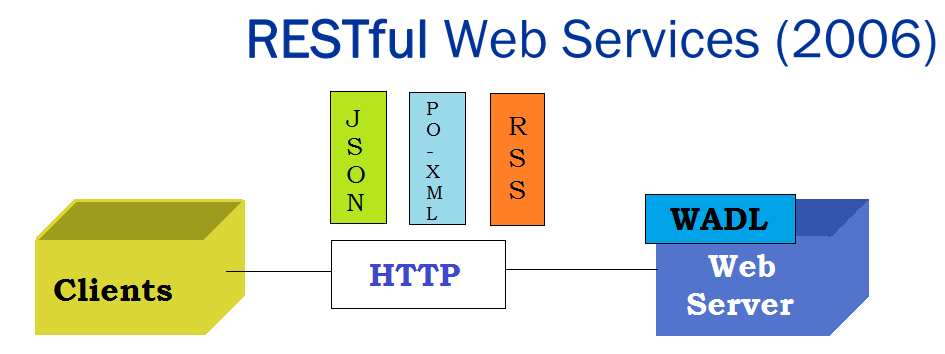
\includegraphics [width = 11cm, height= 3cm]{gambar/restful}}
	\caption
	{Ilustrasi Arsitektur RESTful dan Komunikasi Antara Klien dan Server \citep{HaliliRamadani2018}}.
	\label{restful}
\end{figure}
\par Navigasi REST dilakukan melalui HTTP untuk melakukan aktivitas tertentu, seolah-olah terjadi perpindahan \textit{state} antara satu halaman dengan halaman lainnya \citep{Rahman2013}. Sebuah aplikasi \textit{web} yang bergantung dengan layanan REST arsitektur disebut dengan RESTful \textit{web services}. RESTful \textit{web services} menggunakan 4 perintah HTTP untuk \textit{create}, \textit{read}, \textit{update} dan \textit{delete} yaitu \textit{GET}, \textit{POST}, \textit{PUT} dan \textit{DELETE} seperti yang terlihat pada Gambar \ref{httprestful} \citep{sinha2014}.
\begin{figure}[H]
	\centering
	\shadowbox
	{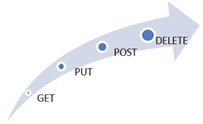
\includegraphics [width = 5cm, height= 3cm]{gambar/httprestful}}
	\caption{Perintah HTTP RESTful \citep{sinha2014}}.
	\label{httprestful}
\end{figure}

\section{\uppercase{SCRUM}}
\textit{Scrum} pada dasarnya didasari oleh proses model \textit{Incremental} yang merupakan salah satu model pengembangan perangkat lunak. Dalam metode \textit{Scrum}, seluruh \textit{development cycle} terbagi menjadi sebuah rangkaian iterasi di mana setiap iterasi tersebut merupakan detak jantung dari \textit{Scrum} itu sendiri yang disebut dengan “\textit{Sprint}”. Pengerjaan \textit{Sprint} memiliki durasi maksimal selama 30 hari. Karena durasi \textit{Sprint} lebih singkat dibandingkan dengan durasi pengembangan produk, maka dalam produk \textit{development cycle} akan ada beberapa \textit{Sprint}, yang artinya pengembangan produk dengan metode \textit{Scrum} dilakukan secara \textit{Iterative} dan \textit{Incremental}. Tahapan-tahapan metode \textit{Scrum} menurut \cite{Schwab2013} adalah sebagai berikut:
\begin {enumerate}[1.]
\item Dimulai dengan mengumpulkan \textit{user requirements}, namun tidak harus semua \textit{requirements} diharapkan harus keluar dari pemikiran \textit{user} di tahap awal proses pengembangan. \textit{User} dapat mengubah pikiran mereka di setiap waktu selama proses pengembangan, \textit{user} dapat menambah fitur-fitur baru, menghapus atau memperbarui beberapa fitur yang telah ada sebelumnya. 
%%%%%%%%%%%%%%%%%%%%%%%%%%%%%%%%%%%%%%%%%%%%%%%%%%%%%%%%%%%%%%%%%%%%%%%%%%%%%%%%%%%%%%%%%%%%%%%%%%%%%%%%%
\item Tahapan selanjutnya adalah memprioritaskan \textit{requirements} dan \textit{Product Backlog}. Sebuah perencanaan yang tepat dalam \textit{Sprint} harus dilakukan sesuai jumlah \textit{Sprint} yang dibutuhkan untuk mengembangkan perangkat lunak, yang terdiri dari durasi \textit{Sprint} tersebut dan \textit{requirements} apa saja yang terdapat di \textit{Product Backlog} yang harus diimplementasikan di setiap \textit{Sprint} (dikenal dengan \textit{Sprint Backlog}). 
%%%%%%%%%%%%%%%%%%%%%%%%%%%%%%%%%%%%%%%%%%%%%%%%%%%%%%%%%%%%%%%%%%%%%%%%%%%%%%%%%%%%%%%%%%%%%%%%%%%%%%%%%
\item \textit{Sprint} diawali dengan \textit{Sprint Planning} dimana \textit{Product Owner}, satu orang yang telah diberikan wewenang dan bertanggung jawab untuk memaksimalkan nilai produk di pasar, bertemu dengan tim \textit{Scrum} (tim dengan jumlah 2-9 orang), kemudian bekerja sama untuk memperkirakan \textit{requirements} dari \textit{Product Backlog} apa saja yang dikerjakan selama satu \textit{Sprint}.
%%%%%%%%%%%%%%%%%%%%%%%%%%%%%%%%%%%%%%%%%%%%%%%%%%%%%%%%%%%%%%%%%%%%%%%%%%%%%%%%%%%%%%%%%%%%%%%%%%%%%%%%% 
\item \textit{Sprint Planning} difasilitasi dengan \textit{Scrum Master}. \textit{Scrum Master} adalah seorang pemimpin yang melayani (\textit{Servant Leader}). \textit{Sprint Planning} memiliki batasan waktu selama 8 jam di dalam sebuah \textit{Sprint} yang berdurasi selama 30 hari. Keluaran dari \textit{Sprint Planning} adalah daftar pekerjaan dari hasil kesepakatan antara \textit{Product Owner} dan tim \textit{Scrum} dimana pekerjaan itu yang akan dikerjakan oleh tim \textit{Scrum} nantinya selama satu \textit{Sprint} beserta \textit{Sprint Goal} yang dinamakan dengan \textit{Sprint Backlog}. 
%%%%%%%%%%%%%%%%%%%%%%%%%%%%%%%%%%%%%%%%%%%%%%%%%%%%%%%%%%%%%%%%%%%%%%%%%%%%%%%%%%%%%%%%%%%%%%%%%%%%%%%%%
\item Setelah \textit{Sprint Planning} berakhir, tim \textit{Scrum} akan mengambil \textit{Sprint Backlog} untuk diri mereka masing-masing dan mengerjakan \textit{Sprint Backlog} setiap hari hingga akhir \textit{Sprint} tanpa campur tangan dari pihak manapun. \textit{Daily Scrum} akan dikerjakan oleh tim \textit{Scrum} yang tidak lebih dari 15 menit untuk menentukan apa saja yang akan mereka kerjakan selama 24 jam ke depan berdasarkan perkembangan 24 jam terakhir, serta menyampaikan permasalahan yang menghambat mereka untuk bisa mencapai \textit{Sprint Goal}. Tim \textit{Scrum} akan melakukan perbaikan-perbaikan item dari \textit{Product Backlog} pada \textit{Sprint} yang akan datang selama proses pengembangan berlangsung, dengan tujuan membuat \textit{Sprint Planning} menjadi lebih efektif.
%%%%%%%%%%%%%%%%%%%%%%%%%%%%%%%%%%%%%%%%%%%%%%%%%%%%%%%%%%%%%%%%%%%%%%%%%%%%%%%%%%%%%%%%%%%%%%%%%%%%%%%%%
\item Di akhir \textit{Sprint} saat acara \textit{Sprint Review}, \textit{Product Owner} akan mempresentasikan hasil pekerjaan tim \textit{Scrum} selama satu \textit{Sprint} dan juga menjelaskan apa saja pencapaian tim \textit{Scrum} menuju \textit{Sprint Goal} di dalam \textit{Sprint} tersebut kepada para pemegang kepentingan (\textit{stakeholder}) agar mendapatkan \textit{feedback}. \textit{Feedback} ini akan dimasukkan ke dalam \textit{Product Backlog} agar meningkatkan nilai dari sebuah produk. \textit{Sprint Review} memiliki batasan waktu tidak lebih dari 4 jam untuk \textit{Sprint} yang memiliki durasi selama 30 hari.
%%%%%%%%%%%%%%%%%%%%%%%%%%%%%%%%%%%%%%%%%%%%%%%%%%%%%%%%%%%%%%%%%%%%%%%%%%%%%%%%%%%%%%%%%%%%%%%%%%%%%%%%%
\item Setelah \textit{Sprint Review}, \textit{Scrum Master} memfasilitasi acara yang bernama \textit{Sprint Retrospectives} agar tim \textit{Scrum}, \textit{Product Owner} bekerja sama menentukan apa saja peningkatan yang akan mereka implementasikan di \textit{Sprint} berikutnya. \textit{Scrum Master} yang efektif, akan kreatif dalam memfasilitasi \textit{Sprint Retrospectives}, akan masuk ke dalam \textit{Sprint Backlog} untuk menuju \textit{Sprint} berikutnya. \textit{Definition of Done} adalah salah satu hal yang ditekankan oleh tim \textit{Scrum} pada saat \textit{Sprint Retrospectives}.
%%%%%%%%%%%%%%%%%%%%%%%%%%%%%%%%%%%%%%%%%%%%%%%%%%%%%%%%%%%%%%%%%%%%%%%%%%%%%%%%%%%%%%%%%%%%%%%%%%%%%%%%%
\item \textit{Sprint Retrospectives} merupakan acara yang paling penting dalam \textit{Scrum} dikarenakan sifatnya yang menekankan \textit{continuous learning} yang dapat meningkatkan tingkat \textit{agility} perusahaan. \textit{Sprint Review} memiliki batasan waktu tidak lebih dari 3 jam untuk \textit{Sprint} yang memiliki durasi selama 30 hari. Setelah \textit{Sprint Retrospectives} berakhir, maka \textit{Sprint} berikutnya akan langsung dilakukan tanpa ada jeda antar \textit{Sprint}. Pada setiap \textit{Sprint}, \textit{Product Owner} akan memastikan agar produk dapat mencapai nilai setinggi mungkin saat pengembangan produk diakhiri. \textit{Product Owner}, \textit{Scrum Master} dan tim \textit{Scrum} memegang komitmen, keberanian, saling menghargai satu sama lain, keterbukaan dan fokus. Ilustrasi tahapan-tahapan metode Scrum dapat dilihat pada Gambar \ref{scrum} dibawah ini.
\end{enumerate} 

\vspace{0,2cm}
\begin{figure}[H]
	\centering
	\shadowbox
	{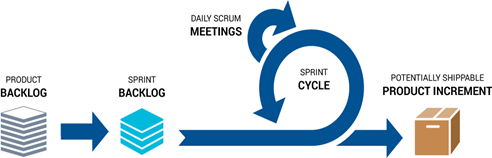
\includegraphics [width = 11cm, height= 3.5cm]{gambar/scrum}}
	\caption{Ilustrasi Metode Pengembangan Menggunakan \textit{Scrum} \citep{Schwab2013}}.
	\label{scrum}
\end{figure}


\section{\uppercase{BLACK BOX TESTING}}
\textit{Black box testing} merupakan pengujian yang hanya dilakukan dengan mengeksekusi dan menjalankan aplikasi itu sendiri untuk mengamati apakah prosesnya sesuai dengan bisnis yang diinginkan \citep{Alfatta2007}. \textit{Black box testing} berfokus pada spesifikasi fungsionalitas perangkat lunak. \textit{Black box testing} menurut \citep{Mustaqbal2015} cenderung menemukan hal-hal berikut:
\begin{enumerate}[1.]
\item Fungsi yang tidak benar atau tidak ada.
\item Kesalahan \textit{user interface}.
\item Kesalahan pada struktur data dan akses \textit{database}.
\item Kesalahan performansi.
\item Kesalahan inisialisasi dan terminasi.
\end{enumerate}

\section{\uppercase{USABILITY TESTING}}
\textit{Usability testing} adalah kegiatan pengujian untuk mengumpulkan data mengenai sebuah produk dalam tahap pengembangan. Tujuan utama dari \textit{usability testing} adalah untuk mengumpulkan data kuantitatif dengan mengukur waktu untuk mempelajarinya, performa kecepatan dan tingkat \textit{human error} \citep{Wahl2000}. \textit{Usability testing} ini dilakukan dengan cara mendudukkan pengguna di pusat, kemudian mengambil pelajaran dari sana. Pengujian ini diharapkan akan mendapatkan kekuatan dan kelemahan dari setiap aspek yang ada pada aplikasi itu sendiri. Maka dari itu, perlu adanya dokumentasi pengalaman aktual para calon pengguna aplikasi atau produk saat dievaluasi \citep{Wesfix2017}.

\par Tujuan lain dilakukannya pengujian ini adalah untuk mengumpulkan data kualitatif yang berhubungan dengan kepuasan pengguna dengan produk yang diuji. Data kualitatif tersebut terdiri dari komentar yang dibuat oleh partisipan, jawaban dari kuisioner pertanyaan dan tanggapan dari partisipan saat proses wawancara. \textit{Usability testing} telah terbukti dapat mengurangi waktu tahap pengembangan, mengurangi jumlah \textit{bugs}, dan menghasilkan produk yang lebih berkualitas untuk meningkatkan nilai jual \citep{Wahl2000}.

\subsection{System Usablity Scale (SUS)}
Metode pengujian dengan \textit{usablity testing} yang digunakan pada penelitian ini adalah SUS. Pada tahun 1996, John Broke menerbitkan sebuah makalah tentang “\textit{quick and dirty}” unidimensional \textit{usability scale} yang dinamakan dengan \textit{System Usablity Scale} (SUS). SUS dikembangkan sebagai sebuah tanggapan dengan biaya yang murah dan praktis yang berfungsi untuk analisis kegunaan aplikasi/produk. Metode pengujian SUS merupakan pengujian untuk mendapatkan penilaian subjektif dari sudut pandang pengguna \citep{Brooke1996}.

\par Skala penilaian yang digunakan yaitu skala likert antara 1-5. \cite{Sugiyono2004} mengatakan bahwa skala likert digunakan untuk mengukur pendapat, persepsi dan sikap seseorang atau sekelompok orang tentang fenomena sosial. SUS bertujuan untuk mengetahui penilaian subjektif yang dilakukan dalam pengujian oleh beberapa responden dan meminta pendapat mengenai aplikasi yang akan dibuat pada penelitian ini.
\par Pengujian ini memerlukan kuesioner sebagai teknik pengumpulan informasi pengujian yang didapat dari responden mengenai aplikasi. Kuesioner terdiri dari 10 soal yang terdiri dari pertanyaan positif dan negatif. Pertanyaan positif terdapat pada nomor ganjil (1, 3, 5, 7, 9) dan pertanyaan negatif terdapat pada nomor genap (2, 4, 6, 8, 10). Setiap pertanyaan diberi bobot antara 0-4. Pertanyaan ganjil skor dihitung dengan cara bobot tiap pertanyaan ($x_{i}$) dikurangi 1 (ditulis $x_{i}$ - 1). Sedangkan pertanyaan genap skor dihitung dengan cara 5 dikurangi bobot tiap pertanyaan ($x_{i}$)(ditulis 5 - $x_{i}$) \citep{Ardiansyah2016}. Setiap pertanyaan memiliki 5 pilihan jawaban yang terdiri dari: sangat tidak setuju, tidak setuju, biasa saja, setuju dan sangat setuju.

%\par Rumus menghitung skor pengujian \textit{usability testing} adalah sebagai berikut:
%\begin{equation}
%\overline{x}=\frac{\sum x}{n}
%\end{equation}
%\newline
%Keterangan:\newline
%$\overline{x}$ = skor rata-rata. \newline
%$\sum x$ = jumlah skor SUS. \newline
%$n$ = jumlah responden. 

\subsection{Test Plan}
\textit{Test plan} adalah dokumen yang melibatkan semua anggota tim \textit{developer} untuk melihat apakah fungsionalitas dari produk yang dibuat sudah terpenuhi atau belum. Dengan kata lain, \textit{test plan} disebut sebagai tujuan, perencanaan atau skenario untuk melakukan \textit{testing} yang akan dilakukan baik itu \textit{expert} \textit{user} atau \textit{user} awam. \textit{Test plan} perlu dibuat saat melakukan pengujian karena \textit{test plan} menggambarkan bagaimana cara menguji produk tersebut. \textit{Test plan} memaksa untuk melakukan pengujian secara sistematis \citep{Rubin2008}. Bagian-bagian dari \textit{test plan} menurut \cite{Rubin2008} adalah sebagai berikut:
\begin{itemize}
\item Maksud, tujuan dan sasaran pengujian.
\item Pertanyaan terkait penelitian.
\item Karakteristik partisipan.
\item Metode yang digunakan (\textit{test design}).
\item \textit{List} tugas.
\item Lingkungan pengujian, perlengkapan, dan logistik.
\item Peran moderator pengujian.
\item Data yang dikumpulkan dan langkah-langkah evaluasi.
\item Laporan dan presentasi.
\end{itemize}








%-----------------------------------------------------------------------------%

% Baris ini digunakan untuk membantu dalam melakukan sitasi
% Karena diapit dengan comment, maka baris ini akan diabaikan
% oleh compiler LaTeX.
\begin{comment}
\bibliography{daftar-pustaka}
\end{comment}


	%-------------------------------------------------------------------------------
%                            BAB III
%               		METODOLOGI PENELITIAN
%-------------------------------------------------------------------------------
\fancyhf{} 
\fancyfoot[C]{\thepage}
\chapter{METODOLOGI PENELITIAN}

\section{\uppercase{WAKTU DAN LOKASI PENELITIAN}}
\setlength\parindent{30pt} Penelitian ini dilaksanakan di Ruang Kuliah B.03.02 yang terletak di lantai 3 Blok B dan Ruang Kuliah E.02.07 yang terletak di lantai 2 Blok E, Gedung FMIPA Universitas Syiah Kuala (Unsyiah). Waktu yang dibutuhkan untuk penelitian ini adalah 6 bulan terhitung dari bulan Juli 2019 hingga Februari 2020. 

\section{\uppercase{ALAT DAN BAHAN}}
Alat dan bahan yang digunakan pada penelitian ini meliputi perangkat keras, perangkat lunak dan bahan yang mendukung pada penelitian ini adalah data \textit{Received Signal Strength Indicator} (RSSI) dari hasil survei di lokasi penelitian. Perangkat lunak yang digunakan adalah:
\begin{itemize}
\itemsep0em
\item OS Windows 10.
\item Android Studio 3.6.
\item IntelliJ IDEA 2019.3.3.
\item PhpStorm 2019.3.3.
\item Postman 7.19.1.
\end{itemize}

\par Sedangkan komponen perangkat keras yang digunakan meliputi 1 unit Laptop Lenovo dengan RAM 6GB, Intel® Core™ i5-3230M CPU @2.60Ghz (4 CPUs), ~2.6 GHz Processor, \textit{Harddisk} 500GB, \textit{Solid State Drive} (SSD) 120GB, memiliki Sistem Operasi Windows 64-bit, 3 unit Nyvida Beacon, dan 6 unit FeasyBeacon. 

\section{\uppercase{METODE PENELITIAN}}
Metode penelitian yang dilakukan terdiri dari beberapa tahapan. Skema dari alur tahapan tersebut dapat dilihat pada Gambar \ref{metpen}.
\begin{figure}[H]
\centering
{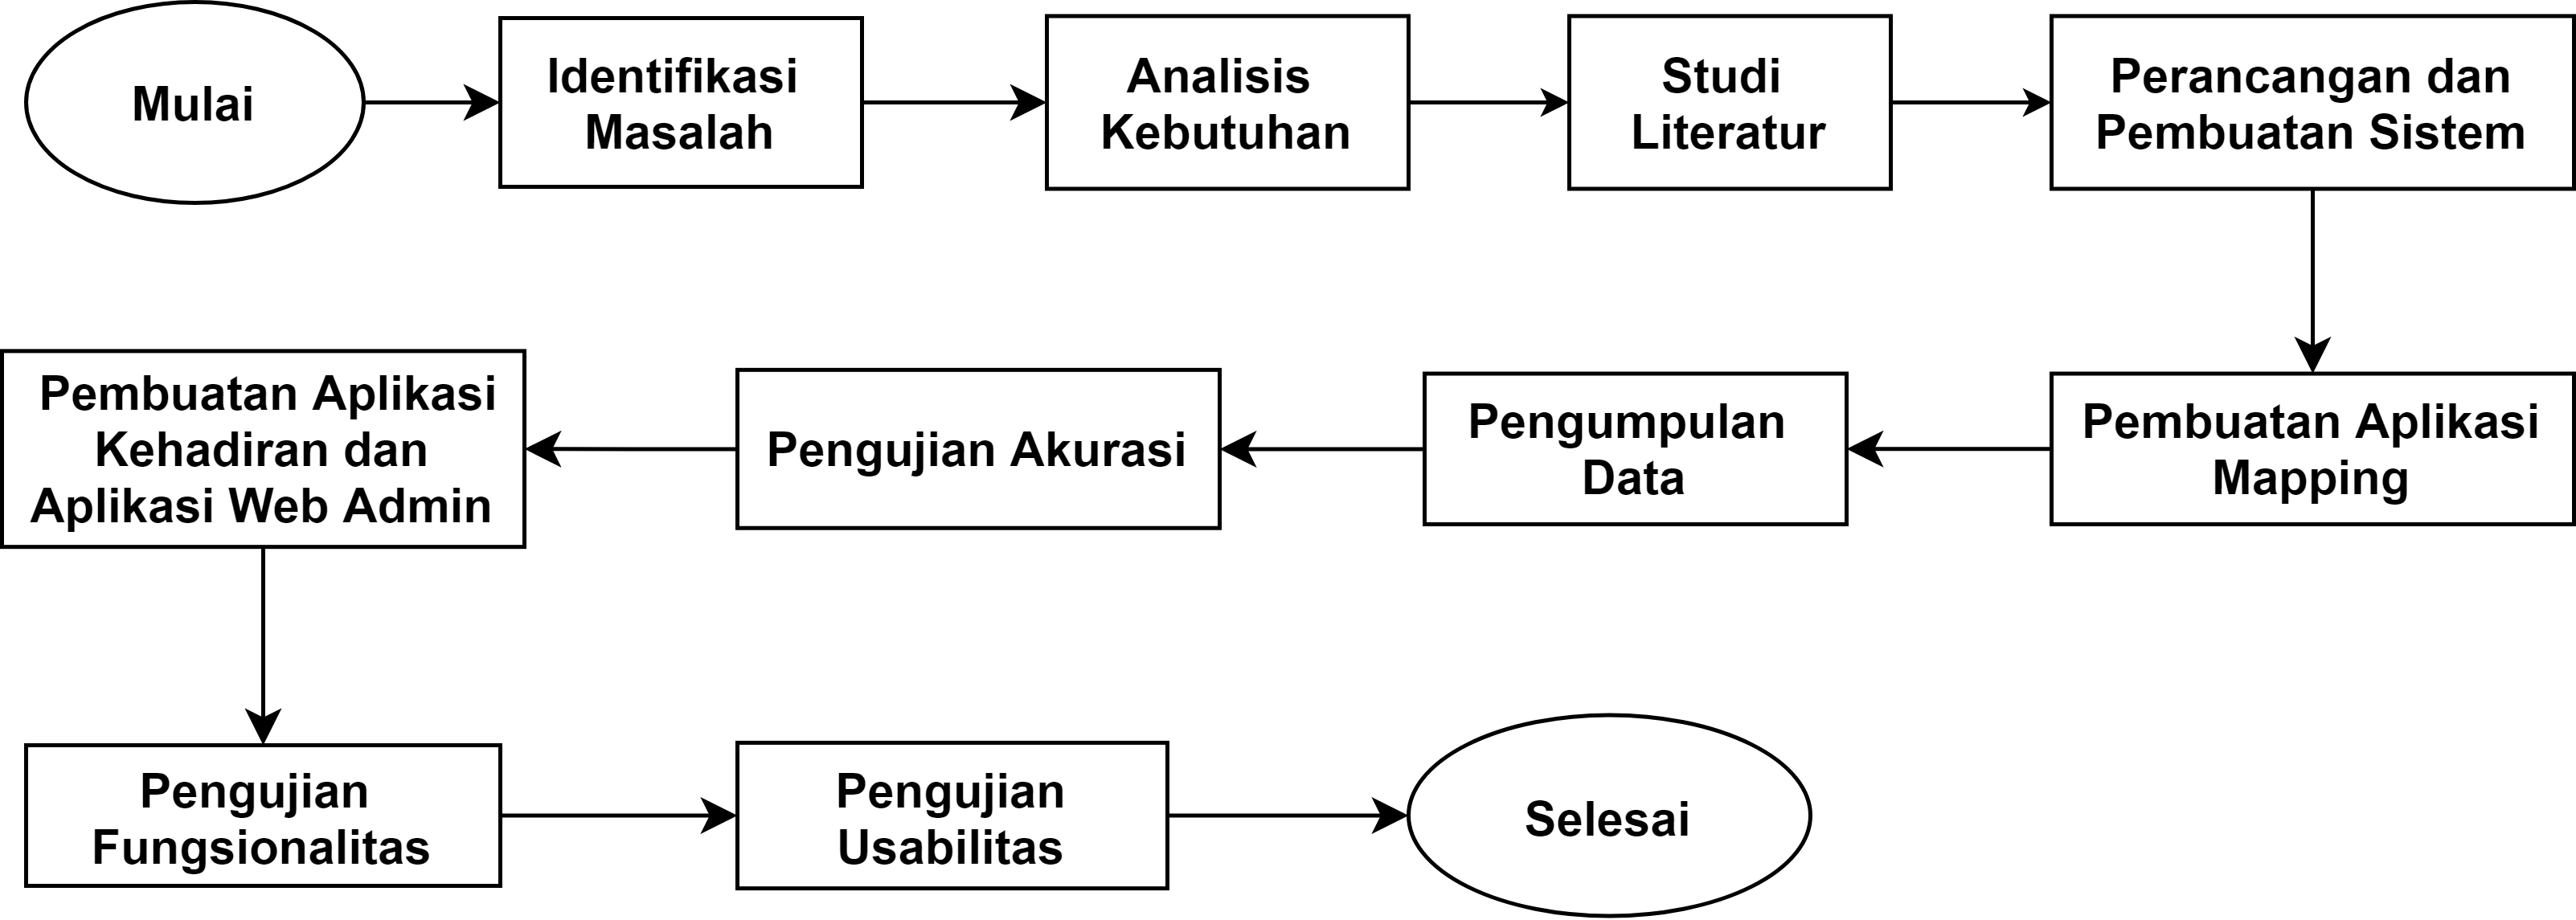
\includegraphics [width = 14cm, height= 6cm]{gambar/diagram-alir-penelitian}}
\caption{Diagram Alir Penelitian}
\label{metpen}
\end{figure}

\fancyhf{} 
\fancyfoot[R]{\thepage}

\subsection{Identifikasi Masalah}
Tahapan ini merupakan tahapan yang dilakukan untuk mengidentifikasi masalah sehingga aplikasi ini perlu dibuat. Masalah-masalah yang berhasil diidentifikasi adalah sebagai berikut:
\begin{enumerate}[1.]
\itemsep0em
\item Belum tersedia Aplikasi Mapping untuk pemetaan kekuatan sinyal atau pemetaan nilai RSSI berbasis Android. 
\item Teknologi GPS tidak berfungsi dengan baik apabila digunakan di dalam gedung \citep{Keluza2017}.
\item Belum tersedia Aplikasi Kehadiran berbasis Android di Jurusan Informatika Unsyiah.
\end{enumerate}

%%%%%%%%%%%%%%%%%%%%%%%%%%%%%%%%%%%%%%%%%%%
\subsection{Analisis Kebutuhan}
Tahapan ini dilakukan untuk mengetahui kebutuhan yang bersumber dari masalah yang telah diidentifikasi sebelumnya sehingga perancangan aplikasi dibangun sesuai kebutuhan. Kebutuhan dari sistem yang dibangun adalah sebagai berikut:

\par \textbf{Kebutuhan Fungsional} Kebutuhan fungsional mendefinisikan fungsionalitas sistem. Kebutuhan fungsional dari identifikasi masalah yang telah dilakukan adalah sebagai berikut:

\begin{itemize}
\item Melakukan proses pencatatan kehadiran dosen dan mahasiswa secara \textit{background proccess} dengan aplikasi berbasis Android dengan akurasi yang baik apabila di dalam gedung.

\item Menampilkan prediksi lokasi pengguna.

\end{itemize}

\par \textbf{Kebutuhan Non-Fungsional} Kebutuhan non-fungsional memastikan batasan eksternal yang harus dipenuhi oleh sistem. Batasan-batasan tersebut antara lain:
\begin{itemize}
\item Proses pencatatan kehadiran perkuliahan dimulai oleh dosen.

\item Dosen dan mahasiswa tidak dapat melakukan proses pencatatan kehadiran apabila terlambat 50 menit sebelum perkuliahan berakhir.

\item Proses pencatatan kehadiran dilakukan secara \textit{background proccess} dengan menit yang diacak setiap rentang waktu 10 menit.

\item Hanya dapat melakukan proses pencatatan kehadiran apabila Bluetooth pada perangkat hidup dan terkoneksi dengan internet.

\item Sistem hanya dapat mendeteksi lokasi pengguna di dalam gedung yang telah dipetakan terlebih dahulu.
 
\end{itemize}

%%%%%%%%%%%%%%%%%%%%%%%%%%%%%%%%%%%%%%%%%
\subsection{Studi Literatur}
Studi literatur digunakan sebagai bahan referensi selama proses penelitian. Studi literatur dilakukan dengan cara mencari situs \textit{website} dan jurnal-jurnal terkait tentang penelitian, baik jurnal nasional maupun jurnal internasional, buku-buku yang telah diterbitkan, serta situs-situs internet yang berkaitan dengan permasalahan yang dikaji dalam penelitian. Studi literatur dapat dikembangkan untuk menyempurnakan kekurangan dari penelitian sebelumnya. 

\subsection{Perancangan Sistem dan Pembuatan Sistem}
\subsection{Perancangan Sistem}
Tahap perancangan sistem ini meliputi perancangan alur kerja sistem yang berfungsi untuk memastikan sistem yang dibangun dapat digunakan secara baik oleh pengguna. Alur kerja dari sistem yang dibangun dijelaskan dengan menggunakan diagram alir yang dapat dilihat pada Gambar \ref{alur-kerja-sistem}.

\begin{figure}[H]
\centering
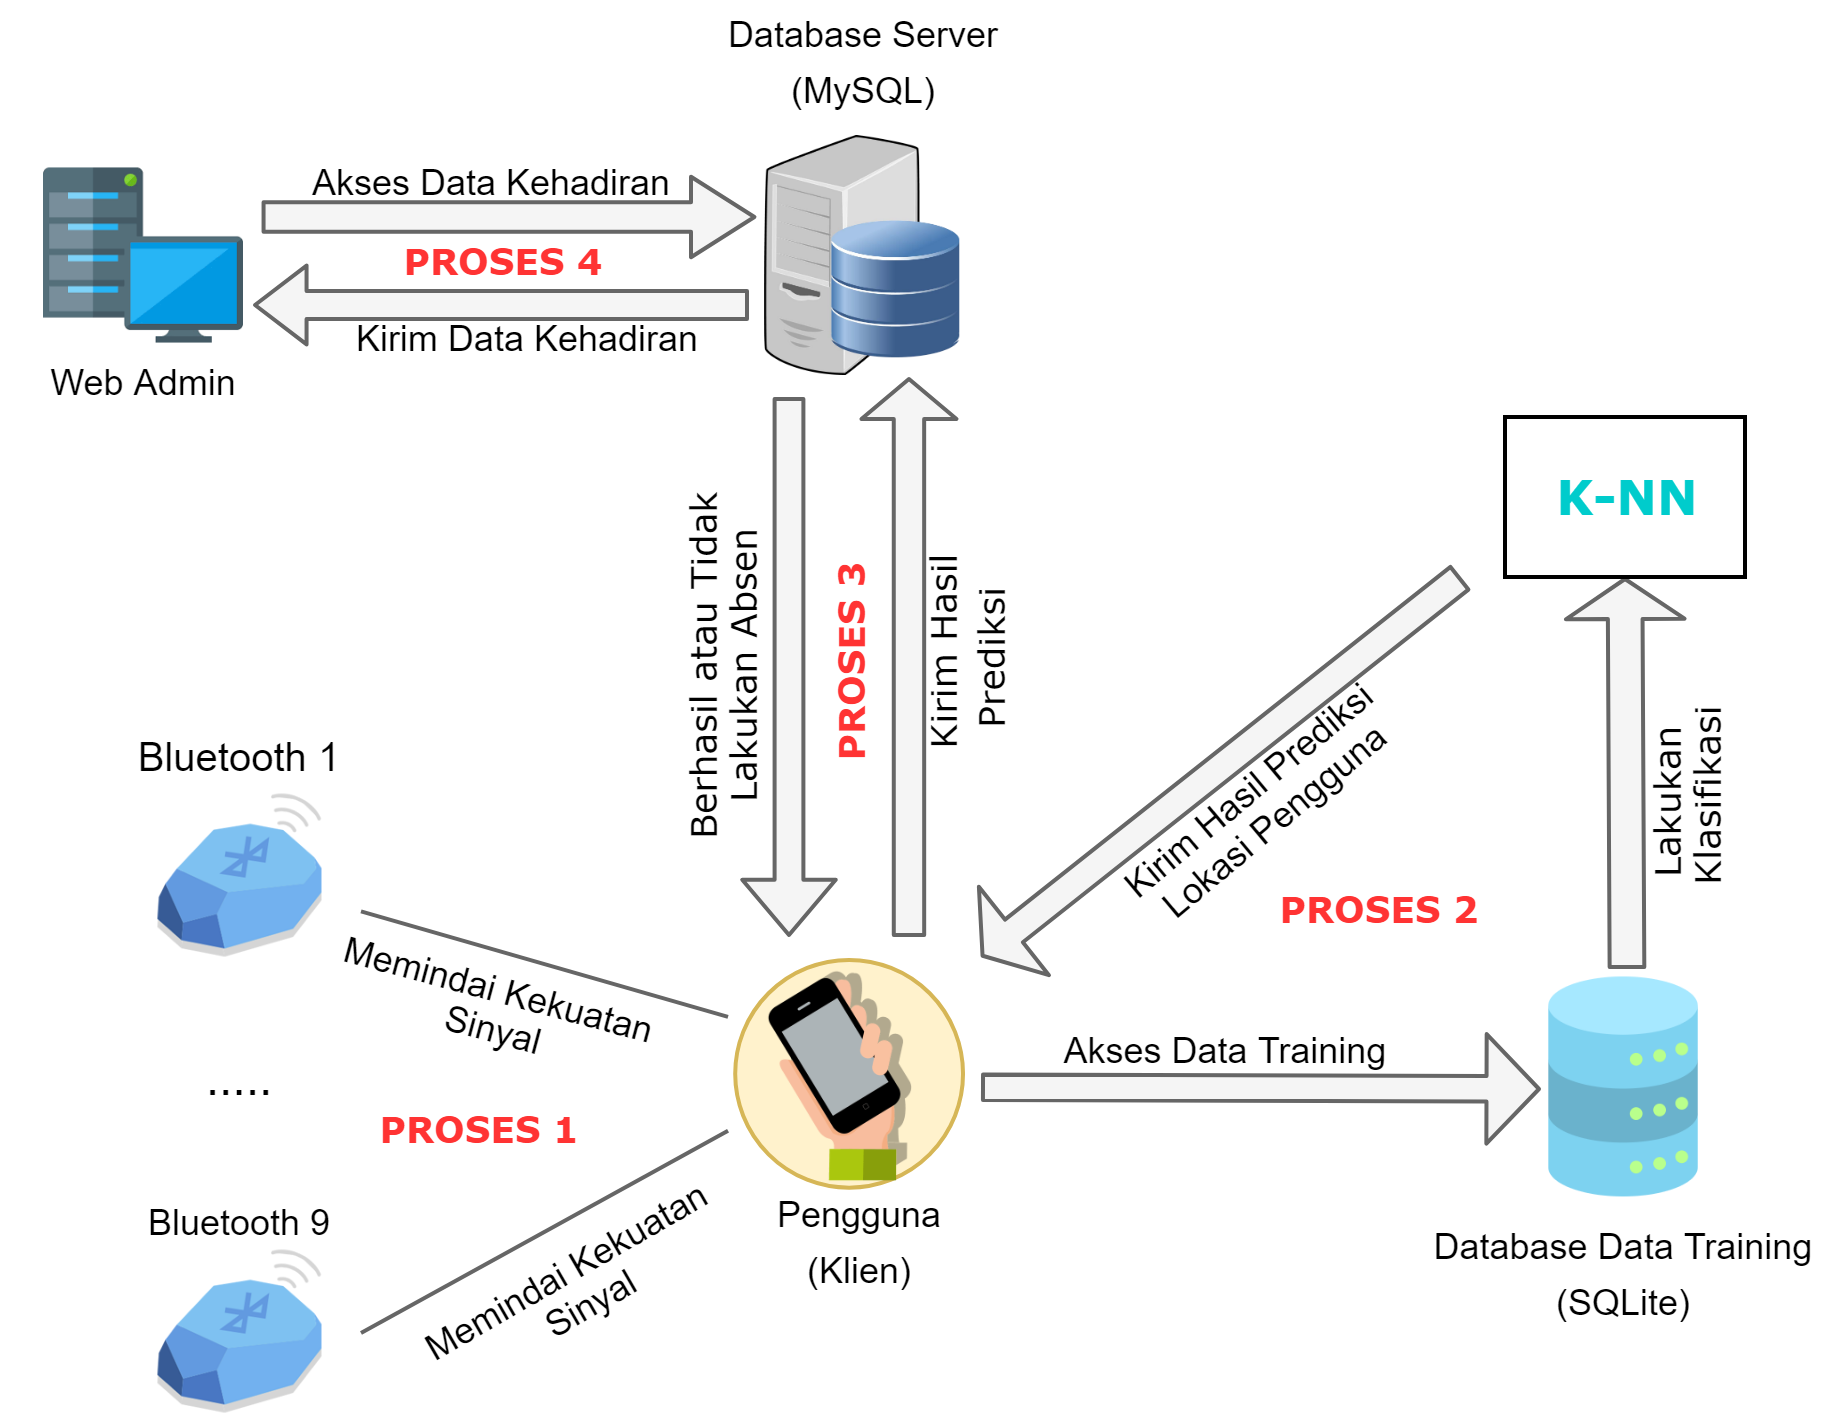
\includegraphics[width=10cm, height=8cm]{gambar/alur-kerja-aplikasi}
\caption{Alur Kerja Sistem.}
\label{alur-kerja-sistem}
\end{figure}

\subsection{Pembuatan Sistem}
Pada proses pembuatan sistem, metode pengembangan perangkat lunak yang digunakan yaitu metode \textit{Scrum}, dikarenakan sistem ini dikembangkan dengan bekerja secara tim dan membutuhkan fleksibilitas terhadap perubahan yang terjadi dalam proses pengembangannya, sehingga memerlukan iterasi secara berkala agar berjalan dengan baik. Sistem ini memiliki empat aplikasi yang terdiri dari tiga aplikasi utama dan satu aplikasi pendukung. yaitu:
\begin{enumerate}
\item Aplikasi Mapping 
\newline Aplikasi ini merupakan aplikasi pendukung yang berfungsi untuk melakukan pengumpulan data. Data yang dikumpulkan berupa data kekuatan sinyal berdasarkan lokasi dimana data tersebut diambil. Setelah pengumpulan data selesai dilakukan, data tersebut ditanamkan kedalam aplikasi Kehadiran Dosen dan aplikasi Kehadiran Mahasiswa.

\item Aplikasi Kehadiran Dosen
\newline Aplikasi ini merupakan aplikasi utama yang berfungsi untuk melakukan proses pencatatan kehadiran dosen secara \textit{background proccess} dan memprediksi lokasi dosen apakah sesuai dengan kelas dimana proses perkuliahan tersebut berlangsung.

\item Aplikasi Kehadiran Mahasiswa
\newline Aplikasi ini merupakan aplikasi utama yang berfungsi untuk melakukan proses pencatatan kehadiran mahasiswa secara \textit{background proccess} dan memprediksi lokasi mahasiswa apakah sesuai dengan kelas dimana proses perkuliahan tersebut berlangsung.

\item Aplikasi Web Admin
\newline Aplikasi ini merupakan aplikasi utama yang berfungsi untuk melihat dan mengunduh data kehadiran dosen dan mahasiswa sebagai \textit{back-up}.
\end{enumerate}

\subsection{Pembuatan Aplikasi Mapping}
\par Aplikasi ini merupakan aplikasi \textit{mobile} berbasis Android yang berguna untuk penyimpanan kekuatan sinyal atau penyimpanan nilai RSSI pada penelitian ini. Adapun fitur-fitur yang tersedia adalah sebagai berikut:

\begin {itemize}
\itemsep0em
\item Pemindaian Kekuatan Sinyal \newline
Aplikasi dapat melakukan proses pemindaian kekuatan sinyal dari setiap Beacon. Setelah proses pemindaian selesai, aplikasi akan menampilkan informasi setiap Beacon yang terdeteksi seperti: MAC Address, nilai RSSI, dan nama perangkat Beacon tersebut. 

\item Menyimpan Data Kekuatan Sinyal \newline
Ketika aplikasi selesai mendeteksi kekuatan sinyal dari Beacon, kekuatan sinyal tersebut dapat disimpan ke dalam basis data lokal untuk keperluan penelitian pada tahap pengumpulan data.

\item Menampilkan Data Kekuatan Sinyal \newline
Data-data kekuatan sinyal yang tersimpan di basis data aplikasi dapat ditampilkan ke dalam bentuk \textit{list} yang berisi informasi seperti: nama ruang dimana pemindaian kekuatan sinyal dilakukan, MAC Address Beacon, dan nilai RSSI setiap Beacon.

\item Menghapus Data \newline
Aplikasi memiliki fitur untuk menghapus data kekuatan sinyal yang tidak diperlukan. 

\end{itemize}

%%%%%%%%%%%%%%%%%%%%%%%%%%%%%%%%%%%%%%%%%%%%%%%%%%%%%%%%%%%%%%%%%%%%%%%%%%%%%%%%%%%%%%%%%%%%%%%%%%%%%%%%%%%%%%%%%%
\subsection{Pengumpulan Data}
\begin{enumerate}[a.]
\itemsep0em
\item Pembuatan Denah Lokasi Penelitian
\\
Pembuatan denah lokasi penelitian didasarkan pada rancangan gedung yang diperoleh. Denah ini digunakan untuk membantu dalam menentukan letak \textit{reference point} pada proses pemetaan kekuatan sinyal. Proses penentuan letak \textit{reference point} ini dilakukan dengan cara menghitung luas lokasi penelitian.
%%%%%%%%%%%%%%%%%%%%%%next%%%%%%%%%%%%%%%%%%%%%
\\
\\
\item Penentuan Letak \textit{Reference Point}
\\
Penentuan letak \textit{reference point} dilakukan di Ruang Kuliah B.03.02 yang terletak di lantai 3 Blok B dan Ruang Kuliah E.02.07 yang terletak di lantai 2 Blok E, dengan tujuan untuk mendeteksi lokasi pengguna di lantai yang berbeda dengan jarak antar Ruang Kuliah B.03.02 dan Ruang Kuliah E.02.07 yang terletak cukup jauh di dalam gedung FMIPA Unsyiah. Penentuan letak \textit{reference point} ini dilakukan didalam kelas dan diluar kelas, dengan tujuan untuk menguji tingkat keberhasilan klasifikasi ruangan yang berdekatan. Penentuan \textit{reference point} dipetakan secara urut menggunakan koordinat \textit{cartesian} dengan masing-masing jarak antar satu \textit{reference point} ke \textit{reference point} yang lain sejauh 2 meter untuk meminimalisir \textit{position error} \citep{Lee2019} dan secara acak tanpa memperhitungkan jarak antar \textit{reference point} \citep{Bahl2000}. Penentuan letak \textit{reference point} ini bertujuan untuk menentukan lokasi pengambilan data kekuatan sinyal yang dipancarkan setiap Beacon. Penentuan \textit{reference point} yang saling berdekatan mempengaruhi hasil tahap \textit{positioning} \citep{darshan2012}. Denah lokasi penelitian ini dapat dilihat pada Gambar \ref{kelasb0302} dan Gambar \ref{kelase0207}.

\vspace{2cm}
\begin{landscape}
\begin{figure}[H]
    \centering
    \subfloat[Reference Point Urut]{{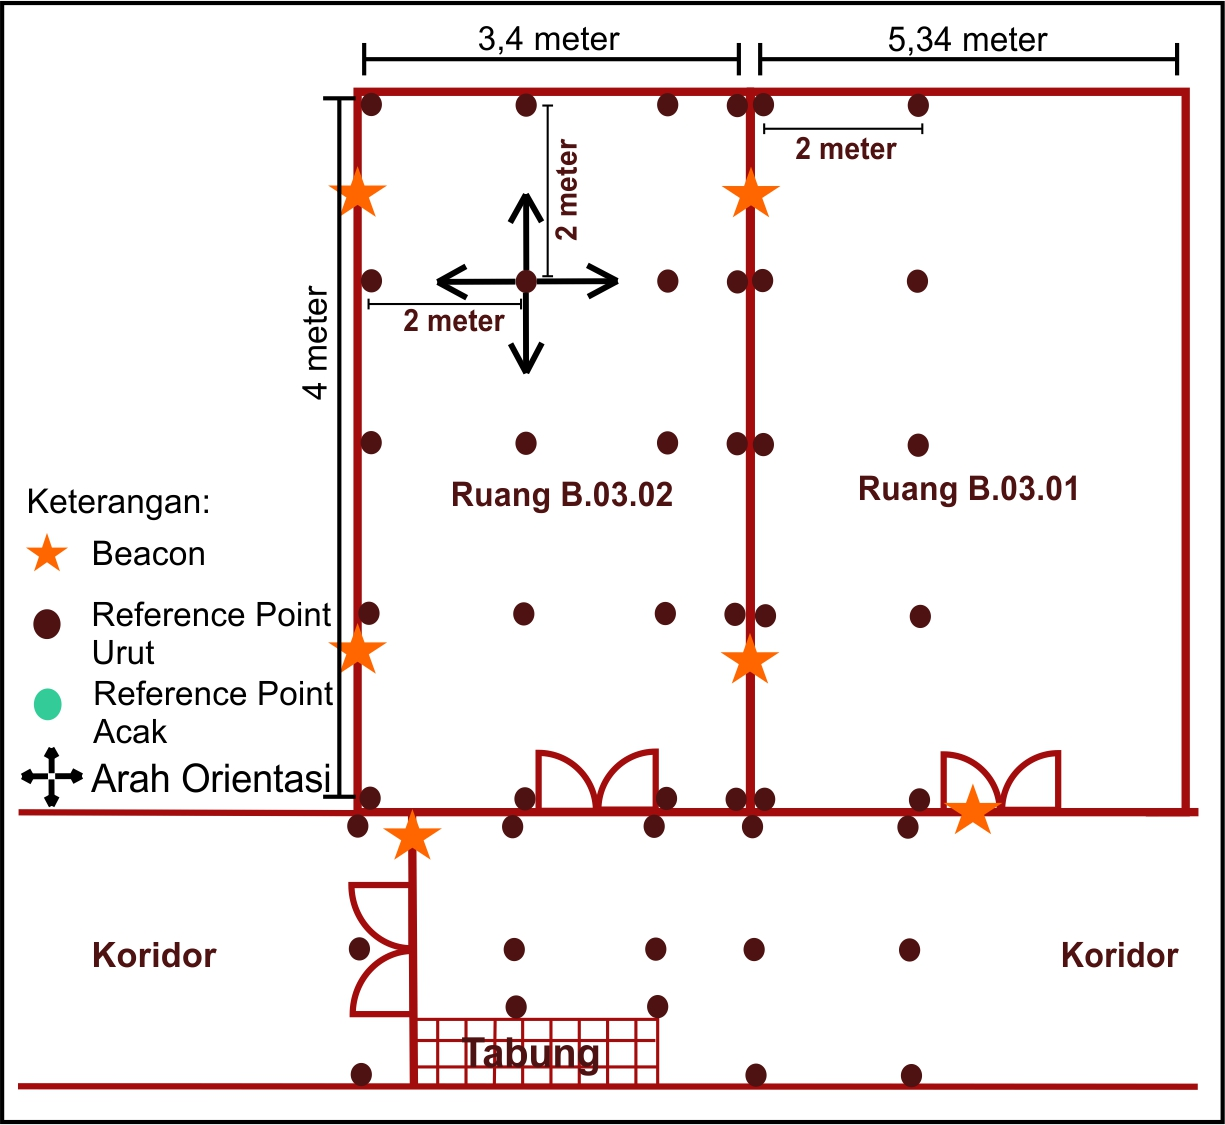
\includegraphics[width=10cm, height=9cm]{gambar/denah/B0302-Urut} }}%
    \qquad
    \subfloat[Reference Point Acak]{{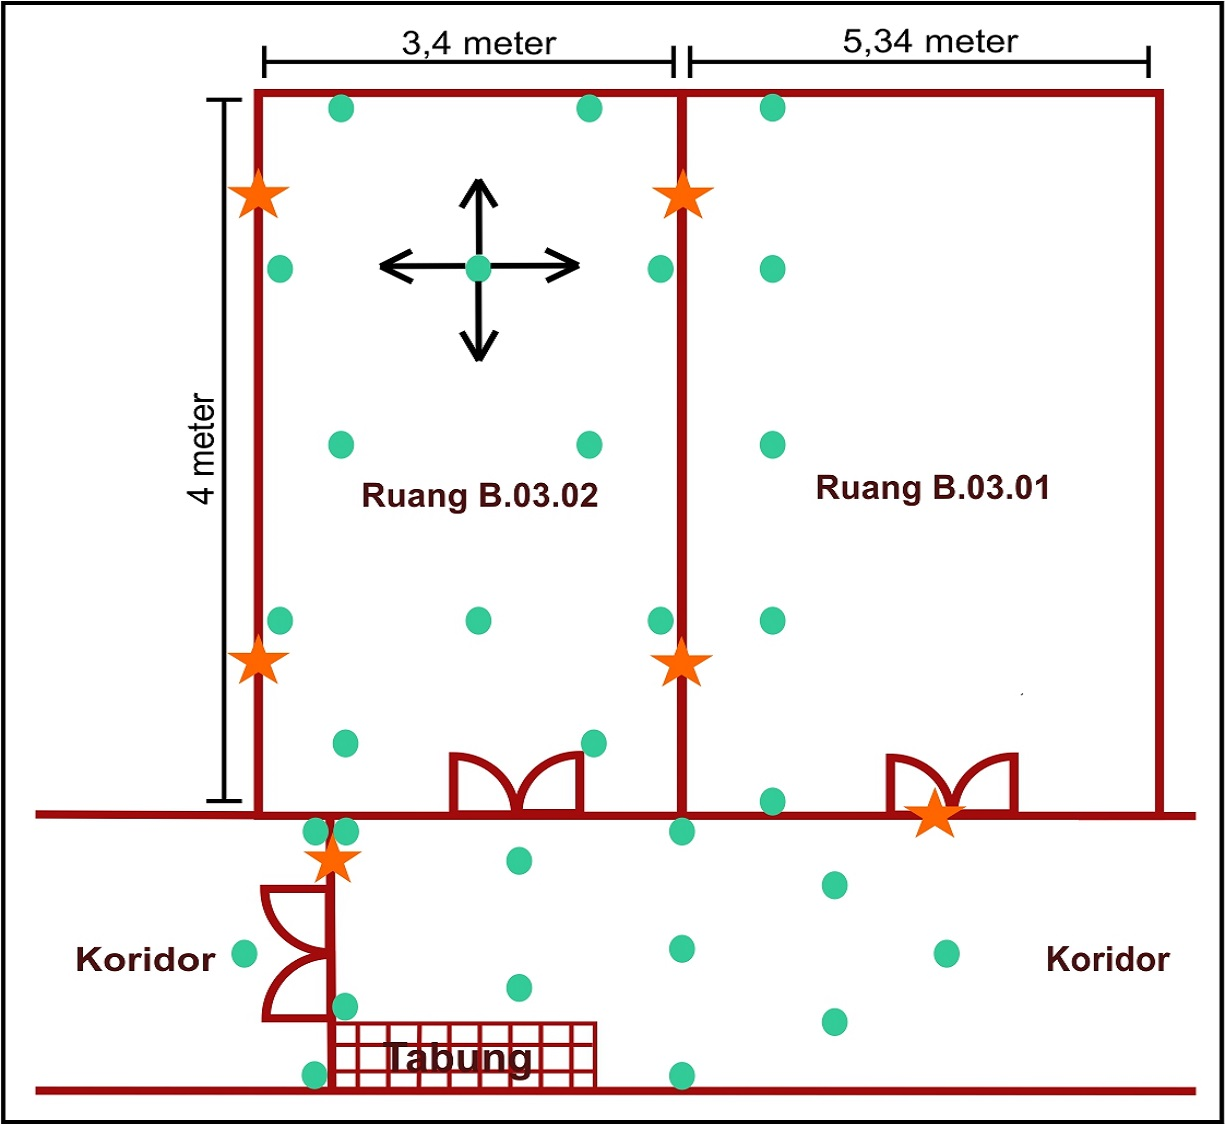
\includegraphics[width=10cm, height=9cm]{gambar/denah/B0302-Acak} }}%
    \caption{Denah Lokasi Penelitian Ruang B.03.02}%
    \label{kelasb0302}%
\end{figure}
\end{landscape}

\begin{figure}[H]
    \centering
    \subfloat[Reference Point Urut]{{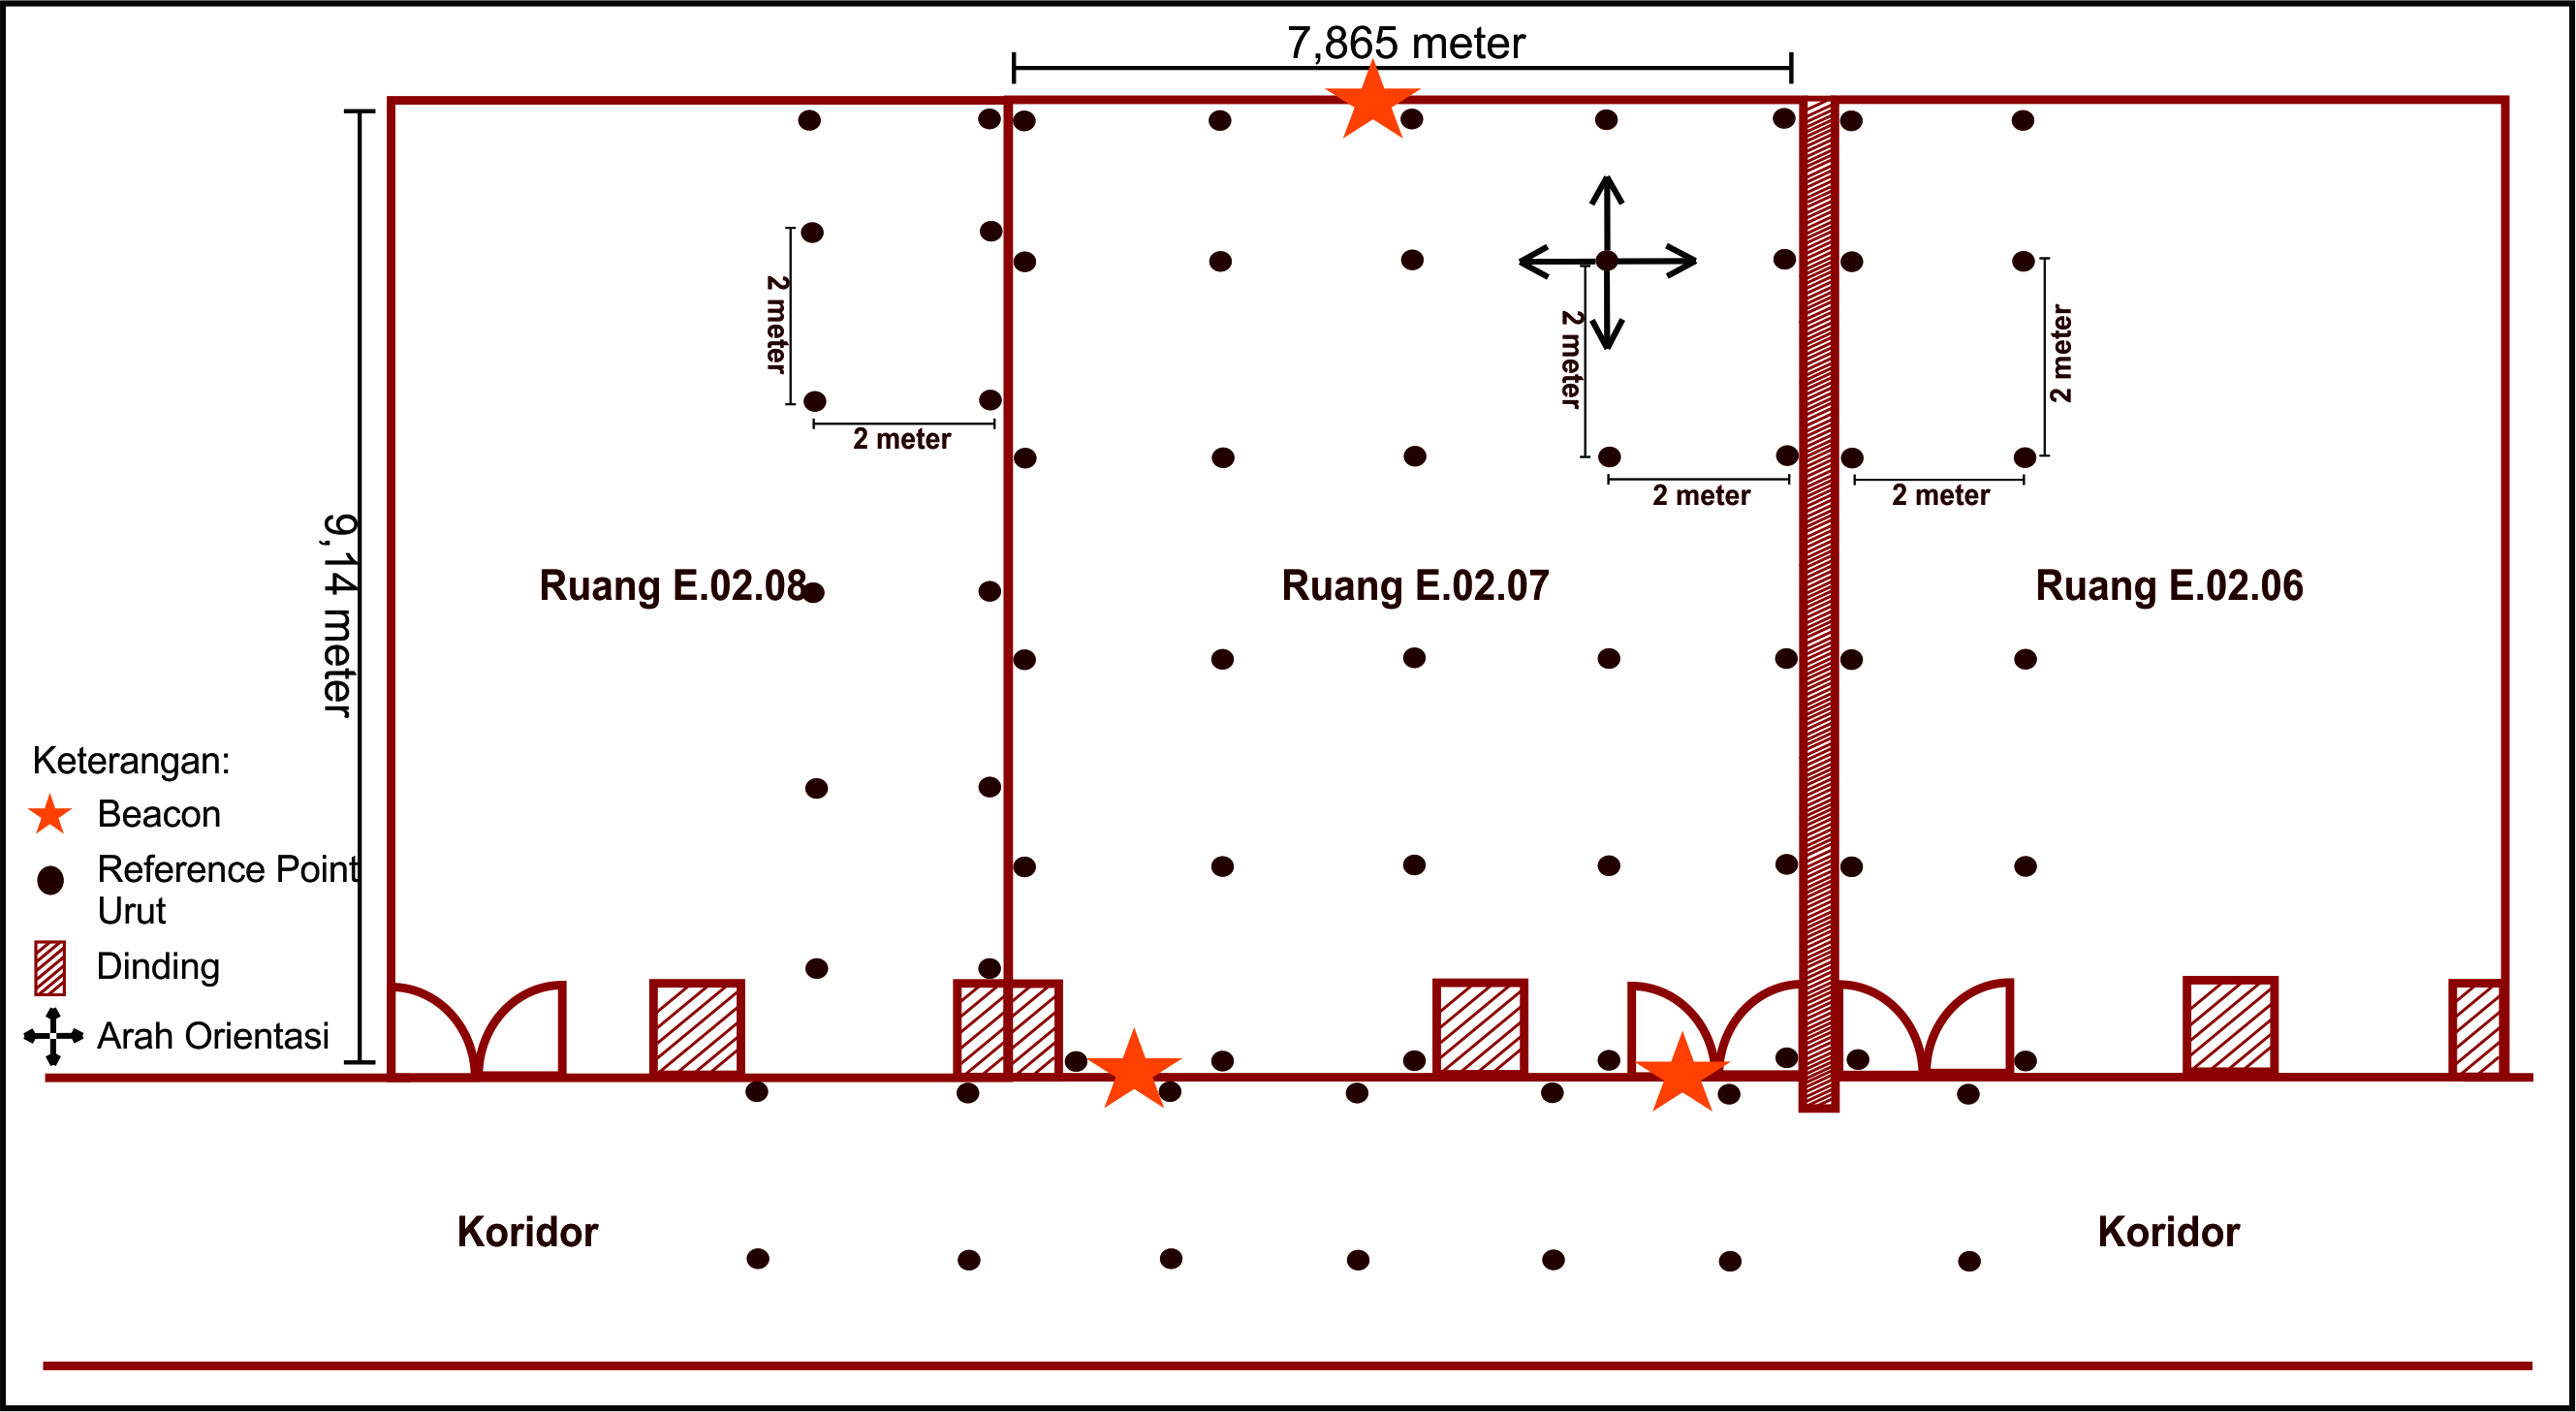
\includegraphics[width=13.3cm, height=8.2cm]{gambar/denah/E0207-Urut} }}%
    \qquad
    \\
    \subfloat[Reference Point Acak]{{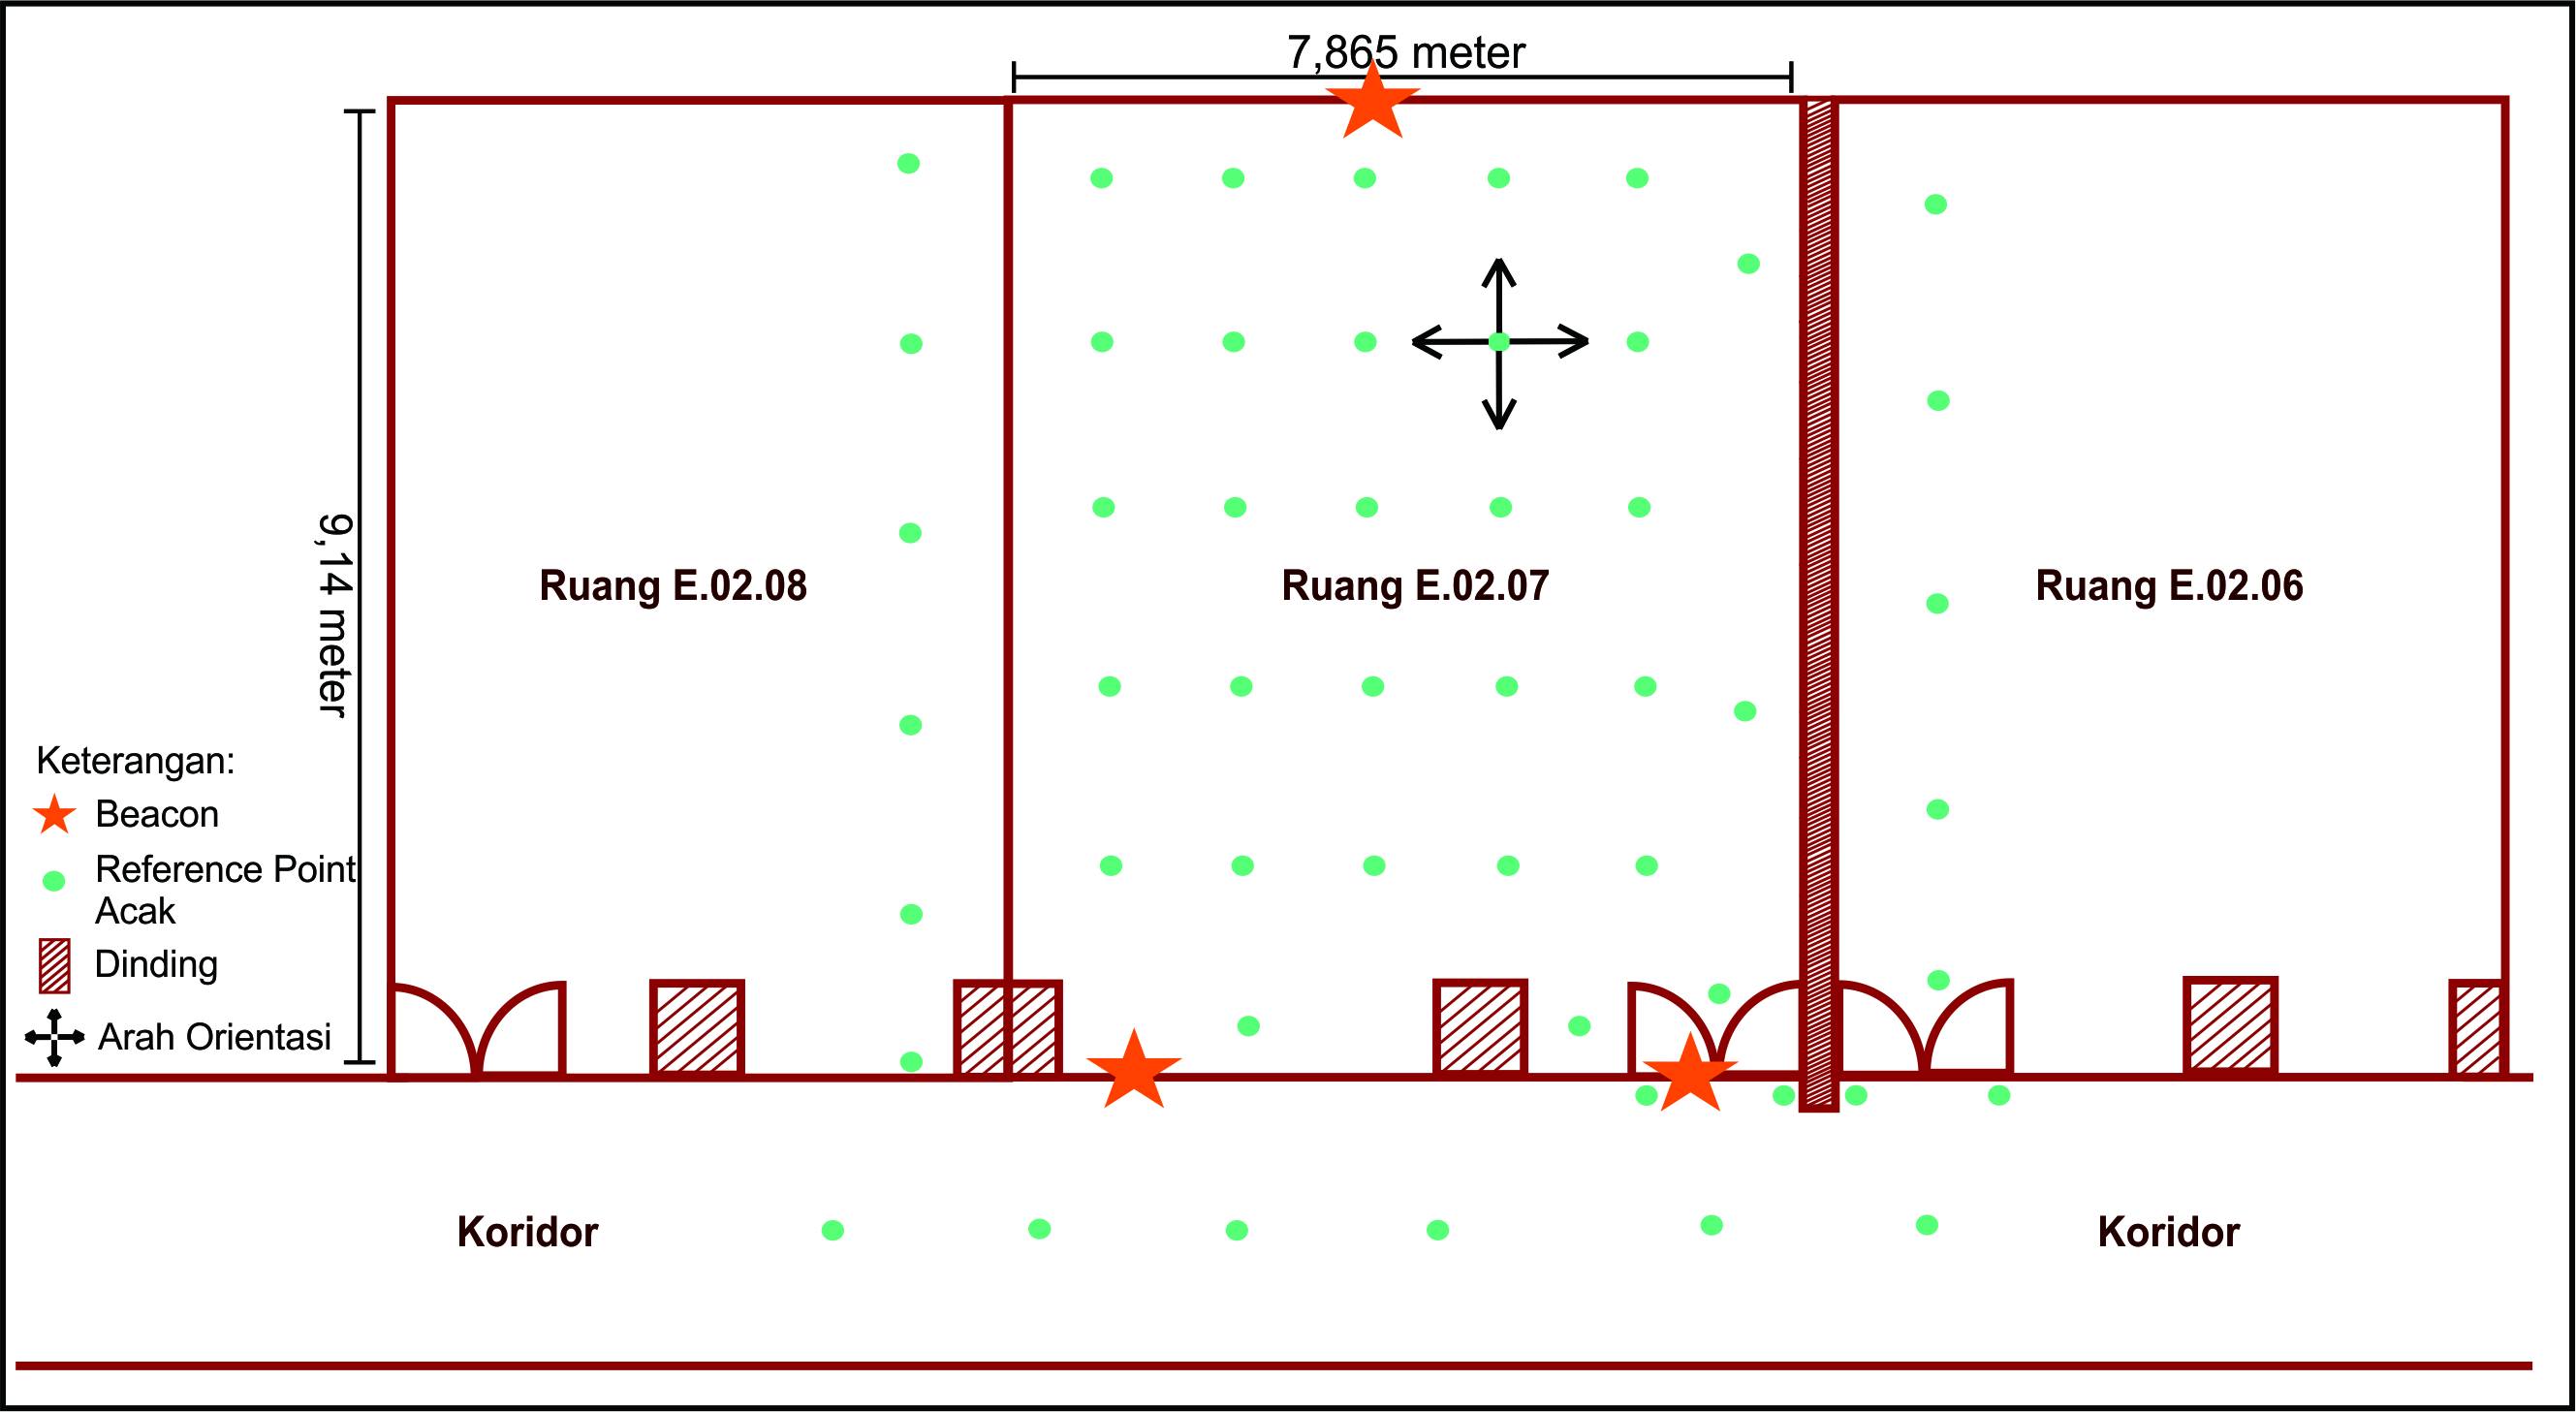
\includegraphics[width=13.3cm, height=8.2cm]{gambar/denah/E0207-Acak} }}%
    \caption{Denah Lokasi Penelitian Ruang E.02.07}%
    \label{kelase0207}%
\end{figure}

\par Proses pemetaan pengambilan kekuatan sinyal berdasarkan letak \textit{reference point} dilakukan dengan menghadap sebanyak 4 arah orientasi, yaitu: depan, kanan, belakang, dan kiri. Penelitian yang dilakukan oleh \cite{Bahl2000} menyebutkan bahwa kekuatan sinyal pada lokasi tertentu cukup bervariasi hingga -5 dBm tergantung pada arah yang dihadap pengguna. Dalam satu arah orientasi, antena \textit{host} yang dimiliki oleh \textit{smartphone} memiliki konektivitas \textit{line-of-sight} (LoS) ke sebuah antena Beacon selama orientasinya berlawanan. Arah orientasi dari tubuh pengguna juga dapat membentuk sebuah halangan dan kekuatan sinyal yang ditangkap juga berbeda. Oleh karena itu, perlu dilakukan pencatatan \textit{direction} (d), dengan menghadap ke depan, ke kanan, ke belakang dan ke kiri tergantung pada pengambilan kekuatan sinyal yang dilakukan \citep{christ1993}. Metode pengambilan kekuatan sinyal setiap Beacon berdasarkan proses survei pemetaan \textit{reference point} disebut dengan metode \textit{Fingerprinting}. Metode \textit{Fingerprinting} dilakukan dengan mengumpulkan dan menyimpan data-data kekuatan sinyal ke dalam basis data aplikasi untuk dijadikan sebagai data \textit{training}.  

%%%%%%%%%%%%%%%%%%%%%%next%%%%%%%%%%%%%%%%%%%%%
\item Pengumpulan Data \textit{Training}
\\
Pengumpulan data \textit {training} bertujuan untuk pembuatan basis data dari data kekuatan sinyal atau nilai RSSI yang didapat dari setiap Beacon. Pengumpulan data \textit{training} (\textit{offline}) dilakukan berdasarkan penentuan letak \textit{reference point} yang telah ditentukan sebelumnya. Pengumpulan data \textit{training} dengan pemetaan metode \textit{Fingerprinting} ini menggunakan Aplikasi Mapping yang telah dibuat dengan fitur-fitur untuk dapat menangkap kekuatan sinyal dari Beacon, kemudian informasi-informasi dari Beacon tersebut seperti MAC Address, nilai RSSI, dan nama ruangan dimana kekuatan sinyal tersebut ditangkap dapat disimpan pada aplikasi ini. Ilustrasi penyimpanan data \textit{training} dengan metode \textit{Fingerprinting} untuk \textit{reference point} urut dapat dilihat pada Tabel \ref{fingerprinting-sequence-point} dan untuk \textit{reference point} acak dapat dilihat pada Table \ref{fingerprinting-random-point}. Orientasi yang tercantum pada kedua gambar tersebut hanya sebagai gambaran bahwa penyimpanan data terhadap suatu posisi diambil berdasarkan 4 arah hadap.

\begin{landscape}
\begin{table}[H]
\caption{Ilustrasi Penyimpanan Data Training Metode \textit{Fingerprinting} pada \textit{Reference Point} Urut.}
\centering
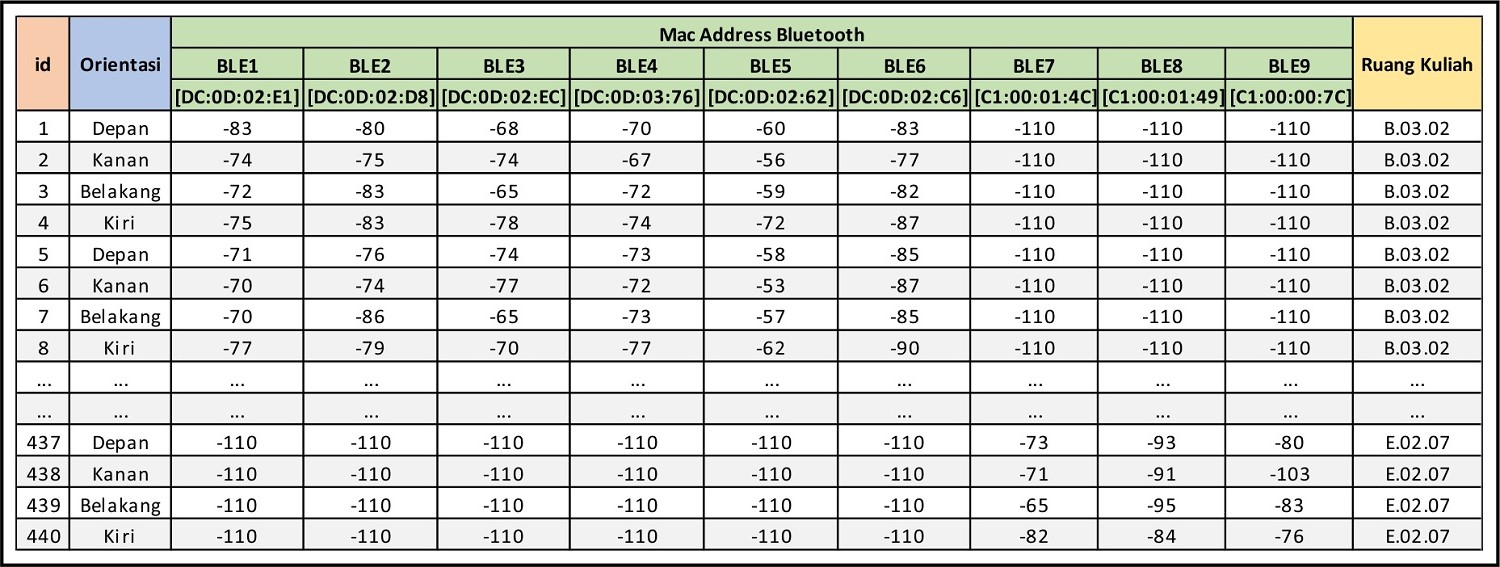
\includegraphics[width=20cm, height=9cm]{gambar/pengumpulan_data/sequence_point.jpg}
\label{fingerprinting-sequence-point}
\end{table}
\end{landscape}

\begin{landscape}
\begin{table}[H]
\caption{Ilustrasi Penyimpanan Data Training Metode \textit{Fingerprinting} pada \textit{Reference Point} Acak.}
\centering
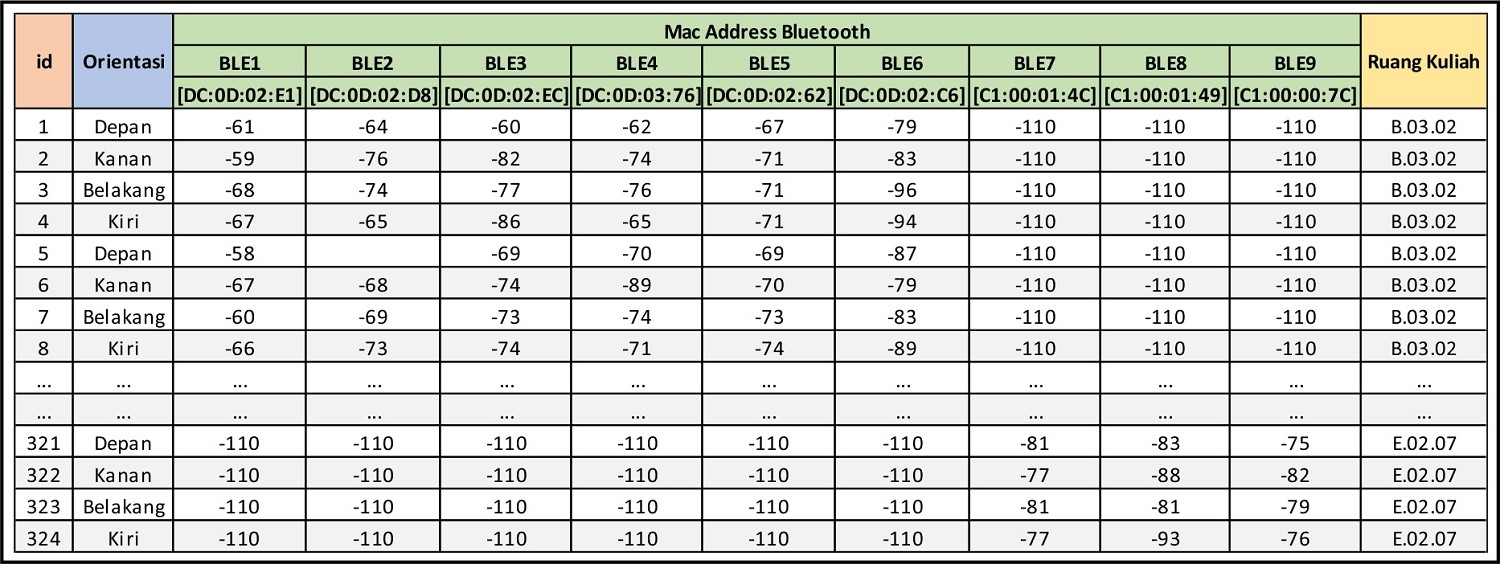
\includegraphics[width=20cm, height=9cm]{gambar/pengumpulan_data/random_point.jpg}
\label{fingerprinting-random-point}
\end{table}
\end{landscape}

\vspace{3cm}

\item Pengumpulan Data Uji
\\
Pengumpulan data uji bertujuan untuk menguji tingkat keberhasilan klasifikasi dengan melihat akurasi tertinggi bergantung pada parameter nilai \textit{k} yang digunakan. Pengumpulan data uji dilakukan setelah pengumpulan data \textit{training} dilakukan. Data uji bertindak seolah-olah kelas label belum diketahui. Data uji tersebut akan dibandingkan dengan data \textit{training} sebagai pengujian nilai \textit{k} terbaik, hasil dari nilai \textit{k} terbaik tersebut akan diimplementasikan pada Aplikasi Kehadiran Dosen dan Aplikasi Kehadiran Mahasiswa untuk memprediksi lokasi pengguna dengan metode klasifikasi K-NN.

\end{enumerate} 
%%%%%%%%%%%%%%%%%%%%%%%%%%%%%%%%%%%%%%%%%%%%%%%%%%%%%%%%%%%%%%%%%%%%%%%%%%%%%%%%%%%%%%%%%%%%%%%%%%%%%%%%%%%%%%%%%%%%%%%%%%%
%TESTING KNN%
\subsection{Pengujian Akurasi dengan Metode Klasifikasi K-NN}

\par Pengujian ini dilakukan dengan tujuan untuk mengetahui tingkat keberhasilan dari proses klasifikasi lokasi pengguna berdasarkan \textit{reference point} yang digunakan. Pengujian ini dilakukan dengan menggunakan parameter variasi nilai \textit{k} yang digunakan dalam penelitian ini, yaitu 3, 5 dan 7. Variasi nilai \textit{k} pada metode klasifikasi K-NN, digunakan untuk mencari nilai \textit{k} yang optimal sehingga tingkat akurasi tertinggi didapatkan. 

\par Proses klasifikasi yang diterapkan pada penelitian ini adalah analisa kuantitatif dengan membandingkan hasil perhitungan  nilai \textit{F-Measure} dari setiap parameter nilai \textit{k} yang ada. Parameter nilai \textit{k} terbaik ditentukan dari nilai \textit{F-Measure} terbesar dengan membandingkan parameter-parameter klasifikasi yang telah ditetapkan sebelumnya. Perhitungan nilai \textit{F-Measure} dilakukan berdasarkan hasil klasifikasi yang dapat dilihat pada Tabel \ref{tabel-matrix}.

\begin{table}[H]
\centering
\caption{Matriks Konfusi \citep{han2006}.}
\label{tabel-matrix}
\begin{tabular}{ccccl}
\cline{2-4}
\multicolumn{1}{c|}{}                                                                                      & \multicolumn{3}{c|}{\textbf{Diprediksi Sebagai}}                                                                      &  \\ \cline{1-4}
\multicolumn{1}{|c|}{\multirow{3}{*}{\textbf{\begin{tabular}[c]{@{}c@{}}Kelas\\ Sebenarnya\end{tabular}}}} & \multicolumn{1}{c|}{}                 & \multicolumn{1}{c|}{\textbf{Positif}} & \multicolumn{1}{c|}{\textbf{Negatif}} &  \\ \cline{2-4}
\multicolumn{1}{|c|}{}                                                                                     & \multicolumn{1}{c|}{\textbf{Positif}} & \multicolumn{1}{c|}{TP}               & \multicolumn{1}{c|}{FN}               &  \\ \cline{2-4}
\multicolumn{1}{|c|}{}                                                                                     & \multicolumn{1}{c|}{\textbf{Negatif}} & \multicolumn{1}{c|}{FP}               & \multicolumn{1}{c|}{TN}               &  \\ \cline{1-4}
\multicolumn{1}{l}{}                                                                                       & \multicolumn{1}{l}{}                  & \multicolumn{1}{l}{}                  & \multicolumn{1}{l}{}                  & 
\end{tabular}
\end{table}
Keterangan:\newline
$TP$ = \textit{True} Positif. \newline
$FP$ = \textit{False} Positif. \newline
$FN$ = \textit{False} Negatif. \newline
$TN$ = \textit{True} Negatif. \newline
\par Tabel \ref{tabel-matrix} merepresentasikan prediksi dan kelas sebenarnya, sehingga dapat digunakan untuk menentukan \textit{precision}, \textit{recall}, dan \textit{F-Measure}. \textit{Precision} ($p$) merupakan perbandingan antara data yang benar diklasifikasikan positif dengan total data yang diklasifikasikan positif yang dapat dilihat dengan rumus: 

\begin{equation}
p= \frac{TP} {TP+FP}
\end{equation}
%end precision

\par Recall ($r$) merupakan perbandingan antara data yang benar diklasifikasikan positif dengan total data yang seharusnya positif yang dapat dilihat dengan rumus:

\begin{equation}
r= \frac{TP} {TP+FN} 
\end{equation}
\newline
\par Rumus untuk menghitung \textit{F-Measure} $(F)$ adalah sebagai berikut:

\begin{equation}
F=2 \cdot \frac{p.r} {p+r}
\end{equation}
\newline
Keterangan:\newline
$p$ = \textit{precision}. \newline
$r$ = \textit{recall}. 

\subsection{Pembuatan Aplikasi Kehadiran dan Aplikasi Web Admin}
\begin{enumerate}

\item Aplikasi Kehadiran Dosen
\newline
Aplikasi ini merupakan aplikasi \textit{mobile} berbasis Android yang berguna untuk mempermudah dosen melakukan proses pencatatan kehadiran perkuliahan di Jurusan Informatika Unsyiah, yang dikembangkan dengan konsep \textit{Indoor Positioning System}. Aplikasi ini bekerja apabila perangkat \textit{smartphone} sudah mendukung Bluetooth 4.0, dikarenakan aplikasi ini menangkap kekuatan sinyal atau nilai RSSI dari Beacon yang terintegrasi BLE di dalamnya. Kekuatan sinyal yang ditangkap akan dilakukan perhitungan menggunakan metode klasifikasi K-NN, \textit{output} dari perhitungan tersebut adalah prediksi lokasi dosen yang akan dikirim ke \textit{web services} secara \textit{background process} sebagai bukti kehadiran. Adapun fitur-fitur yang tersedia adalah sebagai berikut:

\begin {itemize}
\itemsep0em
\item Memproses Pencatatan Data Kehadiran \newline
Pada aplikasi ini, dosen diwajibkan untuk memulai proses pencatatan data kehadiran perkuliahan dengan menekan tombol \textbf{start attendance}. Proses pencatatan data kehadiran perkuliahan dapat dimulai apabila sudah pada waktunya dan tidak dapat dimulai apabila dosen sudah terlambat selama 50 menit. Aplikasi akan memproses kehadiran dosen sampai mata kuliah berakhir.

\item Menampilkan Jadwal Perkuliahan \newline
Aplikasi dapat menampilkan jadwal perkuliahan yang dimiliki oleh masing-masing dosen per-harinya. Apabila dosen menekan salah satu jadwal perkuliahan, akan diarahkan ke halaman informasi mata kuliah tersebut seperti: kode mata kuliah, nama mata kuliah, waktu perkuliahan, nama ruangan, dan jumlah mahasiswa yang mengambil mata kuliah.

\item Melihat Daftar Mahasiswa \newline
Aplikasi ini menyediakan fitur agar dosen dapat melihat daftar nama mahasiswa yang mengambil suatu mata kuliah. 

\end{itemize}

\item Aplikasi Kehadiran Mahasiswa
\newline
Aplikasi ini merupakan aplikasi \textit{mobile} berbasis Android yang berguna untuk mempermudah mahasiswa melakukan proses pencatatan kehadiran perkuliahan di Jurusan Informatika Unsyiah, yang dikembangkan dengan konsep \textit{Indoor Positioning System}. Aplikasi ini bekerja apabila perangkat \textit{smartphone} sudah mendukung Bluetooth 4.0, dikarenakan aplikasi ini menangkap kekuatan sinyal atau nilai RSSI dari Beacon yang terintegrasi BLE di dalamnya. Kekuatan sinyal yang ditangkap akan dilakukan perhitungan menggunakan metode klasifikasi K-NN, \textit{output} dari perhitungan tersebut adalah prediksi lokasi mahasiswa yang akan dikirim ke \textit{web services} secara \textit{background process} sebagai bukti kehadiran. Adapun fitur-fitur yang tersedia adalah sebagai berikut:
 
\begin {itemize}
\itemsep0em
\item Memproses Pencatatan Data Kehadiran \newline
Mahasiswa dapat memulai proses pencatatan data kehadiran apabila dosen sudah memulai perkuliahan. Aplikasi akan memproses pencatatan data kehadiran mahasiswa sampai mata kuliah berakhir.

\item Menampilkan Jadwal Perkuliahan \newline
Aplikasi memiliki fitur untuk menampilkan jadwal perkuliahan yang dimiliki oleh masing-masing mahasiswa per-harinya. Jadwal perkuliahan yang ditampilkan berisi informasi seperti: nama dosen yang mengajar, kode mata kuliah, nama mata kuliah, ruangan, dan waktu perkuliahan.

\item Melihat Mata Kuliah \newline
Pada aplikasi ini, mahasiswa dapat melihat daftar mata kuliah yang diambil pada sistem KRS Online. Aplikasi menampilkan informasi-informasi setiap mata kuliah tersebut.
\end{itemize}

\item Aplikasi Rekap Kehadiran Mahasiswa dan Kehadiran Dosen
\newline
Aplikasi ini merupakan aplikasi berbasis web yang berguna untuk mempermudah staf dan admin untuk merekap data kehadiran dosen dan mahasiswa di Jurusan Informatika Unsyiah. Aplikasi ini menyajikan data daftar kehadiran dosen dan mahasiswa berdasarkan pada kode mata kuliah dan tanggal pelaksanaan perkuliahan yang dipilih. Aplikasi ini dapat mengunduh data rekapitulasi daftar kehadiran dosen dan mahasiswa ke dalam bentuk format CSV. 

\end{enumerate}
%%%%%%%%%%%%%%%%%%%%%%%%%%%%%%%%%%%%%%%%%%%%%%%%%%%%%%%%%%%%%%%%%%%%%%%%%%%%%%%%%%%%%%%%%%%%%%%%%%%%%%%%%%%%%%%%%%%%%%%%%%%%%%%
\subsection{Pengujian Fungsionalitas dengan Metode Black Box}
\par Pengujian \textit{Black Box} berfokus pada spesifikasi fungsionalitas dari sistem yang telah dibuat dengan mengeksekusi dan menjalankan sistem tersebut apakah sesuai dengan alur bisnis yang diinginkan. Pengujian ini melihat fungsi yang tidak sesuai pada sistem, kesalahan-kesalahan sistem dalam mengerjakan suatu perintah, dan kesalahan-kesalahan pada struktur data dan akses basis data. 

\subsection{Pengujian Usabilitas dengan Metode SUS}
\par Salah satu prinsip utama yang dijadikan sebagian tolak ukur keberhasilan dari pengembangan perangkat lunak adalah nilai pengujian itu sendiri. \textit{Usability Testing} dilakukan untuk melihat dan mengevaluasi sebuah produk atau jasa dengan cara menguji kepada calon pengguna dengan menggunakan metode SUS. SUS terdiri dari 10 pertanyaan dengan menggunakan skala likert 1-5. Berikut daftar pertanyaan-pertanyaan metode SUS dapat dilihat pada Tabel \ref{tabel-pertanyaan-sus}.  
%TABEL PERTANYAAN SUS%
\begin{table}[H]
\center
\caption{Daftar Pertanyaan Metode SUS \citep{Sharfina2016}}
\label{tabel-pertanyaan-sus}
\begin{tabular}{|c|l|l}
\cline{1-2}
\textbf{\begin{tabular}[c]{@{}c@{}}Kode \\ Pertanyaan\end{tabular}} & \multicolumn{1}{c|}{\textbf{Daftar Pertanyaan}}                                                                               &  \\ \cline{1-2}
$R1$                                                                  & Saya berpikir akan menggunakan sistem ini                                                                                     &  \\ \cline{1-2}
$R2$                                                                  & Saya merasa sistem ini sulit untuk digunakan                                                                                  &  \\ \cline{1-2}
$R3$                                                                  & Saya merasa sistem ini mudah digunakan                                                                                        &  \\ \cline{1-2}
$R4$                                                                  & \begin{tabular}[c]{@{}l@{}}Saya akan membutuhkan bantuan orang lain \\ untuk menggunakan sistem ini\end{tabular}              &  \\ \cline{1-2}
$R5$                                                                  & \begin{tabular}[c]{@{}l@{}}Saya merasa fitur-fitur pada sistem ini sudah \\ berjalan dengan sebagaimana mestinya\end{tabular} &  \\ \cline{1-2}
$R6$                                                                  & \begin{tabular}[c]{@{}l@{}}Saya merasa banyak hal-hal yang tidak \\ konsisten (tidak serasi) pada sistem ini\end{tabular}     &  \\ \cline{1-2}
$R7$                                                                  & \begin{tabular}[c]{@{}l@{}}Saya merasa orang lain dapat memahami cara\\ menggunakan aplikasi ini dengan cepat\end{tabular}    &  \\ \cline{1-2}
$R8$                                                                  & Saya merasa aplikasi ini membingungkan                                                                                        &  \\ \cline{1-2}
$R9$                                                                  & \begin{tabular}[c]{@{}l@{}}Saya merasa nyaman (tidak ada hambatan) \\ dalam menggunakan sistem ini\end{tabular}               &  \\ \cline{1-2}
$R10$                                                                 & \begin{tabular}[c]{@{}l@{}}Saya perlu membiasakan diri terlebih dahulu \\ sebelum menggunakan aplikasi ini\end{tabular}       &  \\ \cline{1-2}
\end{tabular}
\end{table}

\par Rumus untuk menghitung skor akhir metode SUS \citep{Brooke1996}, dapat dilihat dari persamaan berikut.
\begin{equation}
skorSUS = (\sum_{9}^{i} (Ri - 1) + \sum_{10}^{j} (5 - Rj)) * 2,5
\end{equation}
\newline
Keterangan:\newline
$R$ = daftar pertanyaan pada metode SUS. \newline
$i$ = angka ganjil 1, 3, 5, 7, dan 9. \newline
$j$ = angka genap 2, 4, 6, 8, dan 10.
\newline 

\par Tingkat nilai skala pengujian menentukan apakah sistem tersebut layak digunakan, bermanfaat, diterima oleh \textit{user} dan bertahan lama penggunaannya. Sebuah sistem dengan nilai pengujian yang tinggi membuat sistem tersebut menjadi populer dalam waktu yang lama dan penggunaannya yang luas, karena banyak individu akan merasakan manfaat dari kehadiran sistem tersebut. Sedangkan sistem dengan nilai pengujian yang rendah, seringkali diabaikan oleh pengguna walaupun dibuat berdasarkan kebutuhan dan menghasilkan sumber daya yang banyak. Berdasarkan dari skor akhir SUS tersebut, dapat diketahui bahwa seberapa tinggi tingkat \textit{usability} rancangan sistem yang dikembangkan. Tabel \ref{tabelsus} menunjukkan nilai interpretasi yang digunakan.

\begin{table}[H]
\center
\caption{Interpretasi skor SUS \citep{Bangoor2009}.}
\label{tabelsus}
\begin{tabular}{|c|c|lll}
\cline{1-2}
\textbf{Skor SUS} & \textbf{Interprestasi} &  &  &  \\ \cline{1-2}
\textless{}50     & Tidak Dapat Diterima   &  &  &  \\ \cline{1-2}
50-70             & Marginal               &  &  &  \\ \cline{1-2}
\textgreater{}70  & Dapat Diterima         &  &  &  \\ \cline{1-2}
\end{tabular}
\end{table}

%%%%%%%%%%%%%%%%%%%%%%%%%%%%%%%%%%%%%%%%%%%%%%%%%%%%%%%%%%%%%%%%%%%%%%%%%%%%%%%%%%%%%%%%%%%%%%%%%%%%%%%%%%%%%%%%
\subsection{Analisis Keakuratan}
Penelitian ini memiliki dua analisis keakuratan dalam penentuan lokasi pengguna. Analisis keakuratannya adalah sebagai berikut:
\begin{enumerate}[1.]
\item Membandingkan tingkat keakuratan klasifikasi antara \textit{reference point} urut dan \textit{reference point} acak.
\item Membandingkan tingkat keakuratan dalam memprediksi lokasi pengguna menggunakan jumlah Beacon yang berbeda, yaitu dengan jumlah 3 Beacon dan 6 Beacon.
\end{enumerate}


	%-------------------------------------------------------------------------------
%                            BAB IV
%               		HASIL DAN PEMBAHASAN
%-------------------------------------------------------------------------------
\fancyhf{} 
\fancyfoot[C]{\thepage}
\chapter{HASIL DAN PEMBAHASAN}
	\section{\uppercase{ANALISIS KEBUTUHAN}}
	
	Hasil dari analisis kebutuhan yang telah dilakukan adalah mendapatkan kelompok pengguna yang akan terlibat dalam penelitian dan \textit{use case diagram} untuk masing-masing pengguna. Berikut hasil analisis kebutuhan dari sistem yang dibangun.
	
	\subsection{Kelompok Pengguna}
	Kelompok pengguna dari aplikasi ini telah dapat diidentifikasikan pada tahap analisis kebutuhan pada sistem. terdapat 2 kelompok pengguna yang menggunakan aplikasi ini:
		 \begin{enumerate}[1.]
		 	\item Peneliti
		 		\newline Pengguna yang menggunakan Aplikasi Mapping berbasis Android untuk melakukan pemetaan kekuatan sinyal atau nilai RSSI dari Beacon. 
		 	\item Dosen
		 		\newline Pengguna yang menggunakan Aplikasi Kehadiran Dosen berbasis Android untuk melakukan pencatatan kehadiran sebagai pengajar suatu mata kuliah.
		 	\item Mahasiswa
		 		\newline Pengguna yang menggunakan Aplikasi Kehadiran berbasis Android untuk melakukan pencatatan kehadiran sebagai peserta belajar suatu mata kuliah.
		 	\item Admin
		 		\newline Pengguna yang menggunakan Aplikasi Rekap Kehadiran Dosen dan Mahasiswa berbasis web untuk memantau dan merekap kehadiran dosen dan mahasiswa pada suatu mata kuliah.
		 	\end{enumerate}
	
	\subsection{Use Case Diagram}
	\textit{Use case} merupakan pemodelan untuk mendeskripsikan sebuah interaksi antara satu atau lebih aktor dengan sistem yang dibuat. Secara kasar, \textit{use case} digunakan untuk mengetahui fungsi apa saja yang ada di dalam sebuah sistem dan siapa saja yang berhak menggunakan fungsi-fungsi itu \citep{Rosa2015}. \textit{Use Case Diagram} dari sistem yang telah dibangun dapat dilihat pada Gambar \ref{usecasemapping}, Gambar \ref{usecasedosen}, Gambar \ref{usecasemahasiswa} dan Gambar \ref{usecaseadmin}.
	
	\begin{figure}[H]
		\center
		\shadowbox
		{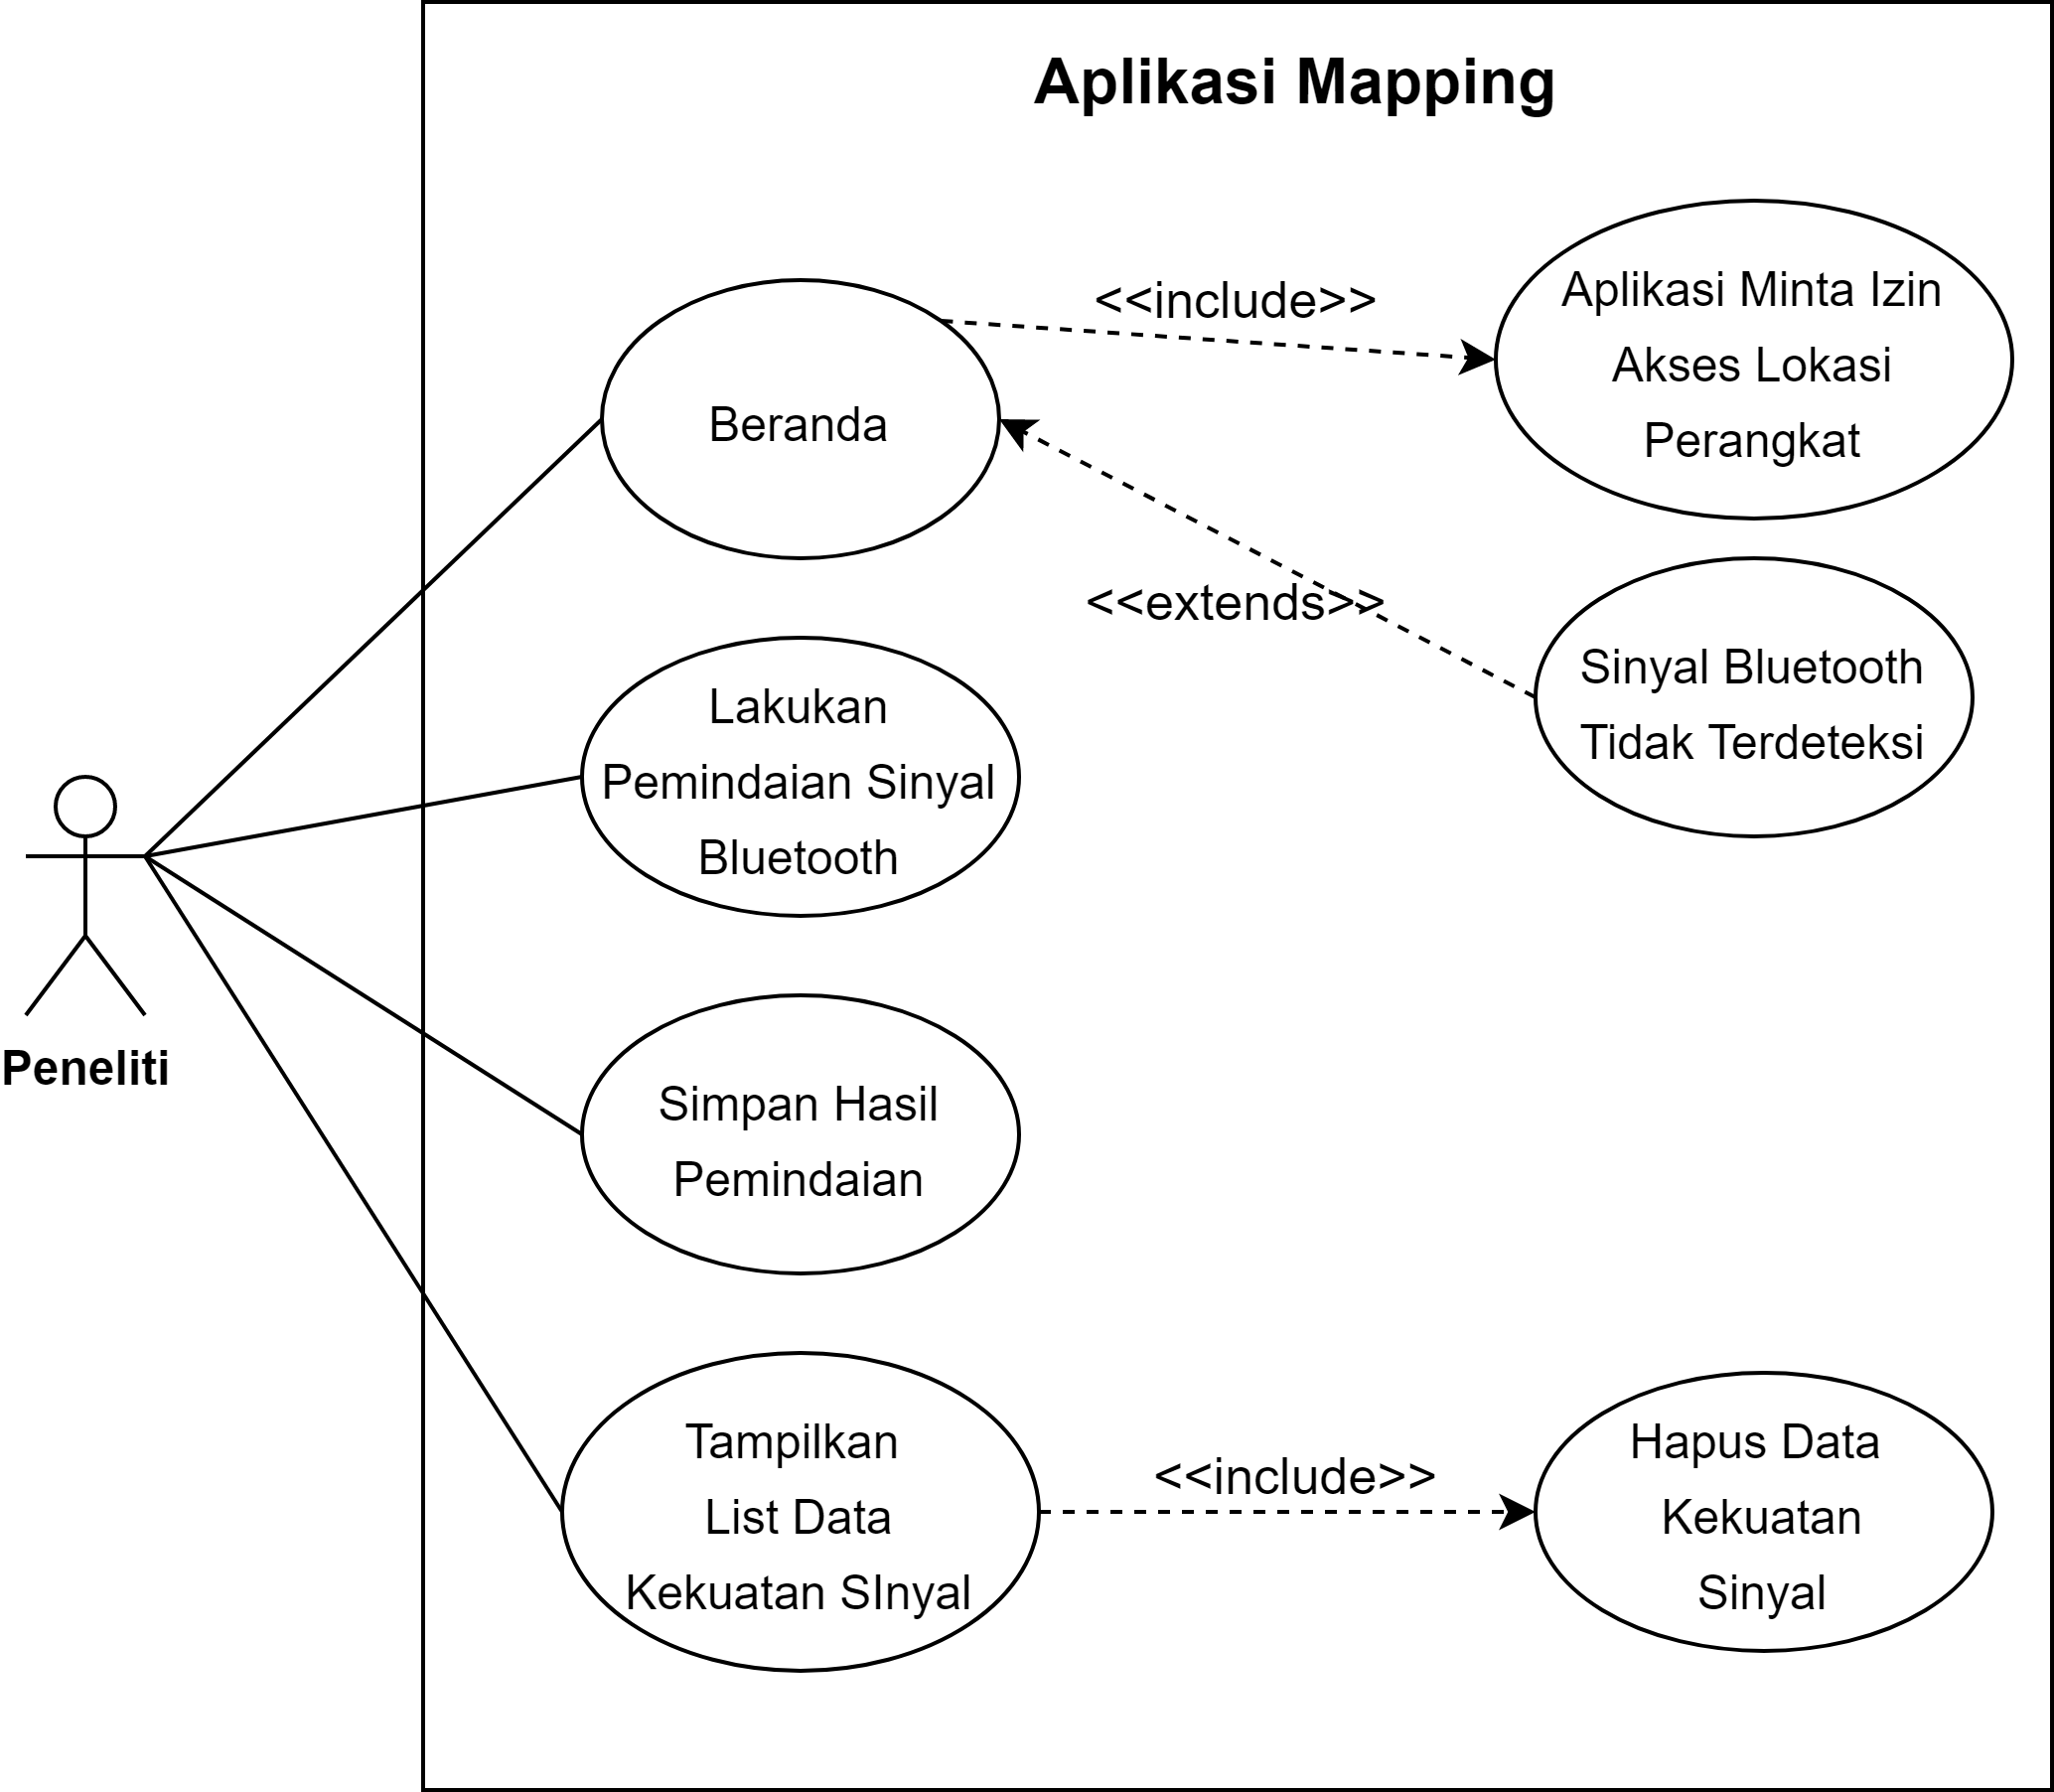
\includegraphics [width=7.5cm, height=7cm]{gambar/model/use-case-mapping}}
		\caption{\textit{Use Case Diagram} Aplikasi Mapping.}
		\label{usecasemapping}
	\end{figure}
	
\par Gambar \ref{usecasemapping} diatas menjelaskan aktivitas yang dapat dilakukan oleh peneliti saat menggunakan aplikasi. Ketika peneliti membuka aplikasi, muncul halaman beranda. Selanjutnya, peneliti diminta untuk mengizinkan aplikasi mengakses lokasi pada perangkat. Kemudian, peneliti dapat melakukan pemindaian kekuatan sinyal setelah menghidupkan Bluetooth pada perangkat. Setelah itu, hasil dari pemindaian kekuatan sinyal tersebut disimpan, lalu dapat ditampilkan pada sebuah halaman. Pengguna juga dapat menghapus data-data kekuatan sinyal sesuai keinginan.
\fancyhf{} 
\fancyfoot[R]{\thepage}

\begin{figure}[H] 
		\center
		\shadowbox
		{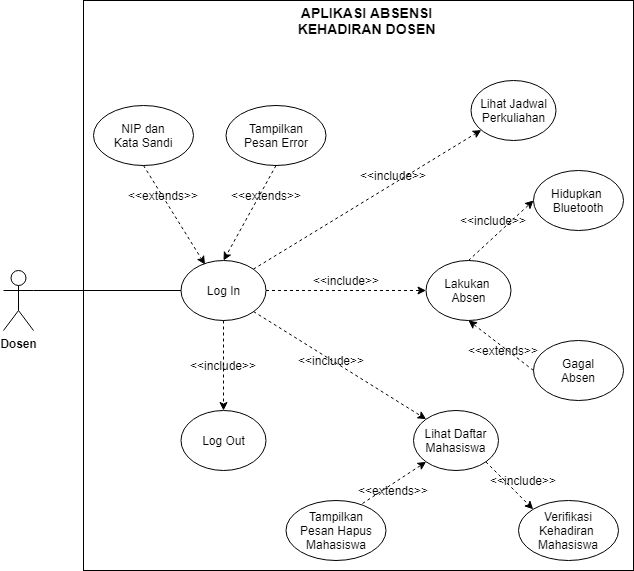
\includegraphics [width=10cm, height=9cm]{gambar/model/use-case-dosen}}
		\caption{\textit{Use Case Diagram} Aplikasi Kehadiran Dosen.}
		\label{usecasedosen}
	\end{figure}

\par Gambar \ref{usecasedosen} menjelaskan aktivitas yang dapat dilakukan oleh dosen saat menggunakan aplikasi. Aktivitas pertama yang dilakukan adalah melakukan \textit{log in} ke aplikasi dengan memasukkan Nomor Induk Pegawai (NIP) dan kata sandi. Setelah melakukan \textit{log in}, dosen dapat menikmati fitur-fitur yang tersedia seperti melihat jadwal perkuliahan, memulai proses kehadiran dengan syarat keadaan Bluetooth pada perangkat dalam keadaan hidup dan melihat daftar mahasiswa yang mengambil suatu mata kuliah. Aktivitas yang terakhir adalah \textit{log out}, yaitu aktivitas yang berfungsi untuk keluar dari aplikasi. Apabila dosen telah melakukan \textit{log out}, maka dosen harus melakukan \textit{log in} kembali ke aplikasi.
	
	\begin{figure}[H] 
		\center
		\shadowbox
		{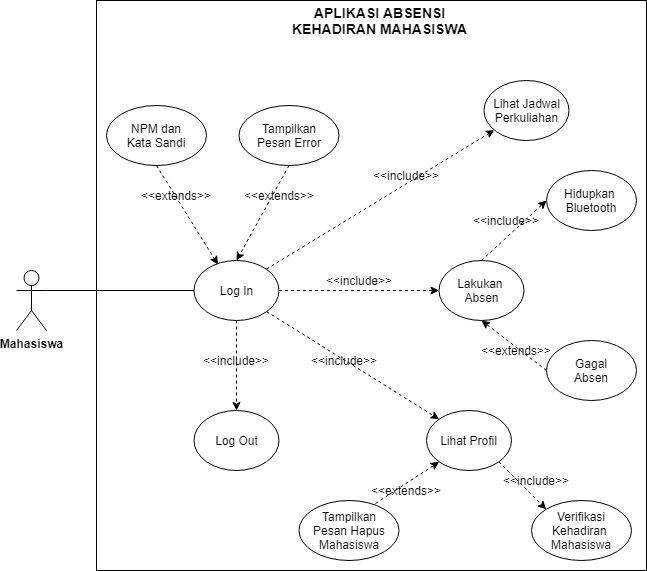
\includegraphics [width=10cm, height=9.5cm]{gambar/model/use-case-mahasiswa}}
		\caption{\textit{Use Case Diagram} Aplikasi Kehadiran Mahasiswa.}
		\label{usecasemahasiswa}
	\end{figure}
	
\par Gambar \ref{usecasemahasiswa} diatas menjelaskan aktivitas yang dapat dilakukan oleh mahasiswa saat menggunakan aplikasi. Aktivitas pertama yang dilakukan adalah melakukan \textit{log in} ke aplikasi dengan memasukkan Nomor Pokok Mahasiswa (NPM) dan kata sandi. Setelah melakukan \textit{log in}, mahasiswa dapat menikmati fitur-fitur yang tersedia seperti melihat jadwal perkuliahan, memulai proses kehadiran dengan syarat keadaan Bluetooth pada perangkat dalam keadaan hidup dan melihat profil data diri. Aktivitas yang terakhir adalah \textit{log out}, yaitu aktivitas yang berfungsi untuk keluar dari aplikasi. Apabila mahasiswa telah melakukan \textit{log out}, maka mahasiswa harus melakukan \textit{log in} kembali ke aplikasi.

	\begin{figure}[H] 
		\center
		\shadowbox
		{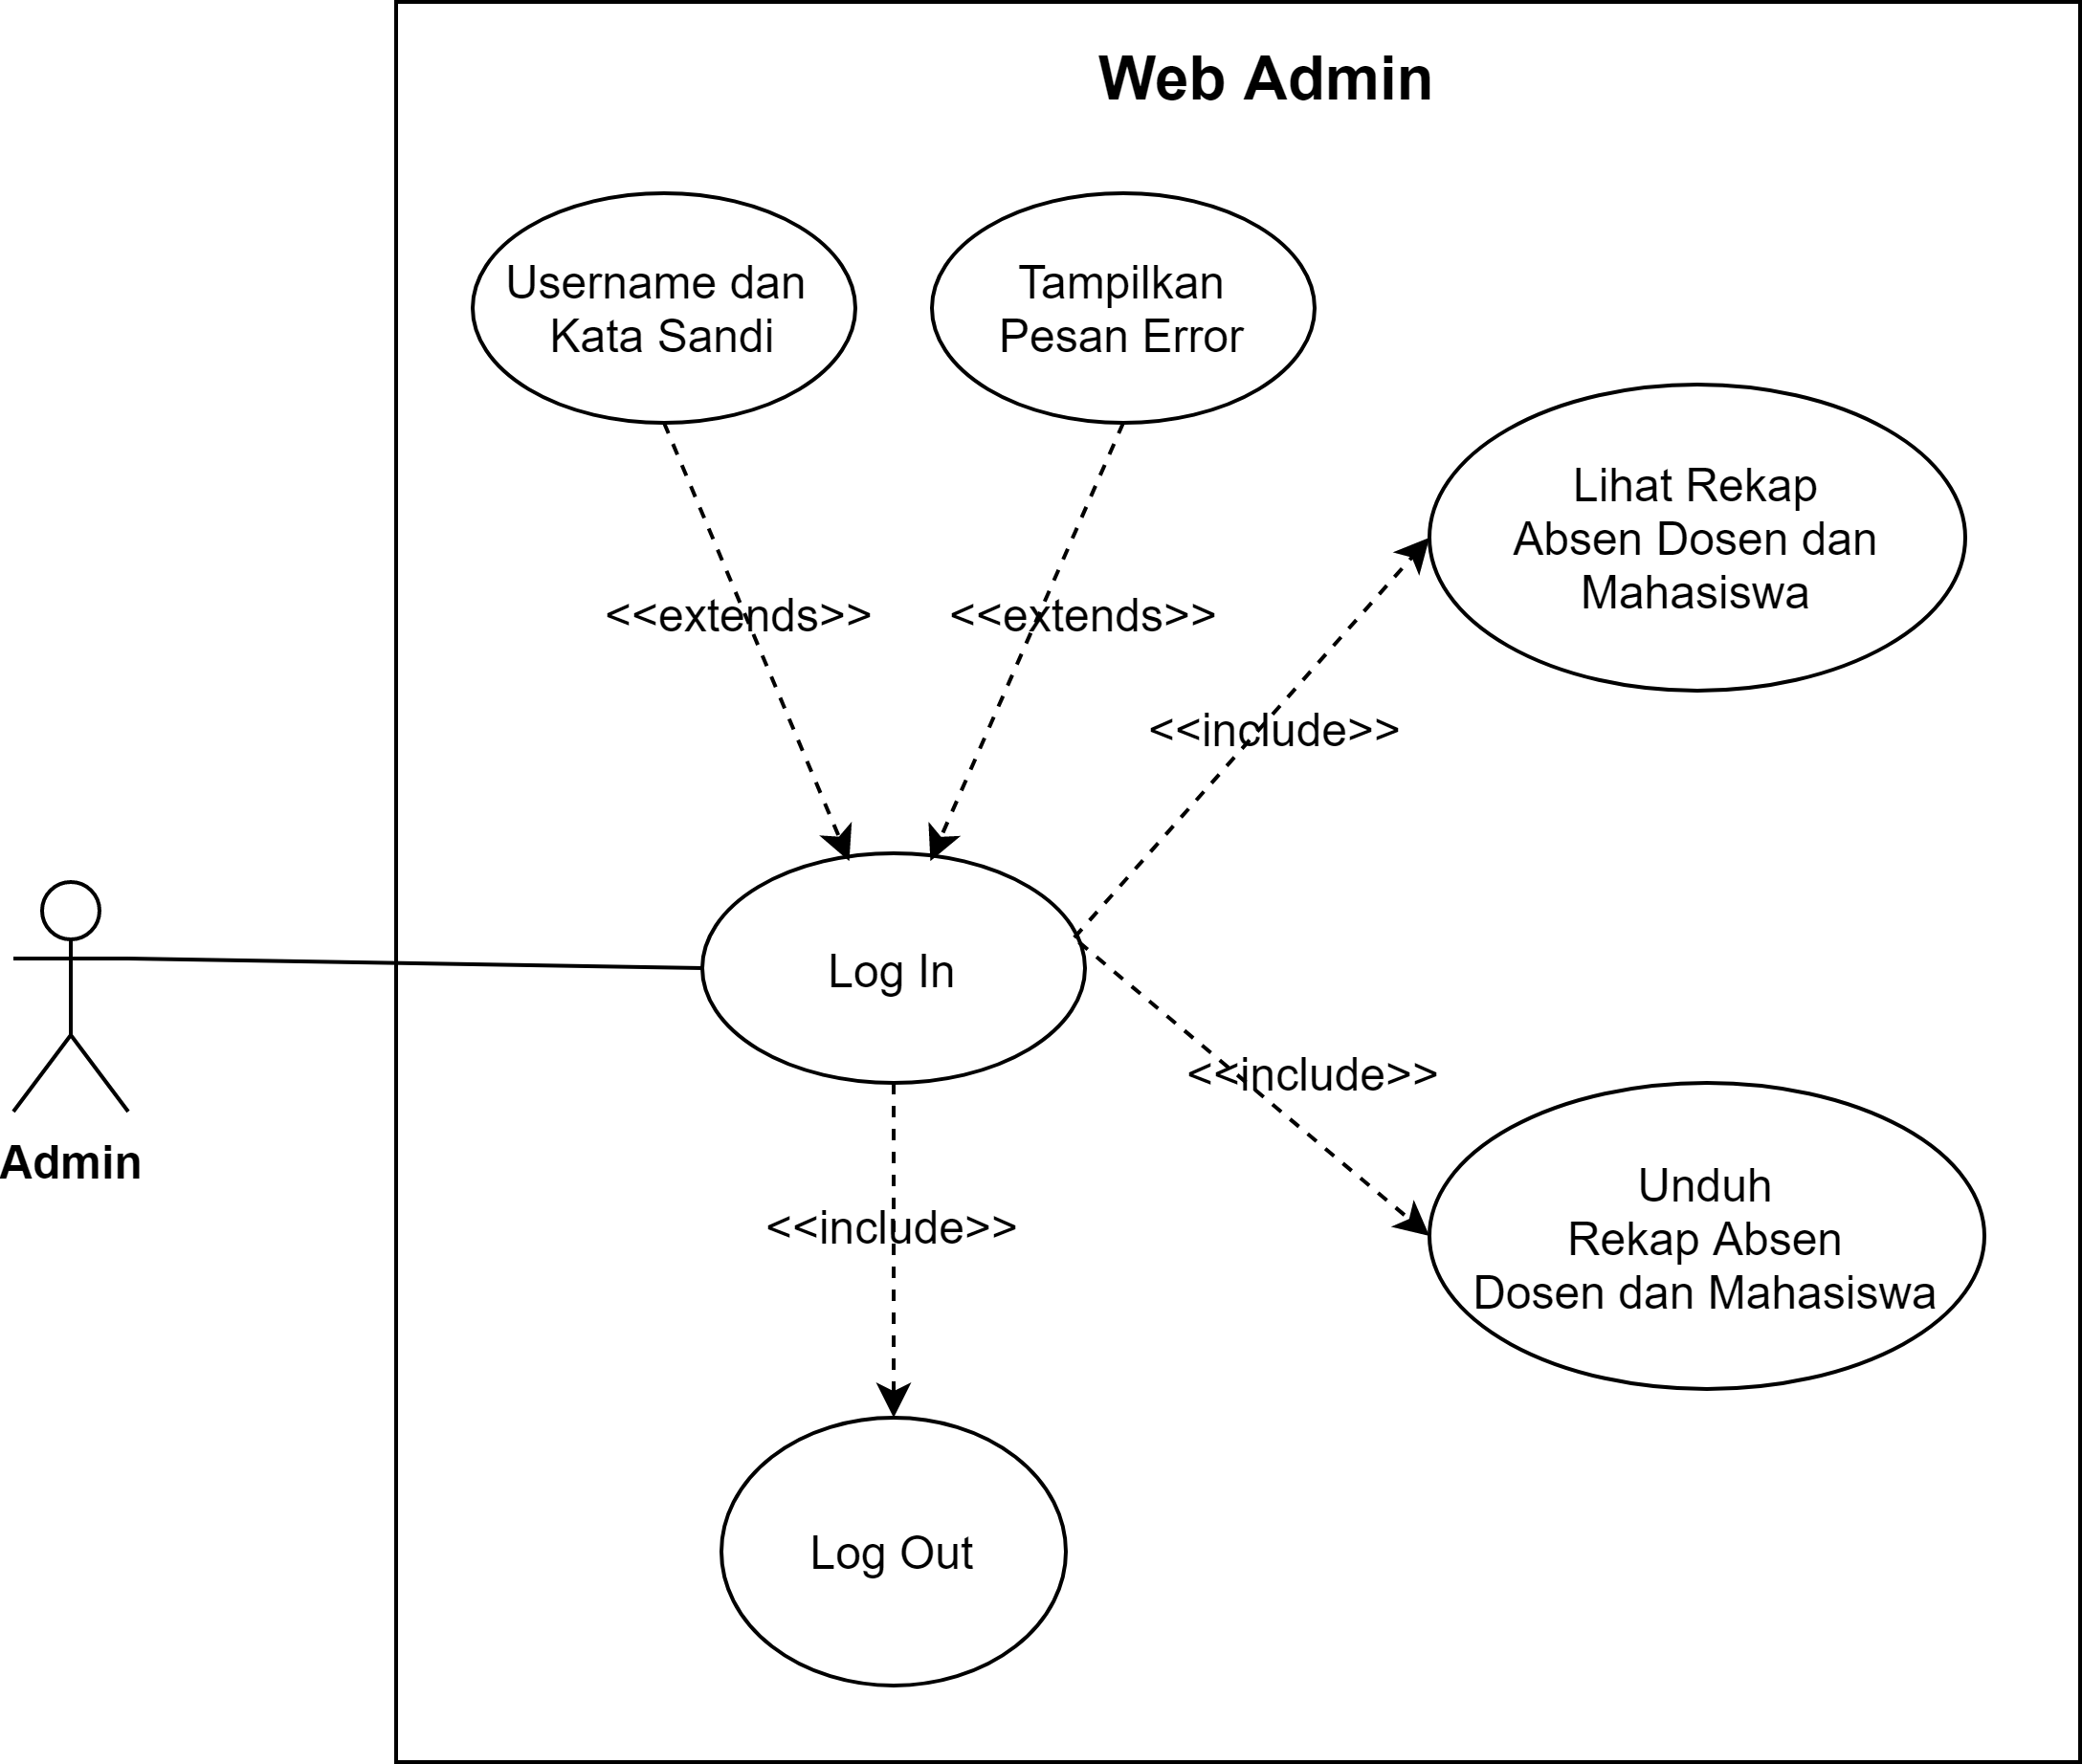
\includegraphics [width=9cm, height=8cm]{gambar/model/use-case-admin}}
		\caption{\textit{Use Case Diagram} Aplikasi Rekap Kehadiran Dosen dan Mahasiswa (Web-Based).}
		\label{usecaseadmin}
	\end{figure}
	
\par Gambar \ref{usecaseadmin} diatas menjelaskan aktivitas yang dapat dilakukan oleh admin saat menggunakan aplikasi. Aktivitas pertama yang dilakukan adalah melakukan \textit{log in} ke aplikasi dengan memasukkan \textit{username} dan kata sandi. Setelah melakukan \textit{log in}, admin dapat melihat daftar kehadiran dosen dan mahasiswa pada mata kuliah tertentu. Selain itu, admin juga dapat mengunduh data-data kehadiran tersebut.
	


	\section{\uppercase{PERANCANGAN DAN PEMBUATAN SISTEM}}
	
	\subsection{Perancangan Sistem}
	\par Perancangan sistem merupakan tahapan proses desain dari sistem perangkat lunak yang dibuat. Proses ini terdiri dari dua tahap yaitu perancangan konfigurasi eksekusi sistem dalam bentuk \textit{deployment diagram} dan perancangan tampilan antar muka (\textit{interface}).
	
   	%Tahap pertama adalah merancang \textit{class diagram} yang bertujuan untuk menggambarkan struktur sistem dari segi pendefinisian dari kelas-kelas yang dibuat untuk membangun sistem. Kelas-kelas yang ada pada struktur sistem harus dapat melakukan fungsi-fungsi sesuai dengan kebutuhan sistem. %Berikut rancangan \textit{class diagram} dari sistem yang telah dibangun dapat dilihat pada Gambar:
   			%\begin{enumerate}
     			%\item \textit{Class Diagram} Aplikasi Mapping
					%\vspace{-0.2cm}
					%\begin{figure}[H]
						%\center
						%\includegraphics [width = 14cm]{gambar/model/class-diagram}
						%\caption{Diagram Kelas Model Basis Data }
					%\label{class}
					%\end{figure}
									
     			%\item \textit{Class Diagram} Aplikasi Kehadiran Dosen
     			%\item \textit{Class Diagram} Aplikasi Kehadiran Mahasiswa
   			%\end{enumerate}
 	%Tahap kedua adalah merancang \textit{component diagram}, dimana \textit{component diagram} dibuat untuk menunjukkan organisasi dan ketergantungan diantara kumpulan komponen dalam sebuah sistem, serta pemodelan bagaimana sistem beradaptasi dengan sistem lain. Berikut rancangan \textit{component diagram} dari sistem yang telah dibangun dapat dilihat pada Gambar \ref{componentmapping} dan Gambar \ref{componentabsensi}.
 			%\begin{enumerate}
     			%\item \textit{Component Diagram} Aplikasi Mapping
					%\vspace{-0.2cm}
					%\begin{figure}[H]
						%\center
						%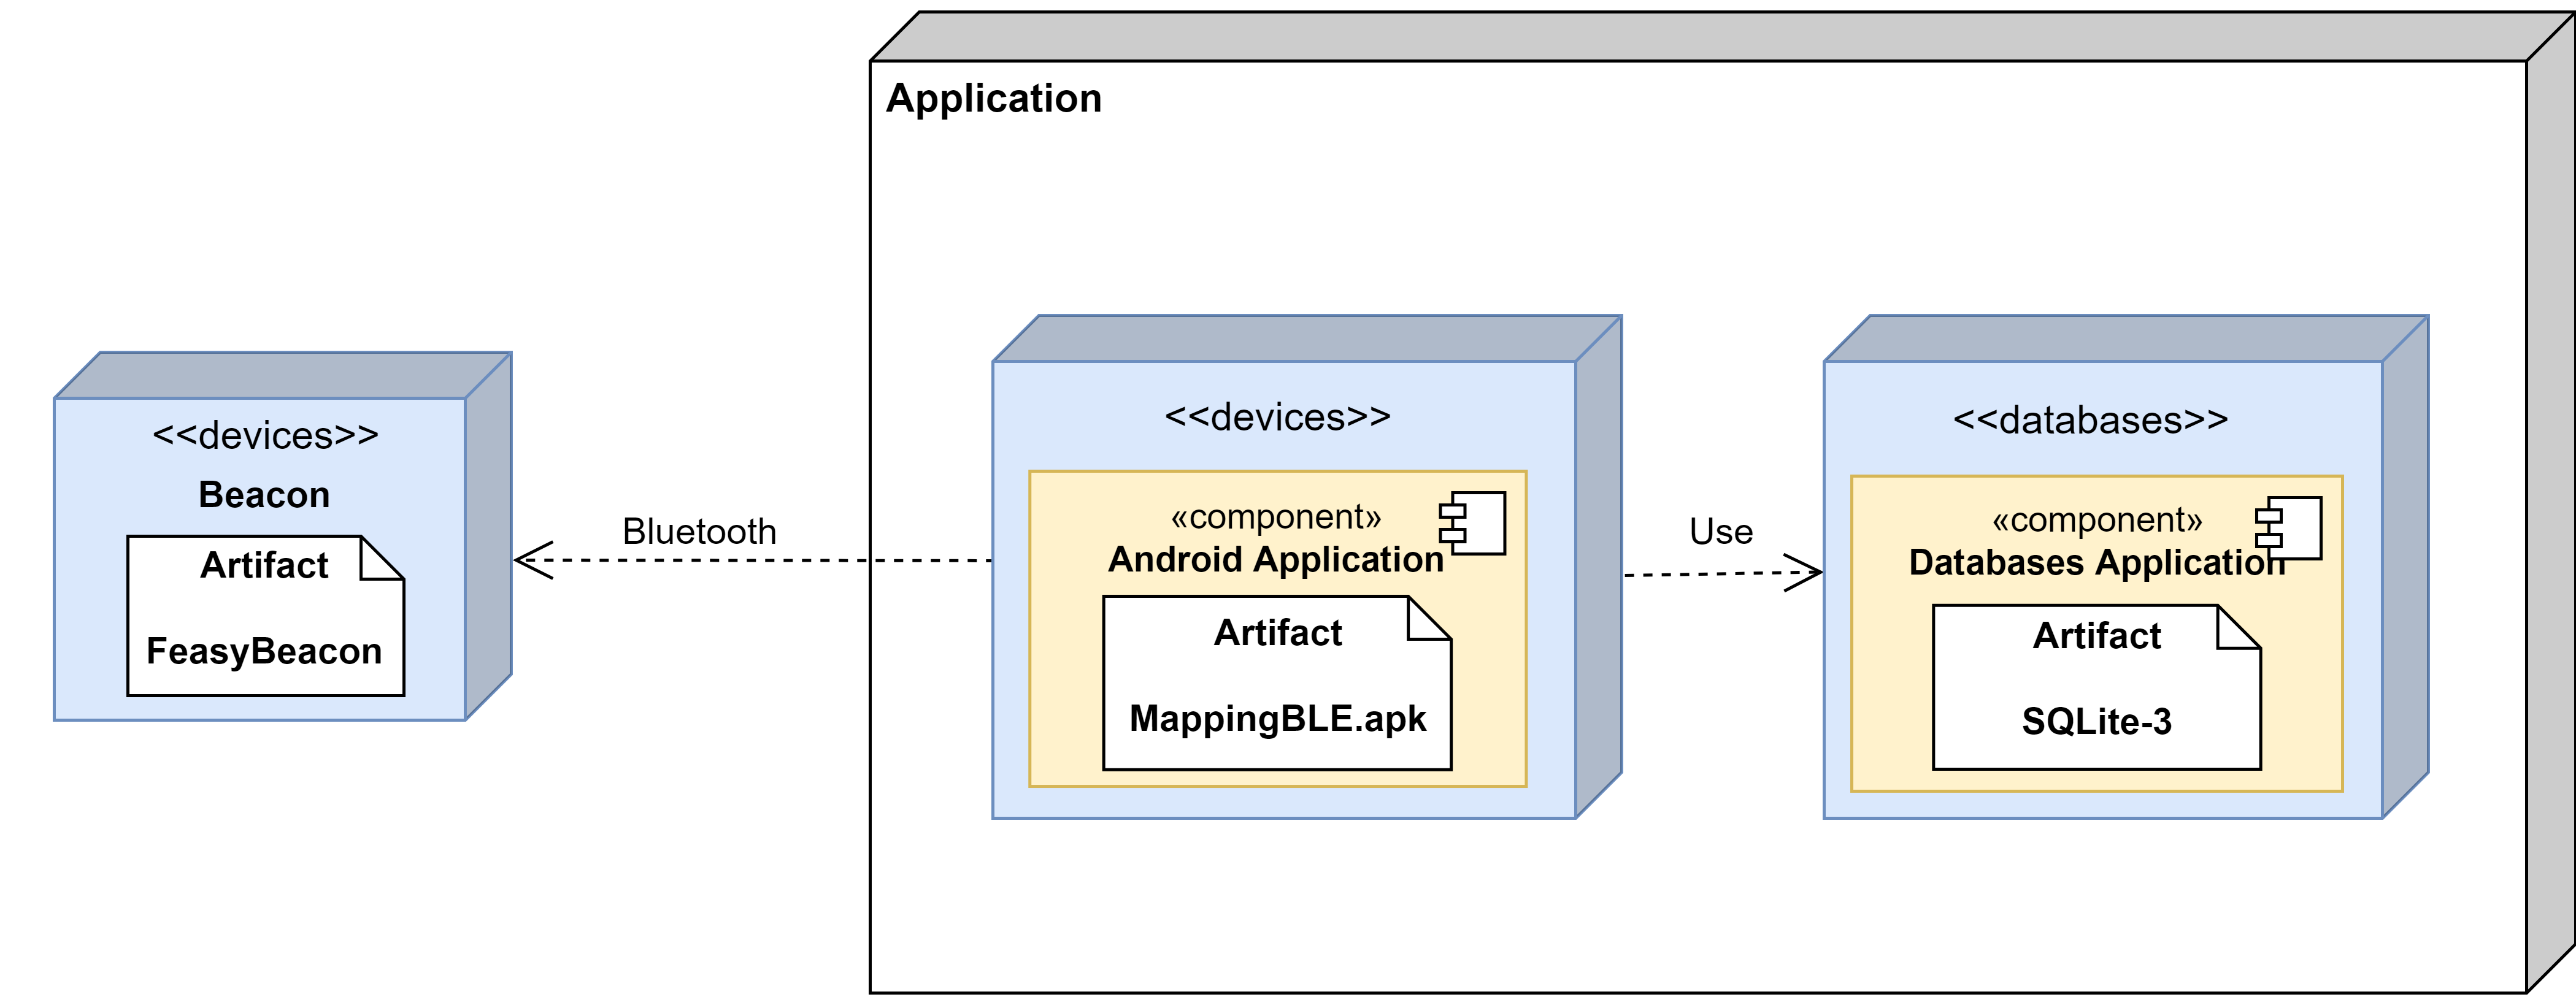
\includegraphics [width = 13cm, height= 5cm]{gambar/model/component-diagram-mapping}
						%\caption{Diagram Component Aplikasi Mapping}
					%\label{componentmapping}
					%\end{figure}
									
     			%\item \textit{Component Diagram} Aplikasi Kehadiran Dosen dan Aplikasi Kehadiran Mahasiswa
     				%\vspace{-0.2cm}
					%\begin{figure}[H]
						%\center
						%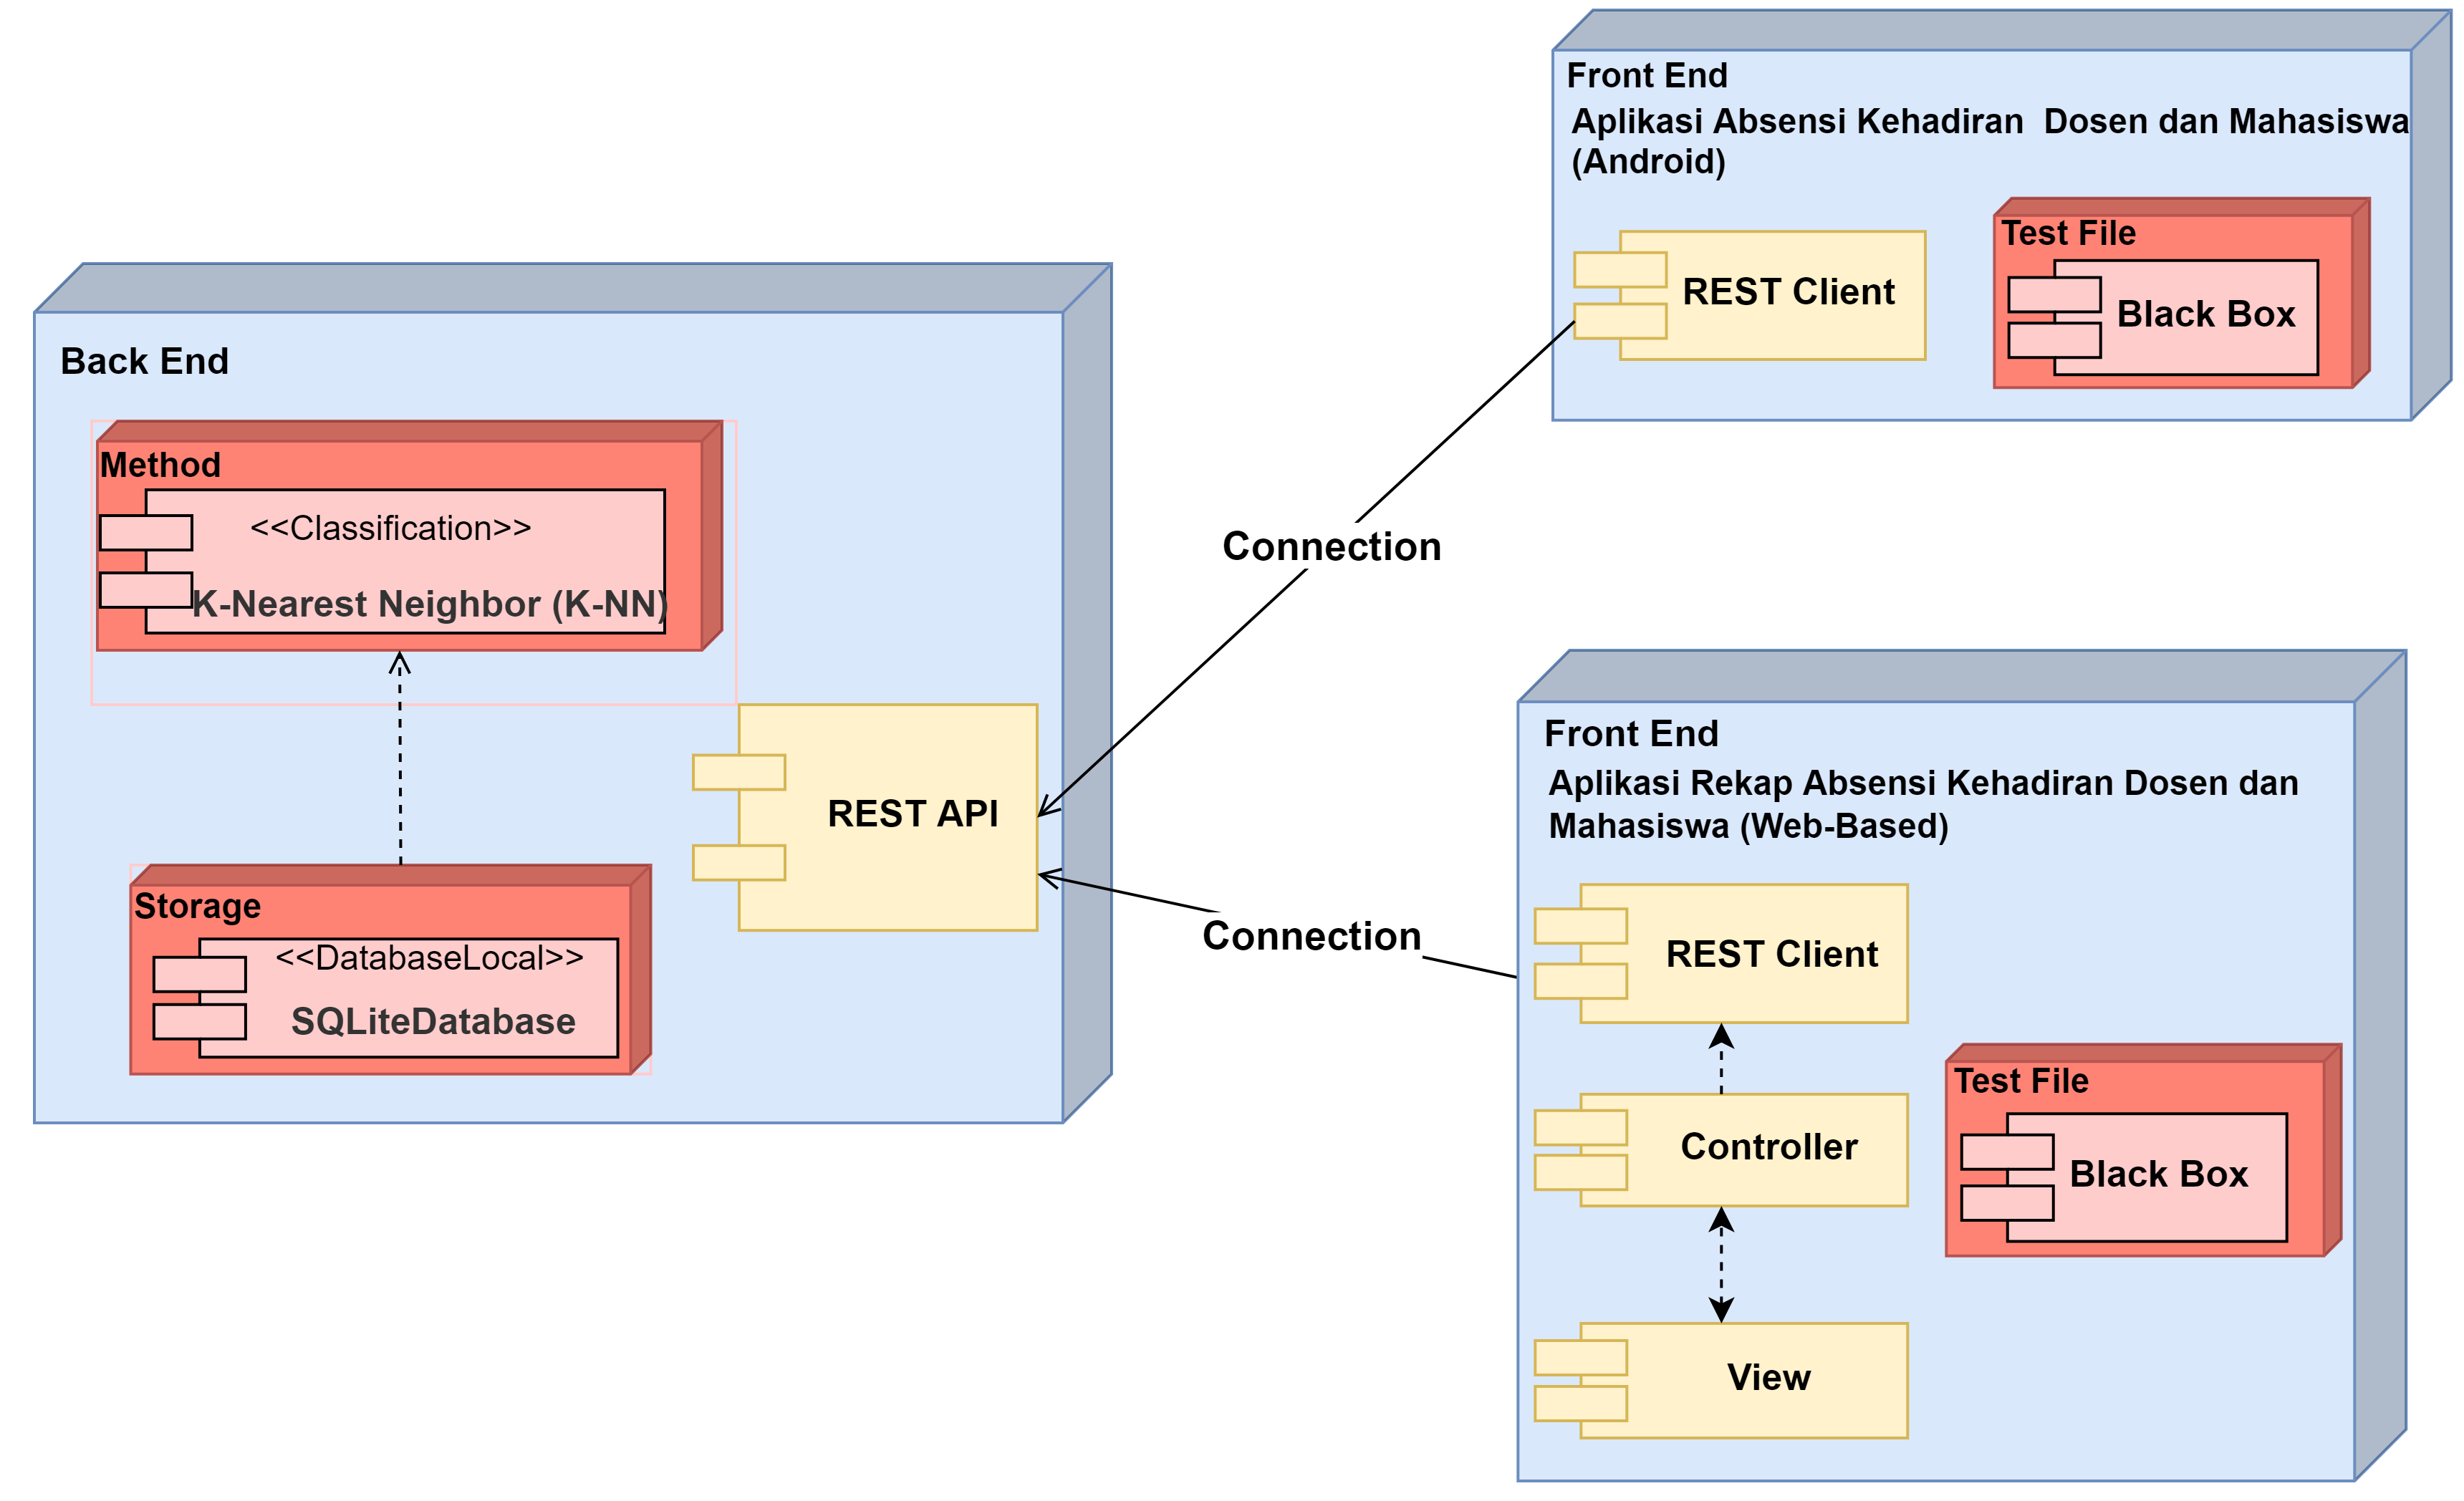
\includegraphics [width = 13.5cm, height= 9cm]{gambar/model/component-diagram-absensi}
						%\caption{Diagram Component Aplikasi Kehadiran Dosen dan Mahasiswa}
					%\label{componentabsensi}
					%\end{figure}
   			%\end{enumerate}
   	Tahap pertama adalah merancang \textit{deployment diagram}, dimana \textit{deployment diagram} adalah diagram yang menjelaskan bagaimana sistem bekerja dan digunakan oleh pengguna. Berikut rancangan \textit{deployment diagram} dari sistem yang telah dibangun dapat dilihat pada Gambar \ref{deployment-diagram}.
   		
 			%\begin{enumerate}
     			%\item \textit{Deployment Diagram} Aplikasi Mapping
					\vspace{-0.2cm}
				 \begin{landscape}
					\begin{figure}[H]
						\center
						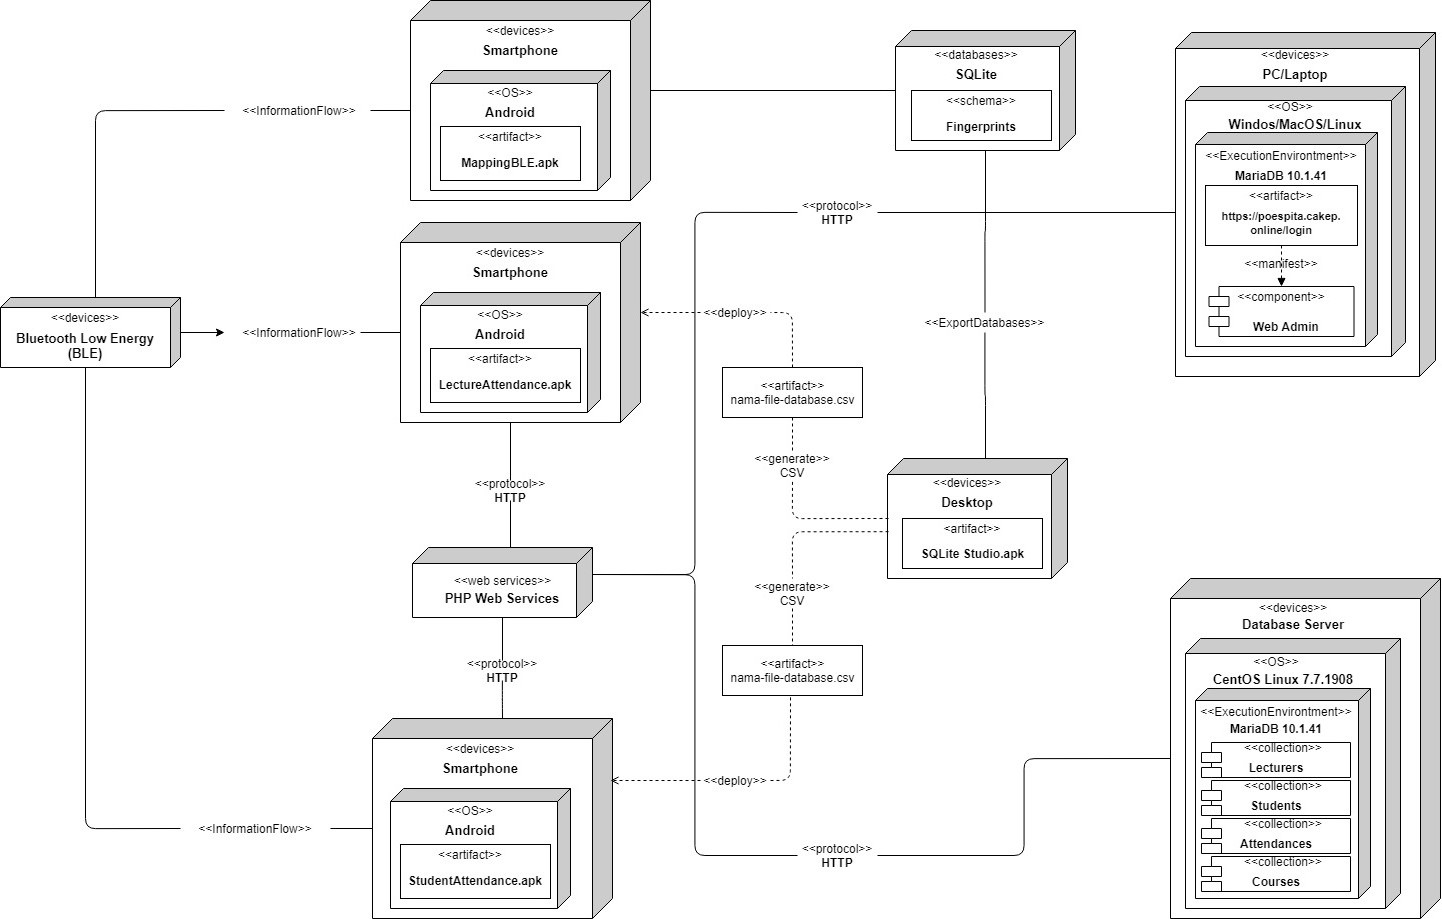
\includegraphics [width = 22.5cm, height=12cm]{gambar/model/deployment-diagram}
						\caption{Diagram \textit{Deployment}}
					\label{deployment-diagram}
					\end{figure}
				  \end{landscape}
									
     			%\item \textit{Deployment Diagram} Aplikasi Kehadiran Dosen dan Aplikasi Kehadiran Mahasiswa
     				%\vspace{-0.2cm}
					%\begin{figure}[H]
						%\center
						%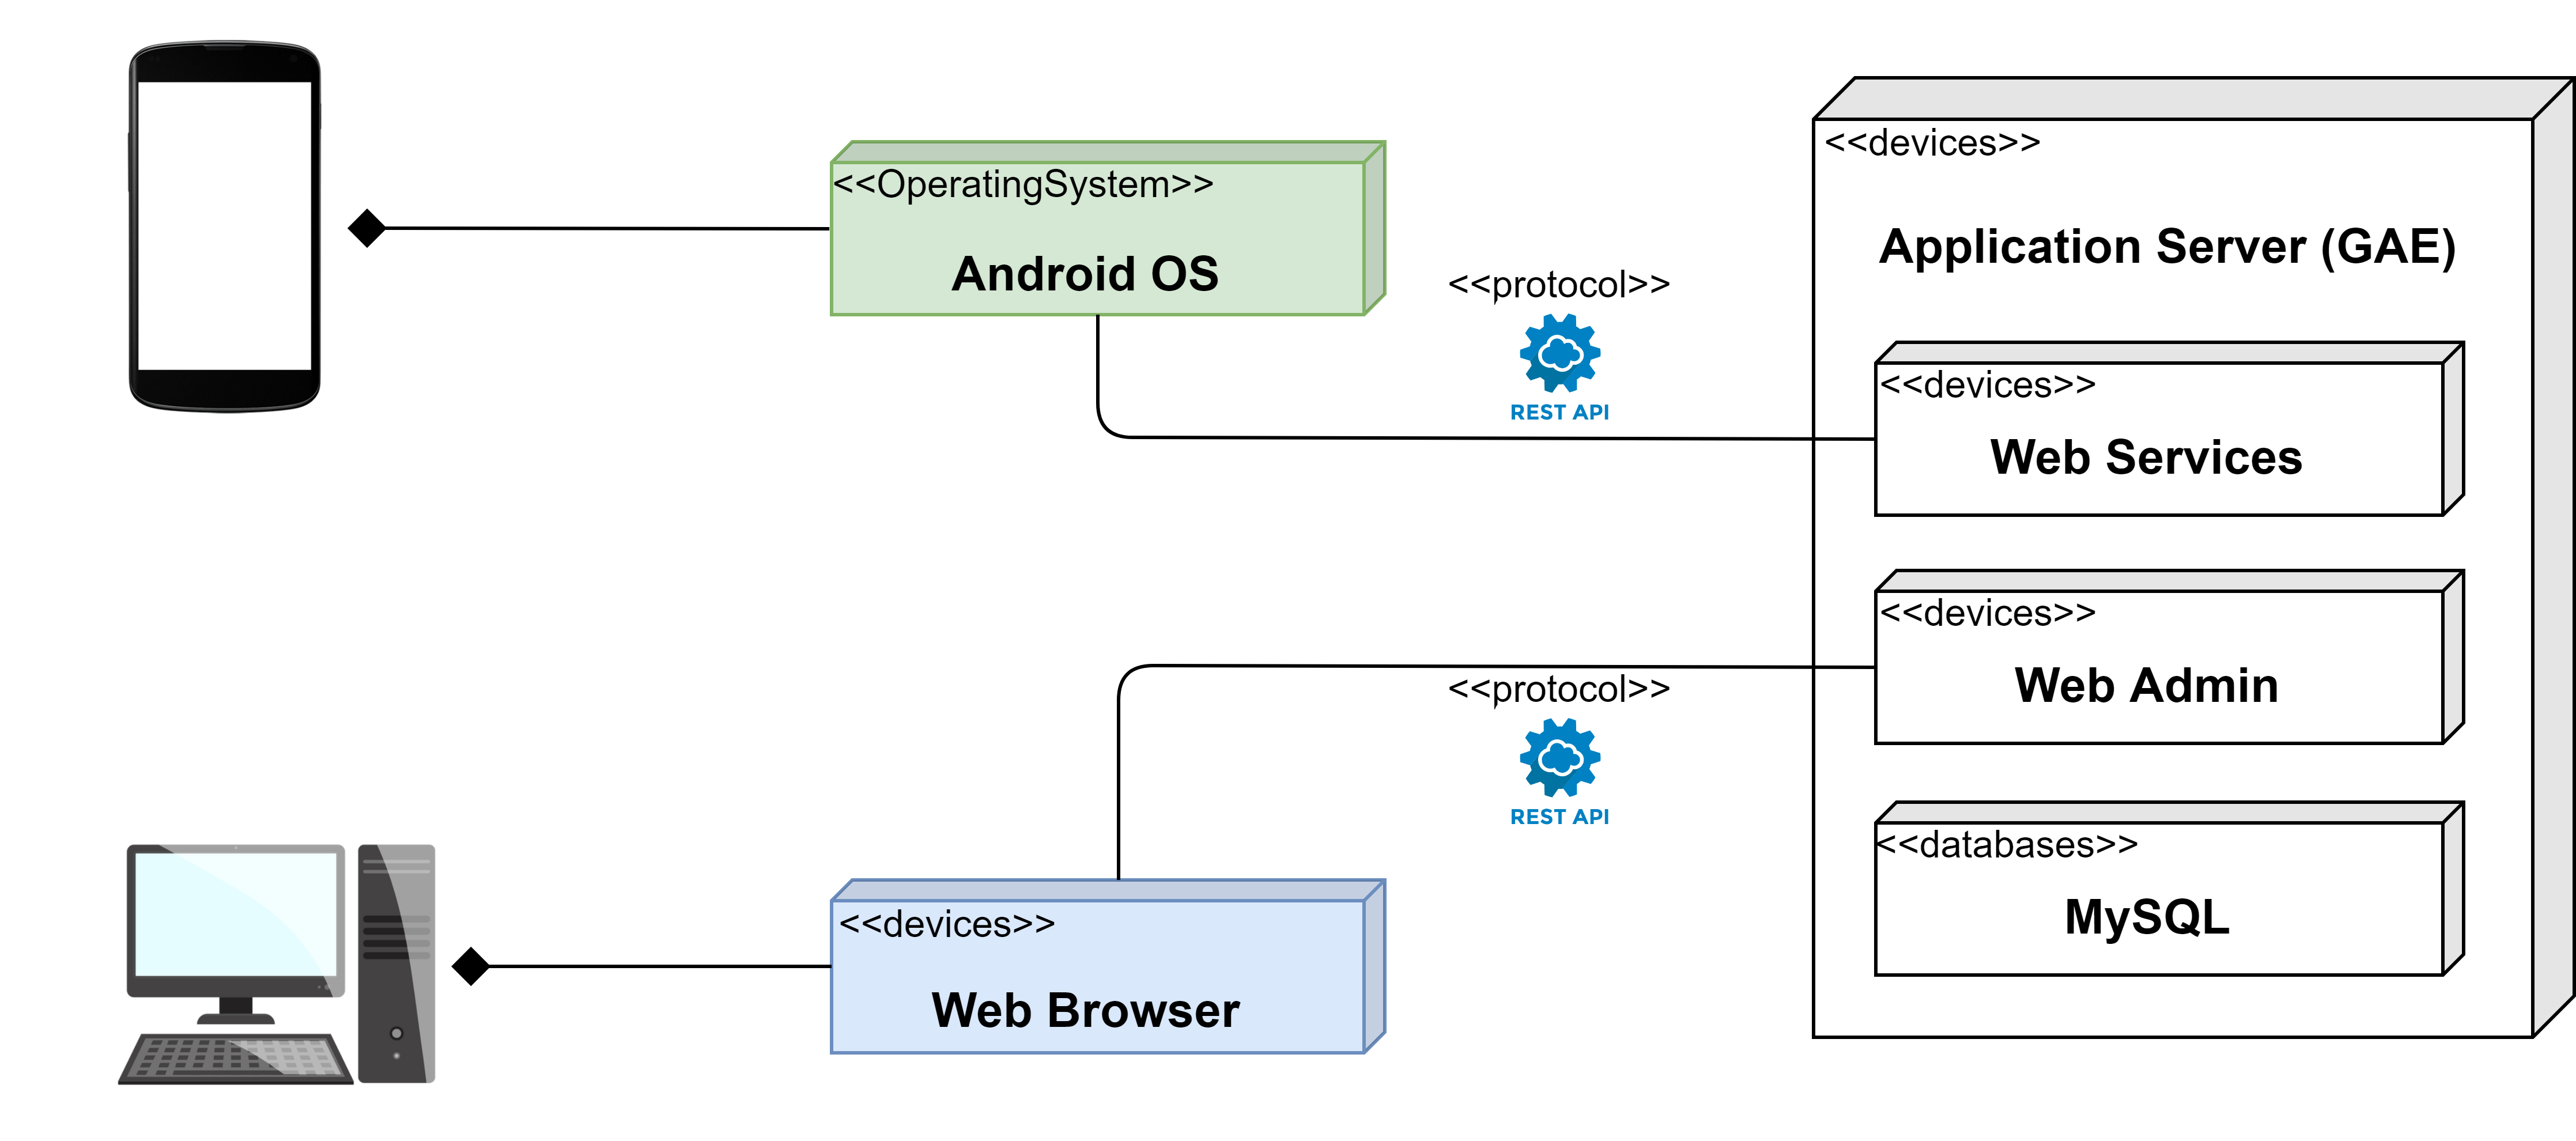
\includegraphics [width = 13.5cm, height= 5.5cm]{gambar/model/deployment-diagram-absensi}
						%\caption{Diagram Deployment Aplikasi Kehadiran Dosen dan Mahasiswa}
					%\label{deploymentabsensi}
					%\end{figure}
   			%\end{enumerate}
 	
	Tahap kedua adalah merancang tampilan antar muka pengguna (\textit{user interface}) sebagai mekanisme komunikasi dengan sistem. Antar muka dari sistem yang telah dibangun adalah sebagai berikut:
		\begin{enumerate}[a.]
		
		\item Antar Muka Aplikasi Mapping
		
		\par Gambar \ref{aplikasimappingbagian1} menampilkan halaman ketika menggunakan aplikasi, kemudian akan muncul notifikasi permintaan izin mengakses lokasi pada perangkat untuk pemindaian kekuatan sinyal Bluetooth. Halaman beranda menampilkan informasi nama ruangan, nama \textit{device} Bluetooth, RSSI dan MAC Address Bluetooth apabila proses pemindaian telah selesai dilakukan serta beberapa tombol untuk memulai proses pemindaian, tombol untuk menyimpan data hasil pemindaian, dan tombol untuk menampilkan data hasil pemindaian.  
				
		\vspace{-0cm}
	\begin{figure} [H]
	\begin{subfigure}{.5\textwidth}
  		\centering
  		% include first image
  		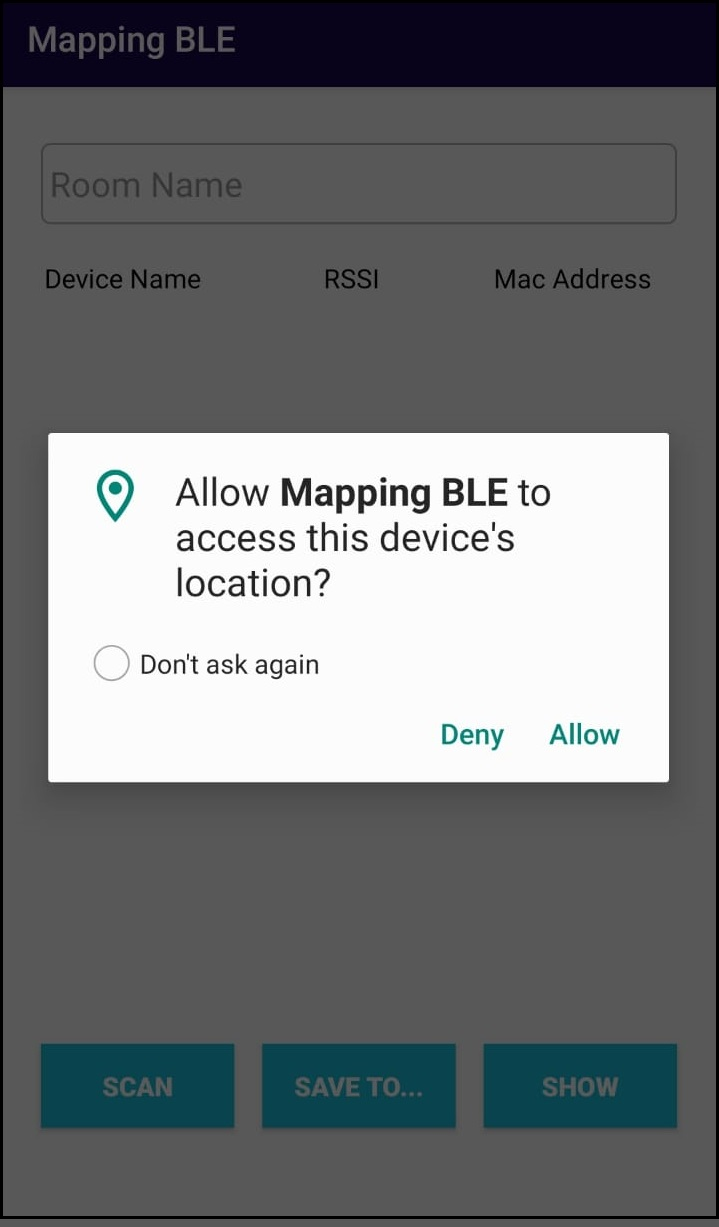
\includegraphics[width=.5\linewidth]{gambar/android/mapping-permission}  
  		\caption{Izin mengakses lokasi}
	\end{subfigure}
	\begin{subfigure}{.5\textwidth}
  		\centering
  		% include second image
		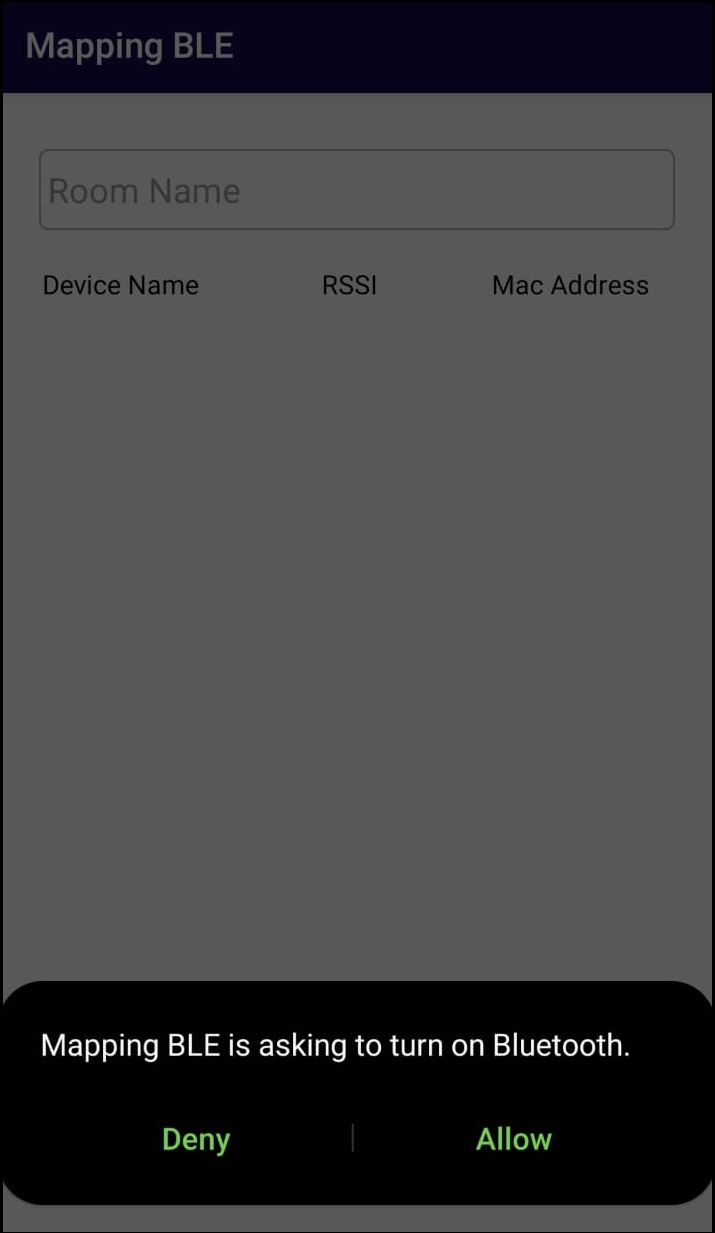
\includegraphics[width=.5\linewidth]{gambar/android/mapping-bluetooth}  
  		\caption{Menghidupkan Bluetooth}
	\end{subfigure}
		\vspace{1cm}
		\newline
	\begin{subfigure}{.5\textwidth}
  		\centering
		 % include third image
	  	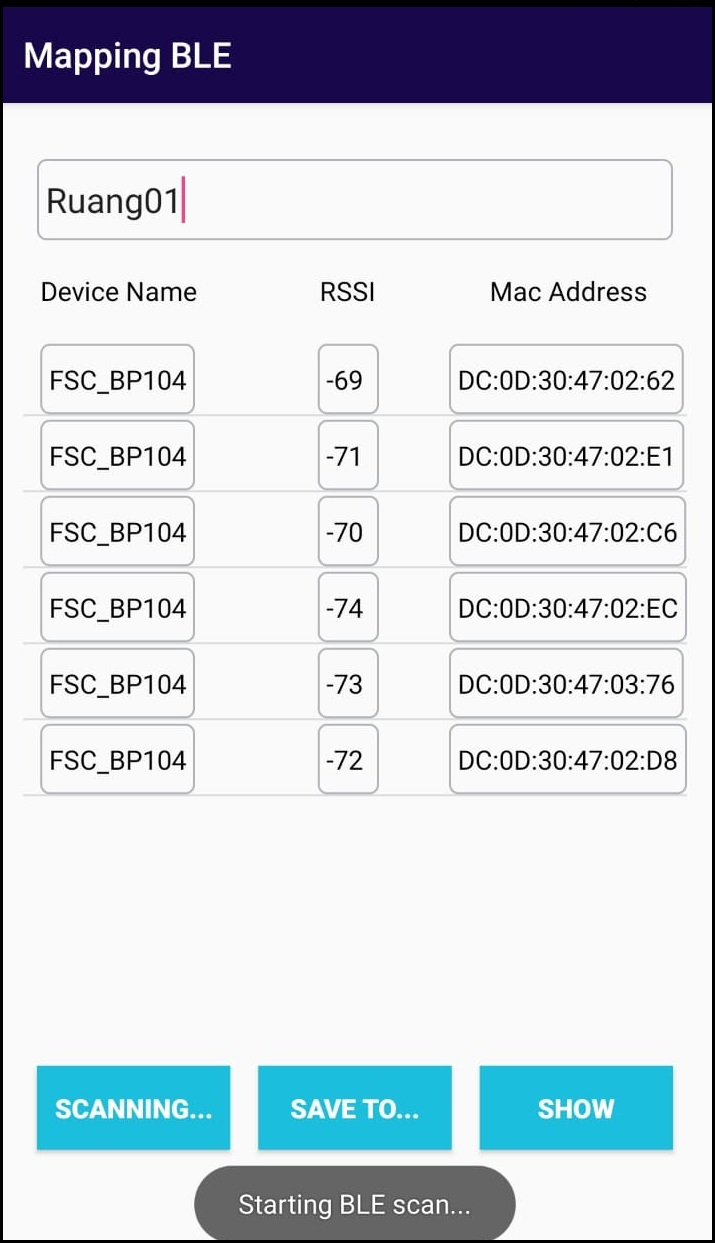
\includegraphics[width=.5\linewidth]{gambar/android/mapping-scanning}  
  		\caption{Proses pemindaian kekuatan sinyal}
	\end{subfigure}
	\begin{subfigure}{.5\textwidth}
  		\centering
  		% include fourth image
  		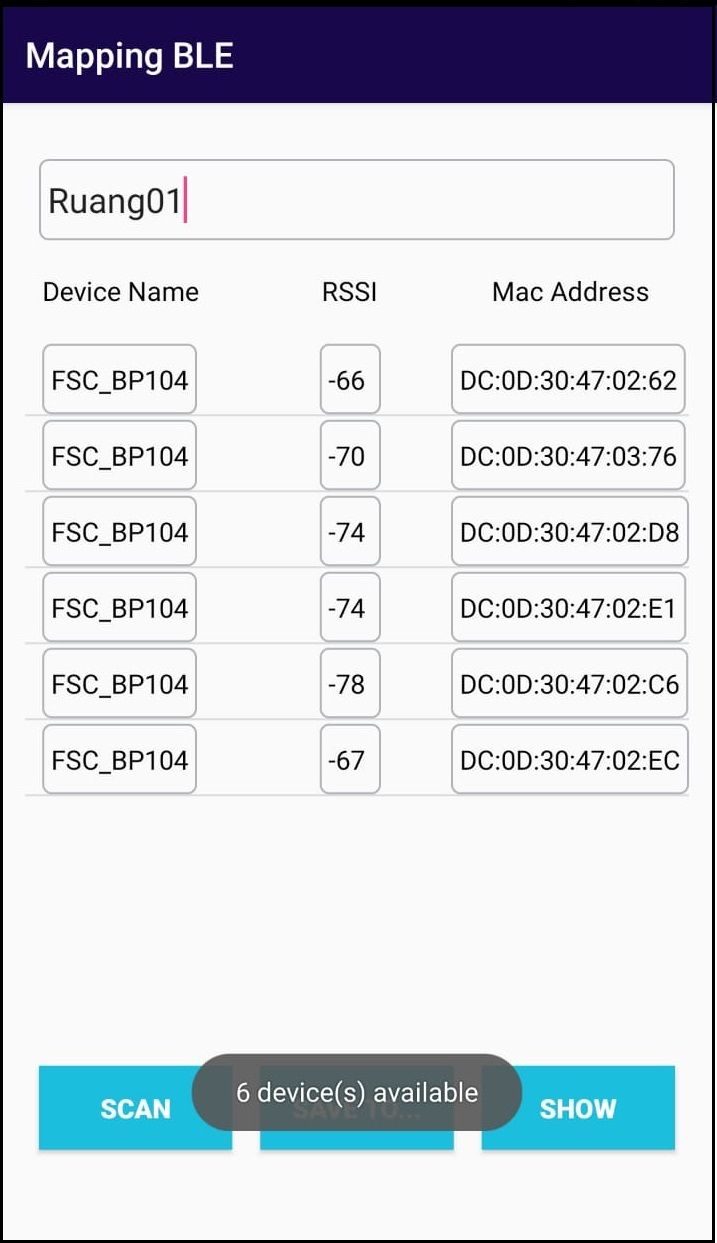
\includegraphics[width=.5\linewidth]{gambar/android/mapping-finish-scan}  
  		\caption{Selesai proses pemindaian}
	\end{subfigure}
		\vspace{0.5cm}
		\caption{Tampilan Halaman Aplikasi Mapping (Bagian 1)}
	\label{aplikasimappingbagian1}
	\end{figure}
	
	\par Apabila pengguna menekan tombol \textbf{save to}, akan muncul \textit{pop up} dimana pengguna dapat memilih tabel penyimpanan data hasil pemindaian, yaitu: tabel \textit{reference point} urut dan tabel \textit{reference point} acak. Jika pengguna menekan tombol \textbf{show data}, akan muncul \textit{pop up} dimana pengguna dapat memilih tabel untuk data yang ingin ditampilkan, kemudian pengguna akan diarahkan ke halaman daftar data hasil pemindaian kekuatan sinyal yang telah disimpan sebelumnya. Jika pengguna ingin menghapus sebuah data, pengguna harus menekan tombol \textit{icon} tong sampah dan lakukan konfirmasi. Fitur-fitur tersebut dapat dilihat pada Gambar \ref{aplikasimappingbagian2}.   
	
	\vspace{-0cm}
	\begin{figure} [H]
	\begin{subfigure}{.5\textwidth}
  		\centering
  		% include first image
  		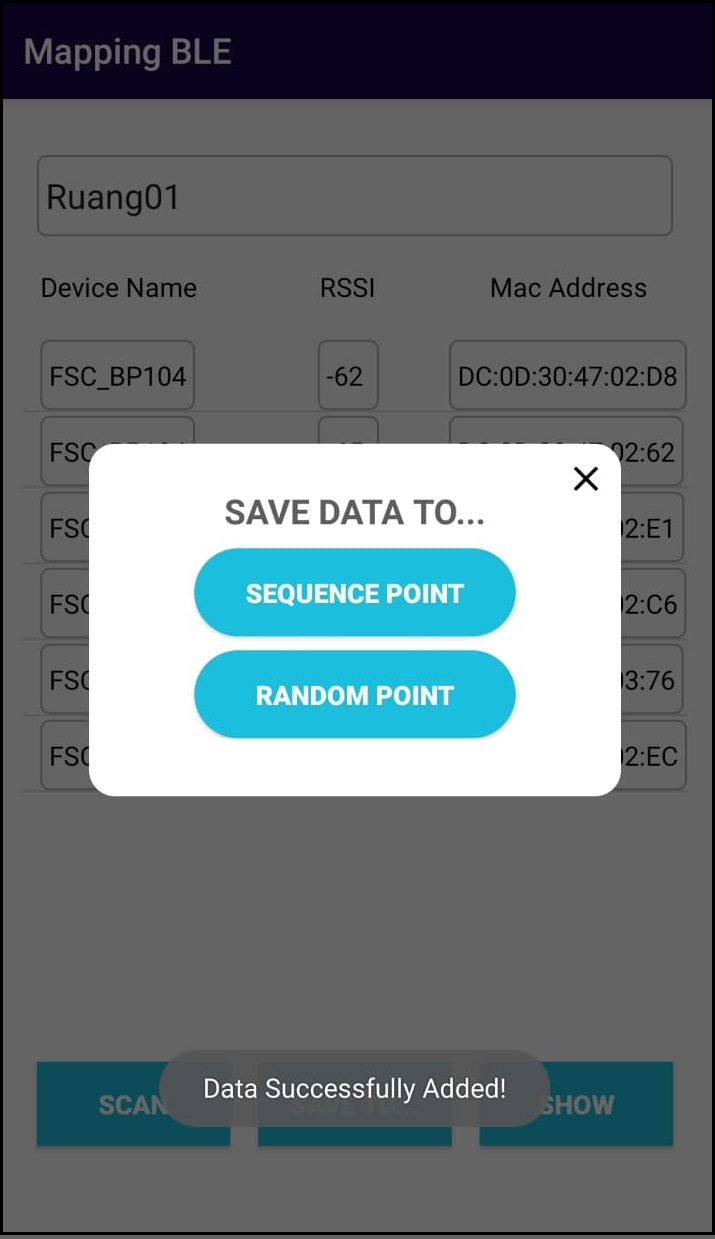
\includegraphics[width=.5\linewidth]{gambar/android/mapping-save-data}  
  		\caption{Simpan hasil pemindaian}
	\end{subfigure}
	\begin{subfigure}{.5\textwidth}
  		\centering
  		% include second image
  		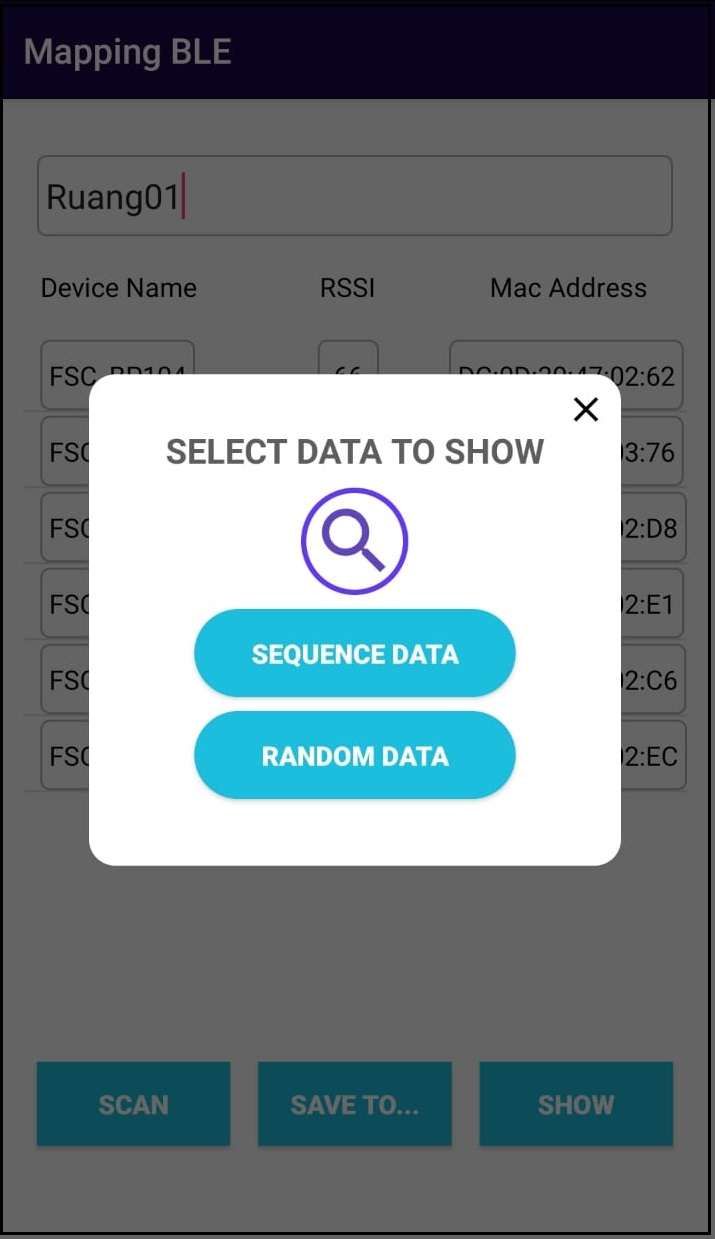
\includegraphics[width=.5\linewidth]{gambar/android/mapping-show-data}  
  		\caption{Pilihan menampilkan data}
	\end{subfigure}
	\vspace{1cm}
	\newline
	\begin{subfigure}{.5\textwidth}
  		\centering
  		% include third image
  		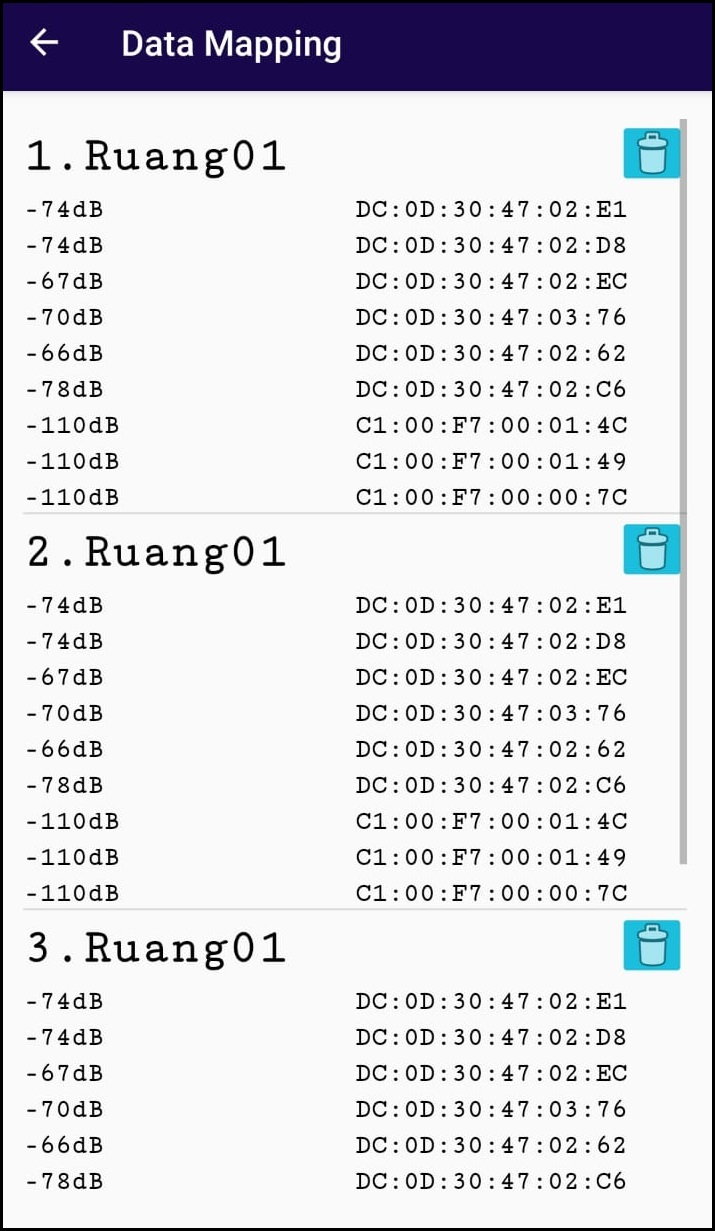
\includegraphics[width=.5\linewidth]{gambar/android/mapping-data-list}  
  		\caption{Menampilkan data yang disimpan}
	\end{subfigure}
	\begin{subfigure}{.5\textwidth}
  		\centering
  		% include fourth image
  		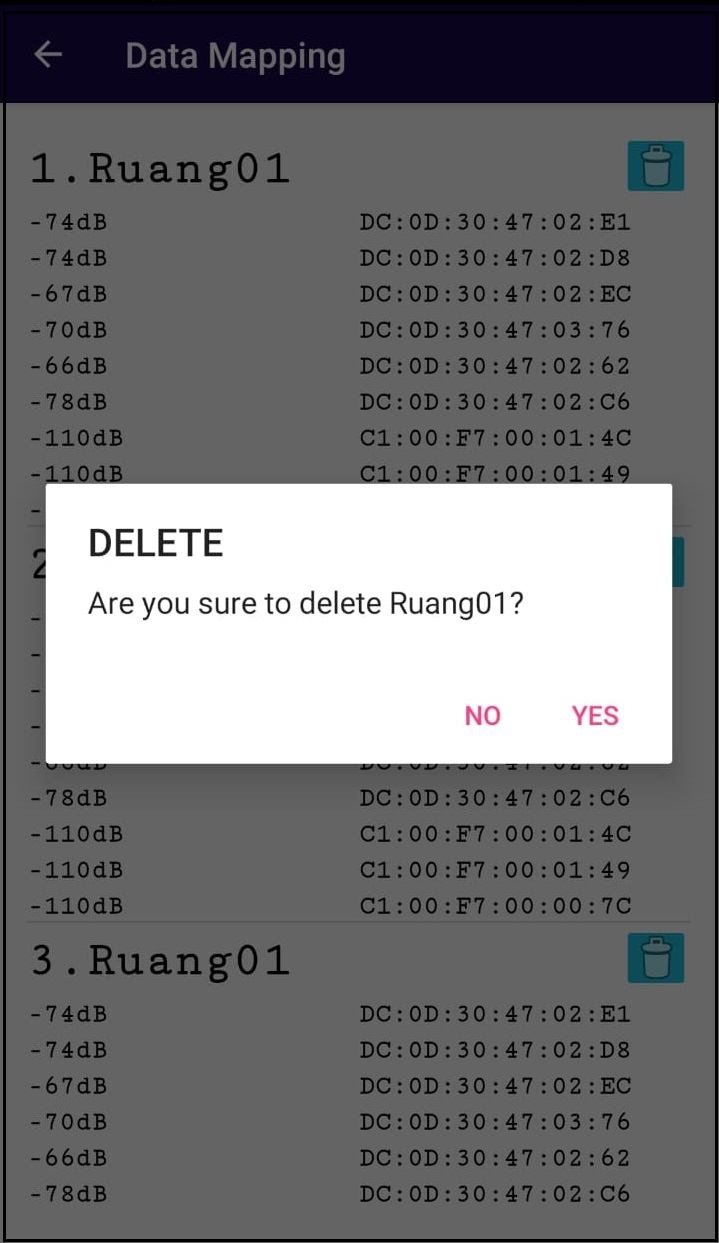
\includegraphics[width=.5\linewidth]{gambar/android/mapping-delete}
  		\caption{Hapus data}
	\end{subfigure}
		\vspace{0.5cm}
		\caption{Tampilan Halaman Aplikasi Mapping (Bagian 2)}
	\label{aplikasimappingbagian2}
	\end{figure}
	%Akhir Gambar Aplikasi Mapping%
	
\vspace{1cm}
		\item Antar Muka Aplikasi Kehadiran Dosen
		
		\par Gambar \ref{aplikasidosenbagian1} memperlihatkan ketika dosen belum melakukan \textit{log in}, aplikasi akan menampilkan \textit{landing page} yang berisi langkah-langkah penggunaan aplikasi, selanjutnya dosen akan diarahkan ke halaman \textit{log in}. Untuk melakukan \textit{log in}, dosen diminta untuk memasukkan Nomor Induk Pegawai (NIP) dan kata sandi yang sesuai dengan Sistem Kepegawaian (SIMPEG) Unsyiah. Setelah itu, dosen akan diarahkan ke halaman beranda apabila telah berhasil melakukan \textit{log in}. Pada halaman beranda, terdapat informasi data diri dosen serta mata kuliah yang diajarkan oleh dosen yang bersangkutan. Jika dosen menekan salah-satu mata kuliah, dosen akan diarahkah ke halaman informasi mata kuliah tersebut.
	\vspace{-0cm}
	\begin{figure} [H]
	\begin{subfigure}{.5\textwidth}
  		\centering
  		% include first image
  		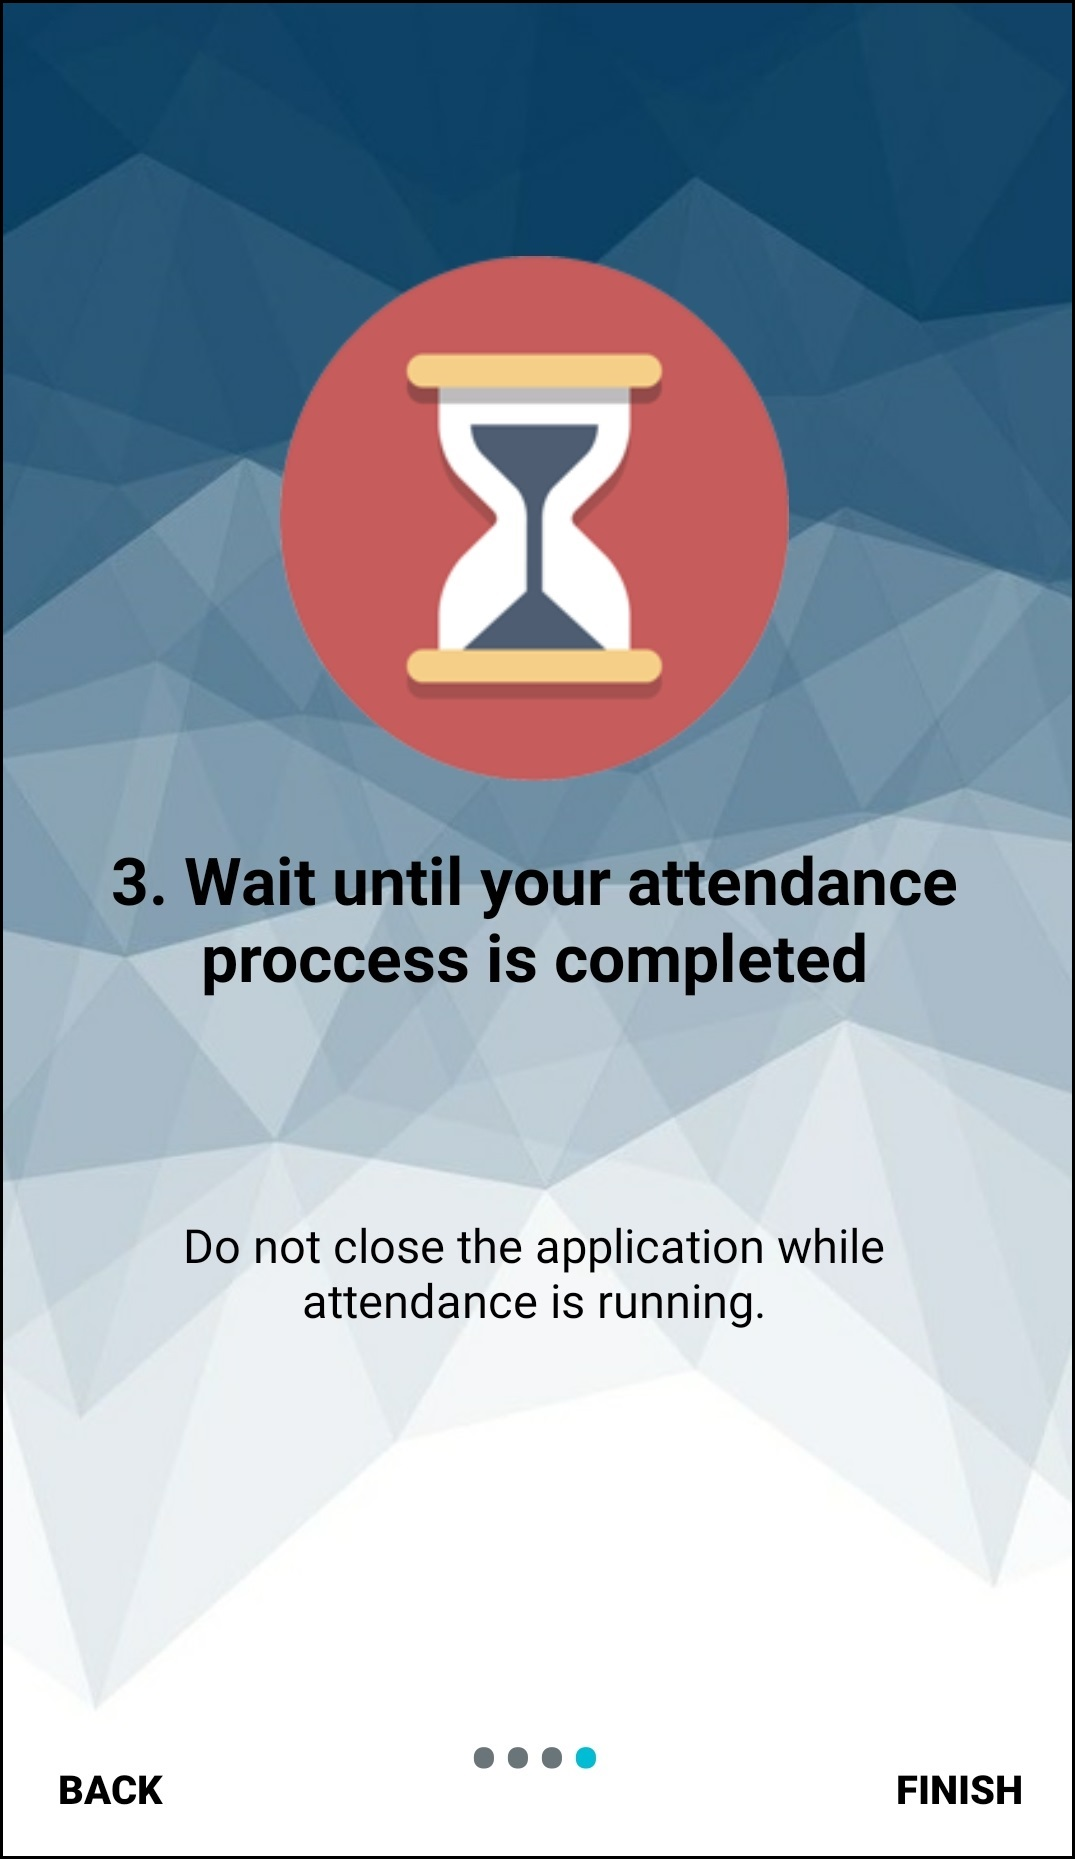
\includegraphics[width=.5\linewidth]{gambar/android/dosen-1}  
  		\caption{\textit{Landing page}}
	\end{subfigure}
	\begin{subfigure}{.5\textwidth}
  		\centering
  		% include second image
		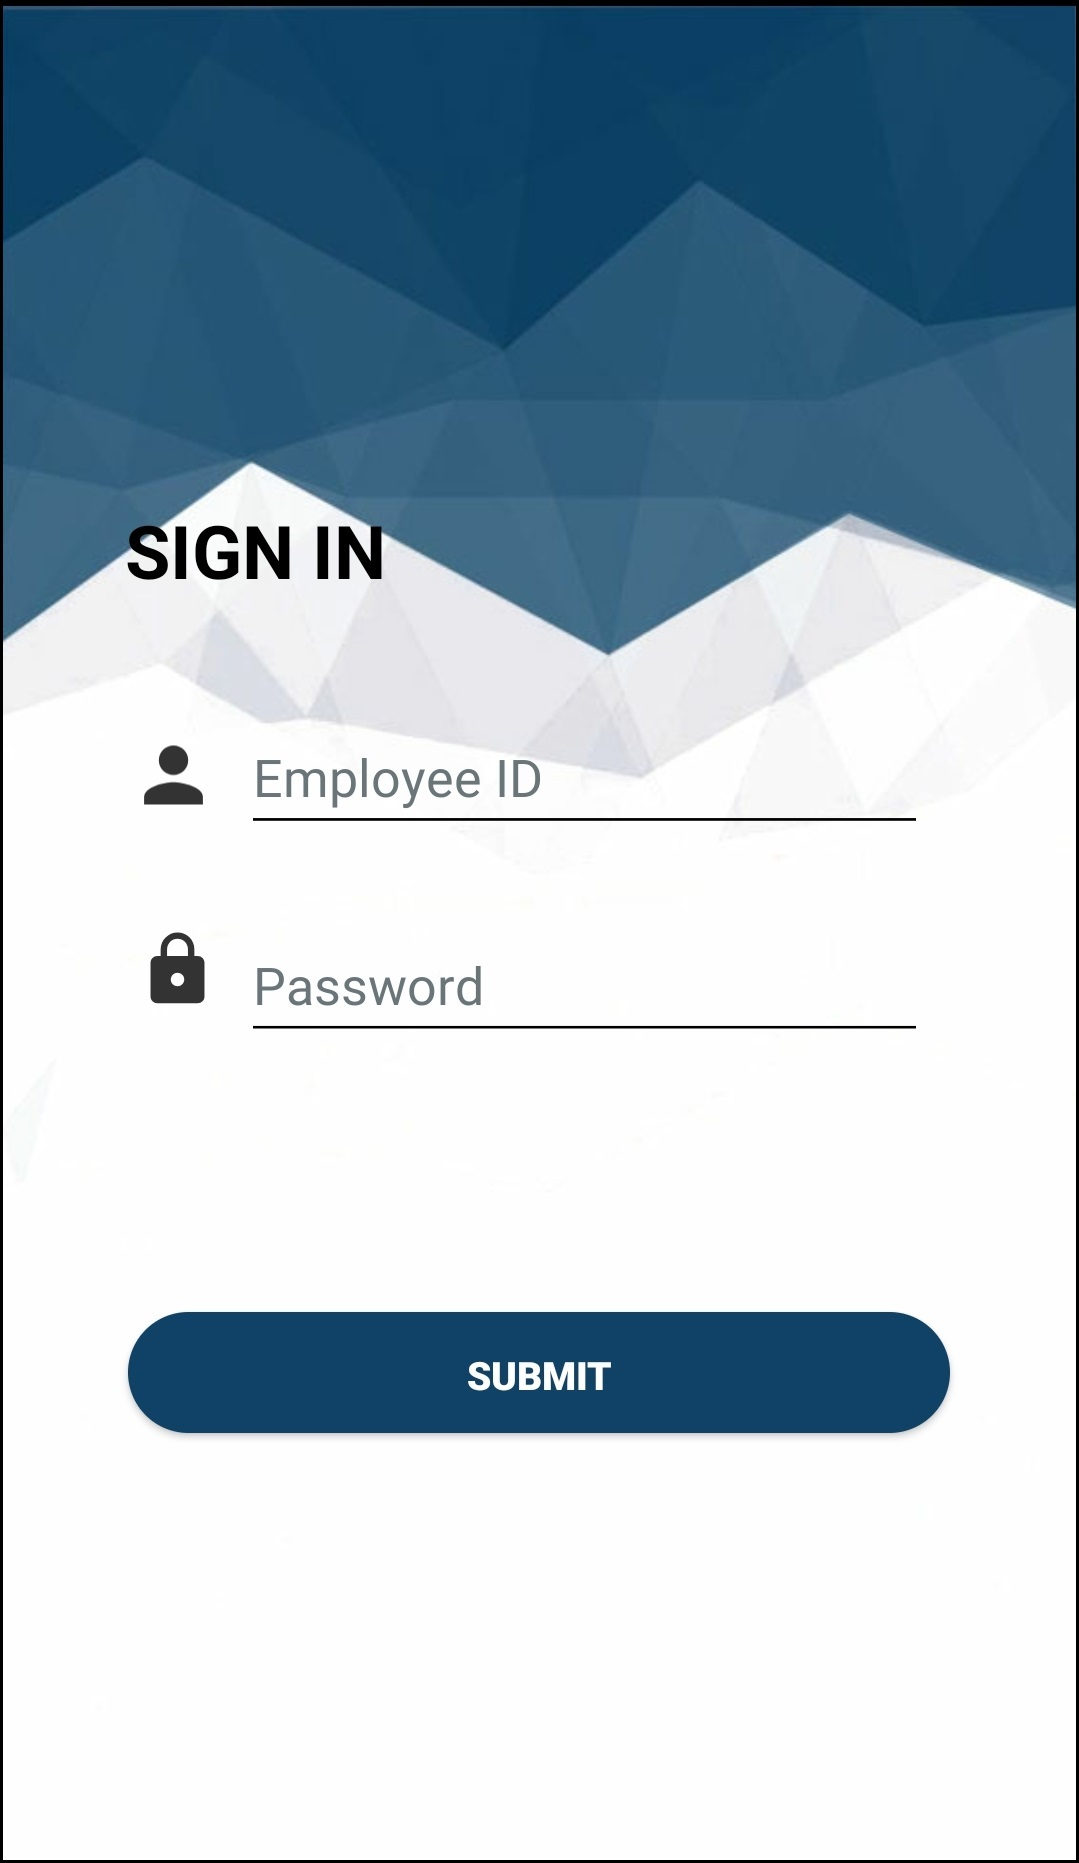
\includegraphics[width=.5\linewidth]{gambar/android/dosen-2}  
  		\caption{\textit{Log in}}
	\end{subfigure}
		\vspace{1cm}
		\newline
	\begin{subfigure}{.5\textwidth}
  		\centering
		 % include third image
	  	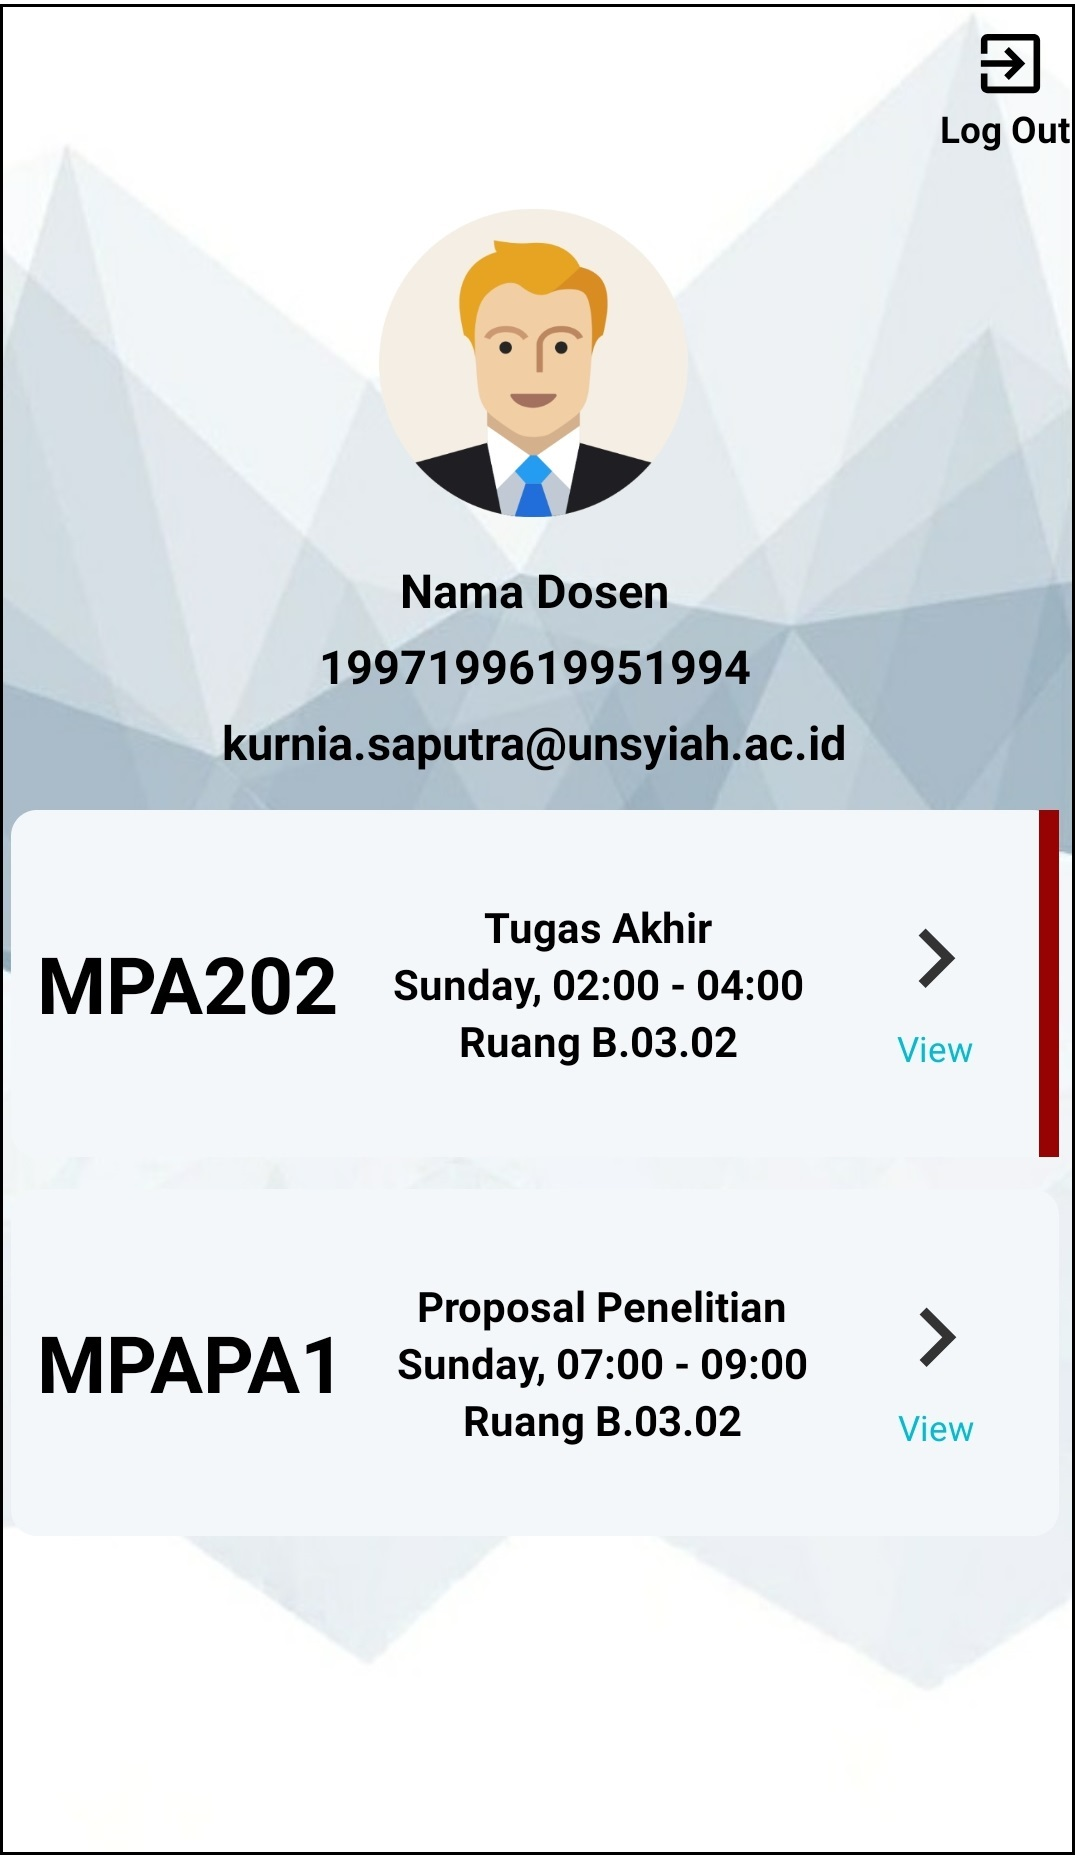
\includegraphics[width=.5\linewidth]{gambar/android/dosen-3}  
  		\caption{Beranda}
	\end{subfigure}
	\begin{subfigure}{.5\textwidth}
  		\centering
  		% include fourth image
  		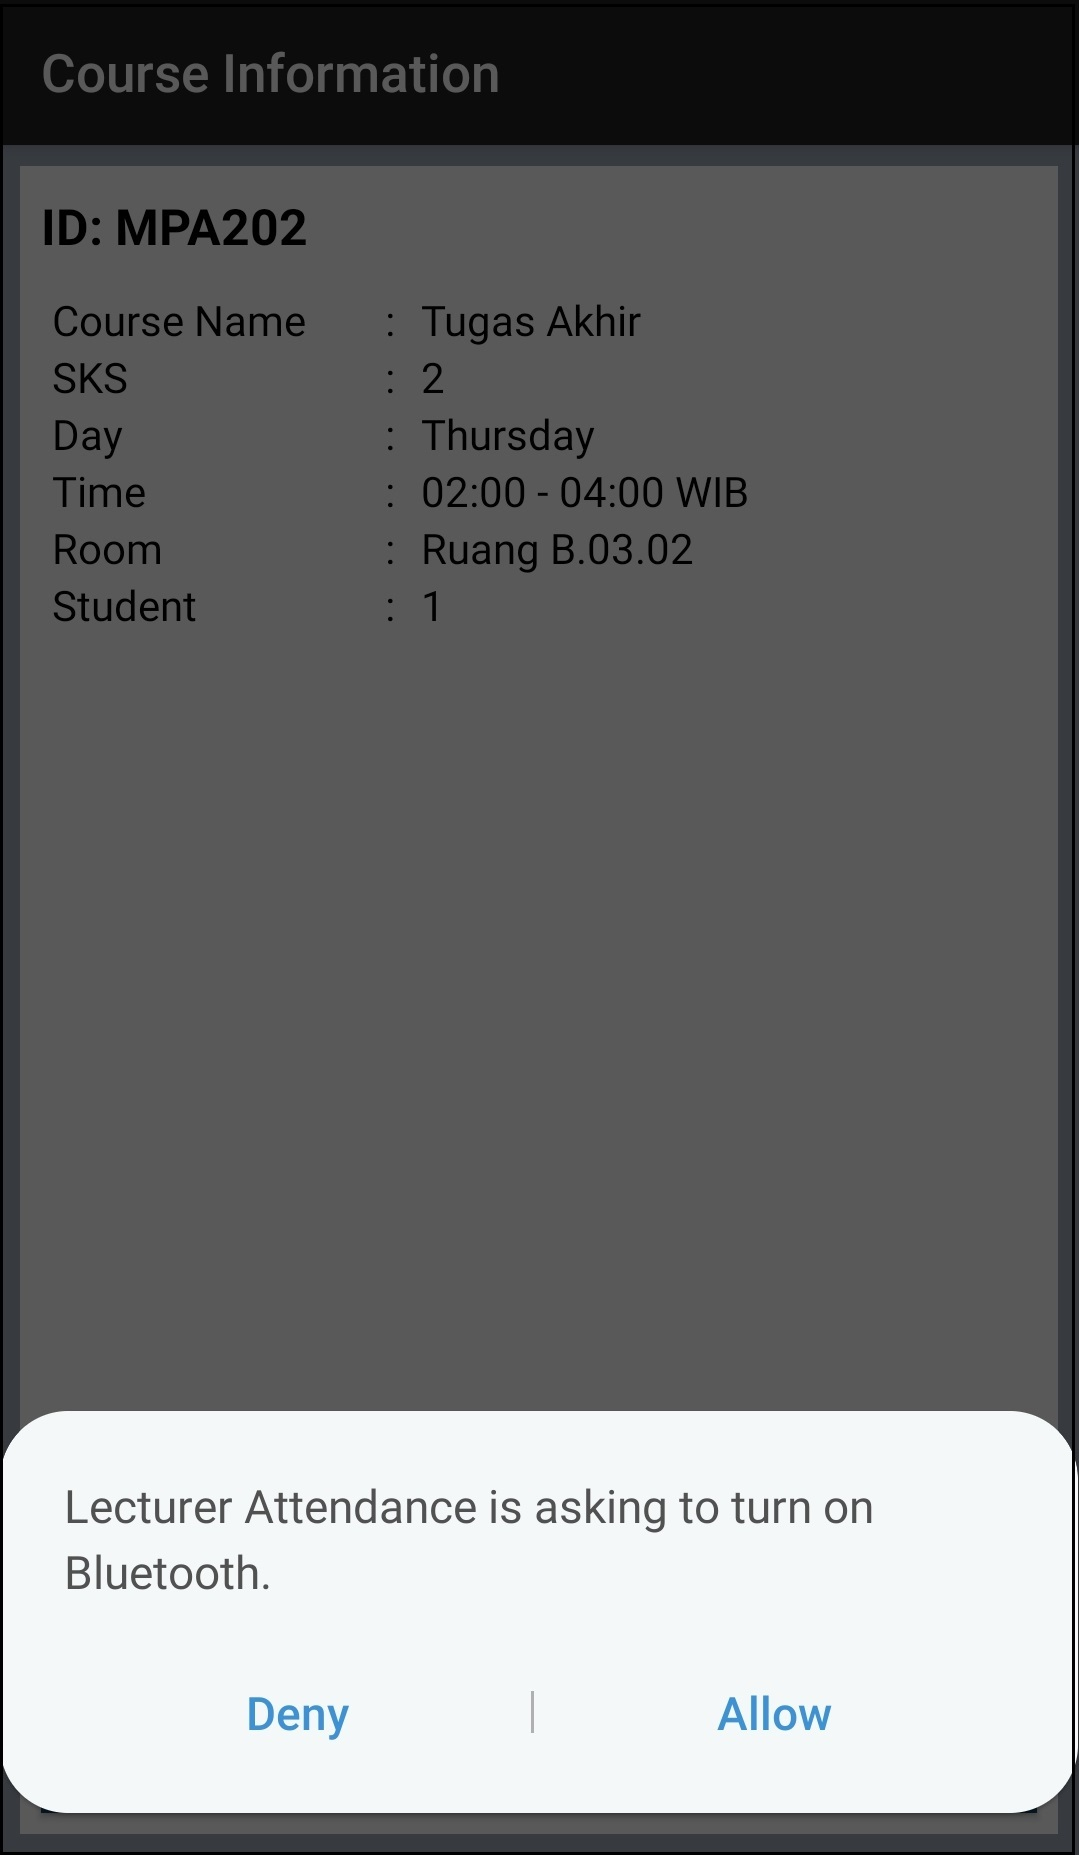
\includegraphics[width=.5\linewidth]{gambar/android/dosen-4}  
  		\caption{Informasi matakuliah}
	\end{subfigure}
		\vspace{0.5cm}
		\caption{Tampilan Halaman Aplikasi Kehadiran Dosen (Bagian 1)}
	\label{aplikasidosenbagian1}
	\end{figure}
	
\vspace{0.5cm}
	\par Gambar \ref{aplikasidosenbagian2} memperlihatkan ketika dosen telah berada di halaman informasi mata kuliah Kemudian, aplikasi akan menampilkan notifikasi untuk menghidupkan Bluetooth apabila Bluetooth pada perangkat belum hidup. Terdapat dua tombol yaitu tombol \textbf{show students} untuk melihat daftar mahasiswa yang mengambil mata kuliah tersebut dan tombol \textbf{start attendance} untuk memulai proses kehadiran. Aplikasi akan melakukan klasifikasi dengan metode K-NN untuk memprediksi lokasi dosen.
	
	\vspace{-0cm}
	\begin{figure} [H]
	\begin{subfigure}{.5\textwidth}
  		\centering
  		% include first image
  		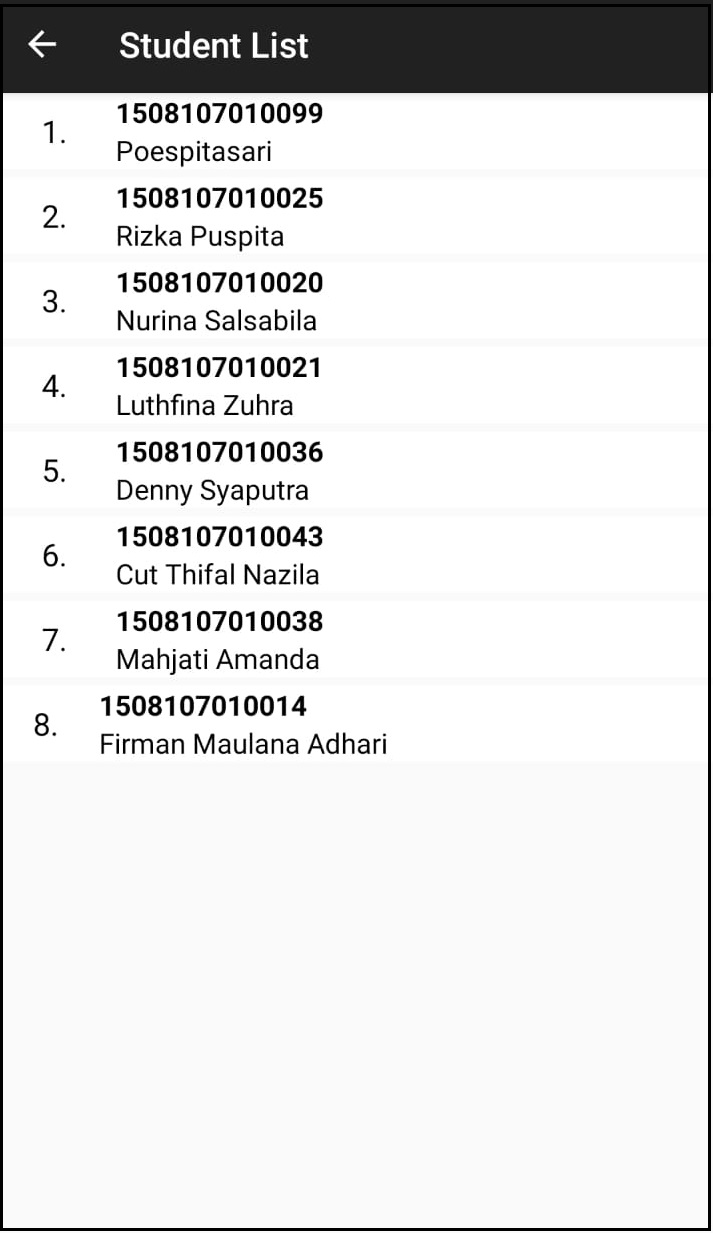
\includegraphics[width=.5\linewidth]{gambar/android/dosen-5}  
  		\caption{Daftar mahasiswa}
	\end{subfigure}
	\begin{subfigure}{.5\textwidth}
  		\centering
  		% include second image
  		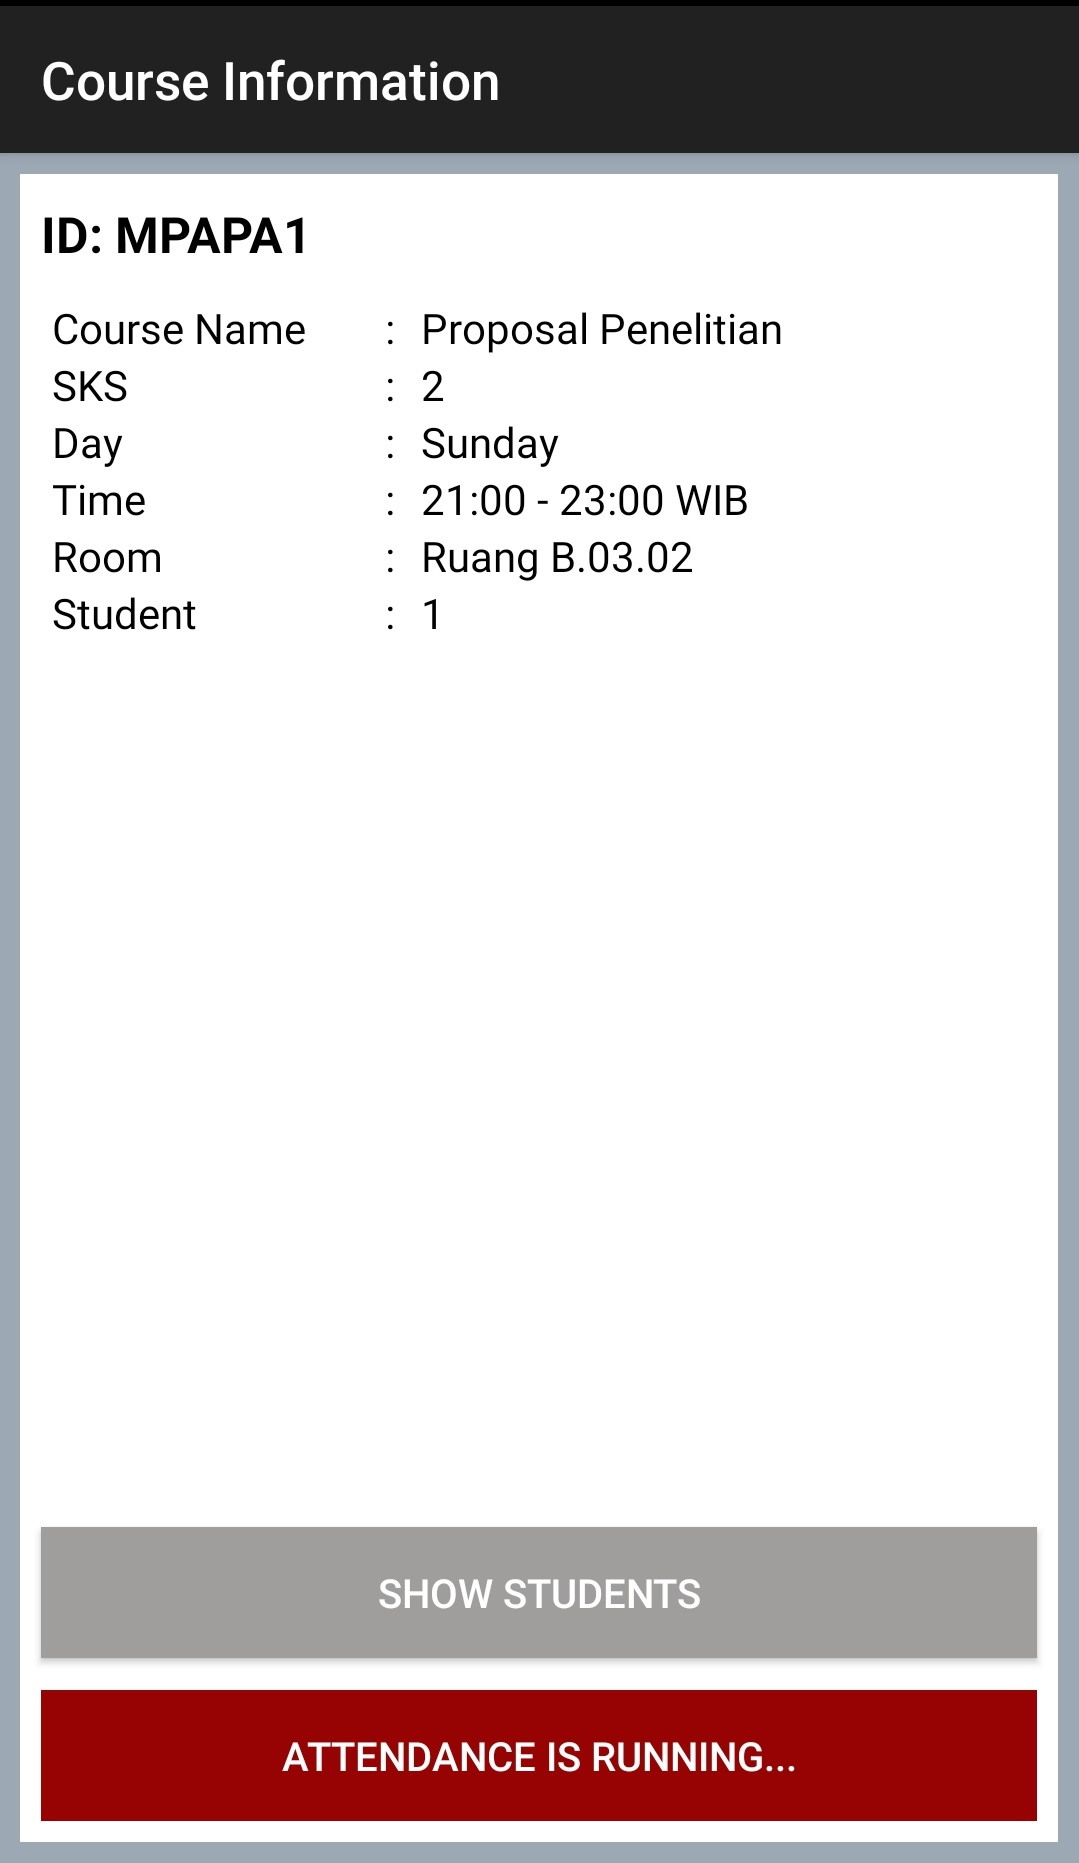
\includegraphics[width=.5\linewidth]{gambar/android/dosen-6}  
  		\caption{Proses kehadiran sedang berjalan}
	\end{subfigure}
	\vspace{1cm}
	\newline
	\begin{subfigure}{.5\textwidth}
  		\centering
  		% include third image
  		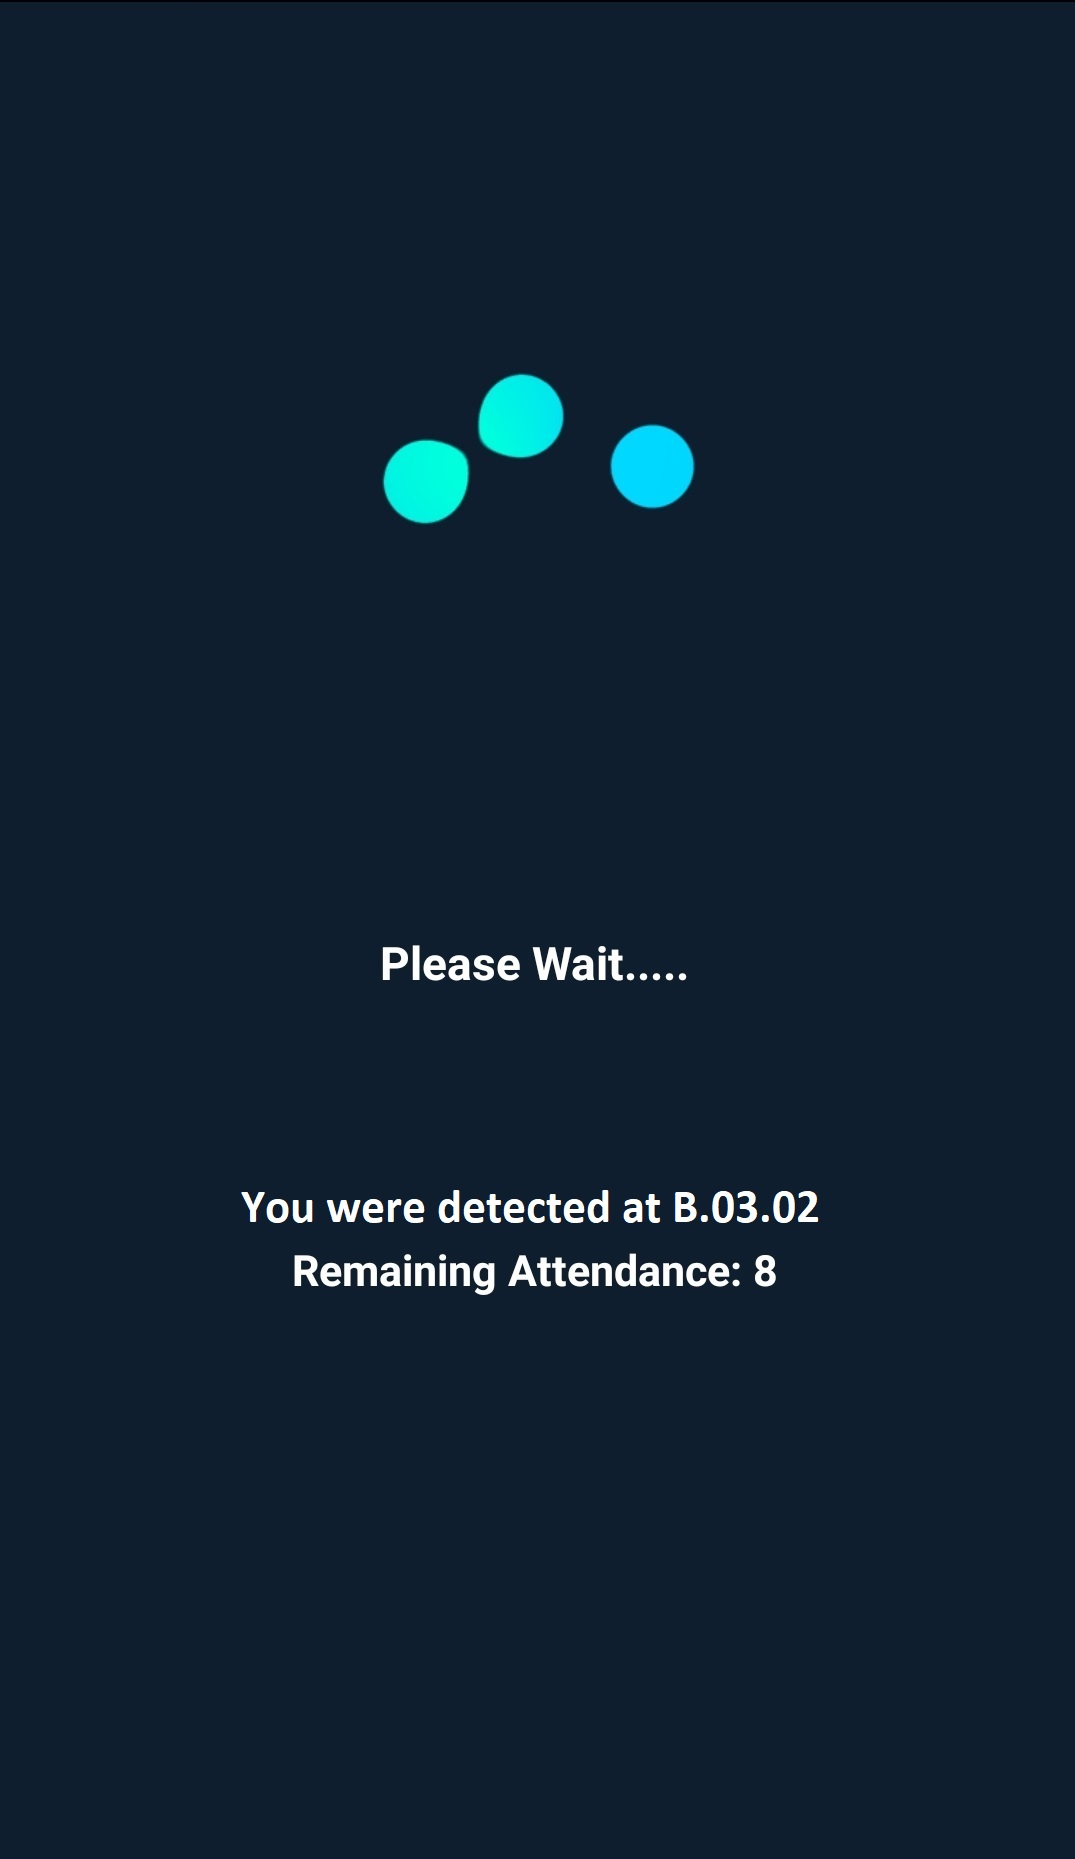
\includegraphics[width=.5\linewidth]{gambar/android/dosen-7}  
  		\caption{Dosen diprediksi di dalam kelas}
	\end{subfigure}
	\begin{subfigure}{.5\textwidth}
  		\centering
  		% include fourth image
  		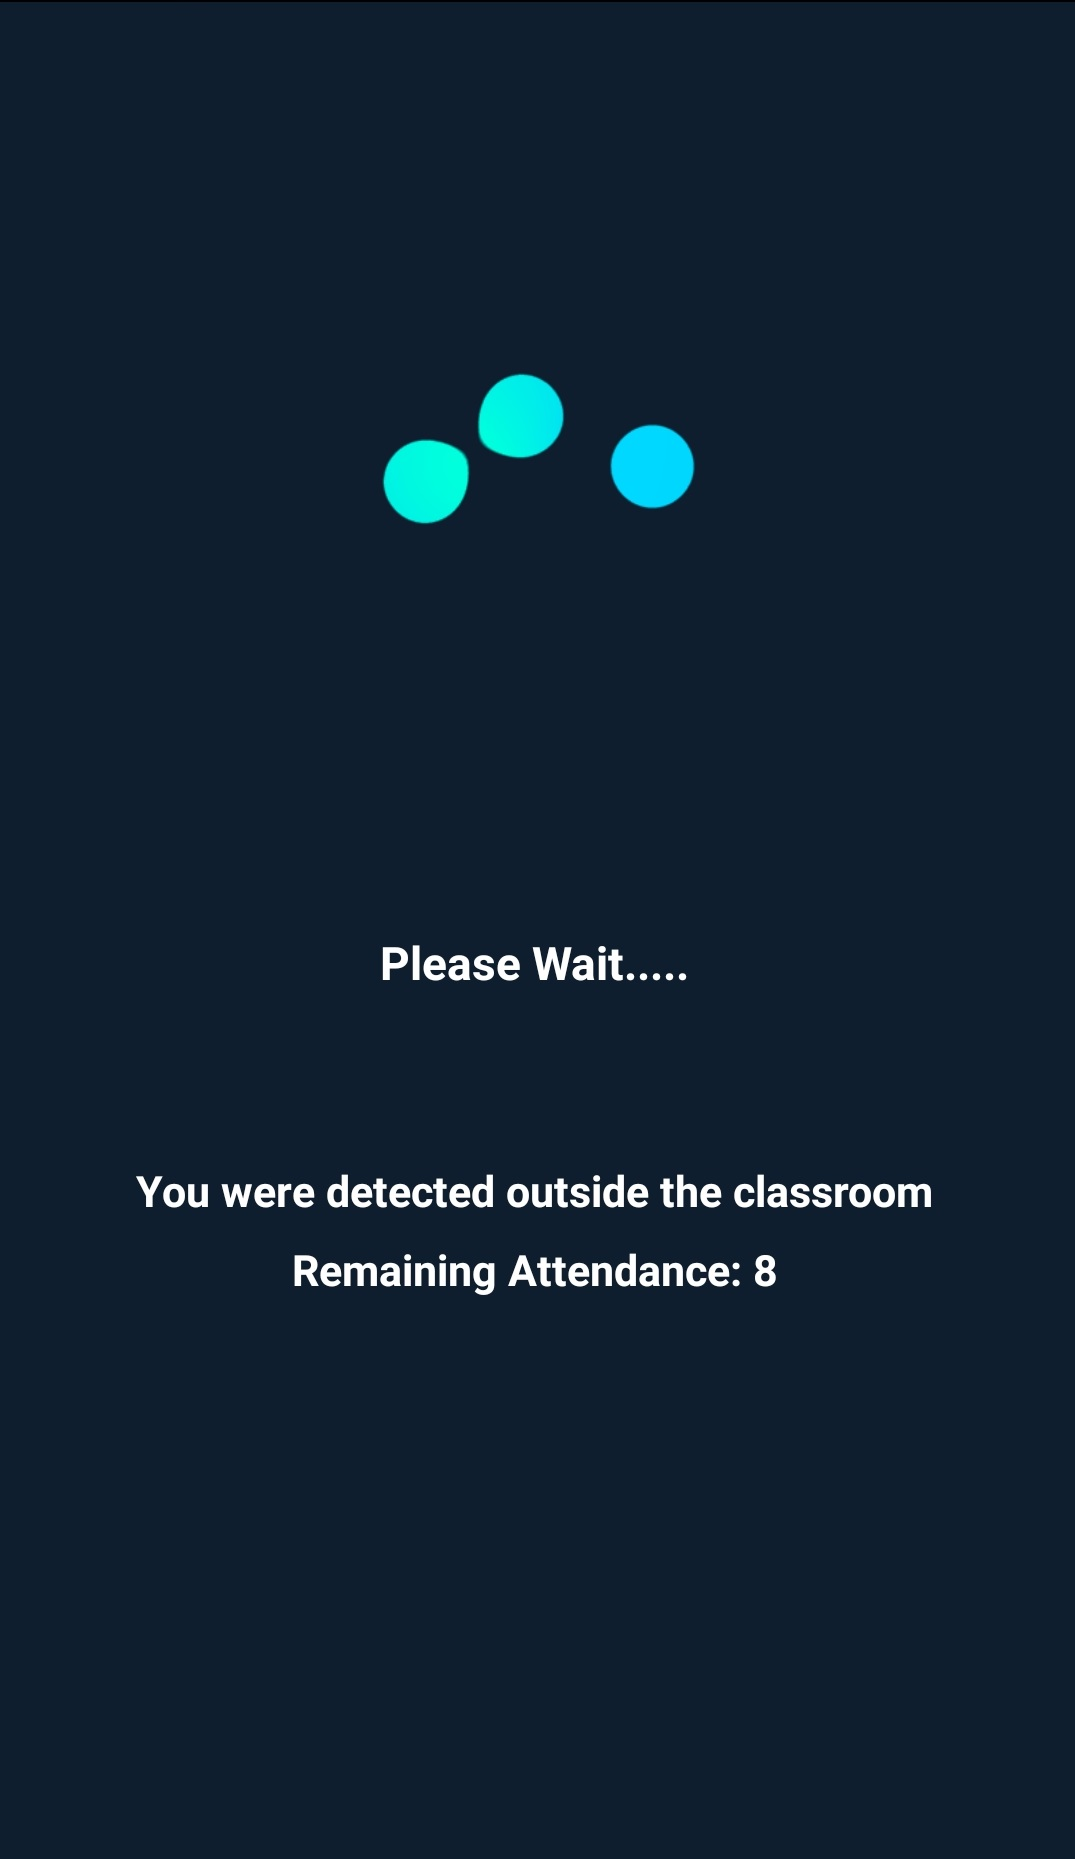
\includegraphics[width=.5\linewidth]{gambar/android/dosen-8}  
  		\caption{Dosen diprediksi di luar kelas}
	\end{subfigure}
		\vspace{0.5cm}
		\caption{Tampilan Halaman Aplikasi Kehadiran Dosen (Bagian 2)}
	\label{aplikasidosenbagian2}
	\end{figure}
	%Akhir Gambar Aplikasi Kehadiran Dosen%
	
	\item Antar Muka Aplikasi Kehadiran Mahasiswa
	
	\par Gambar \ref{aplikasimahasiswabagian1} memperlihatkan ketika mahasiswa belum melakukan \textit{log in}, aplikasi akan menampilkan \textit{landing page} yang berisi langkah-langkah penggunaan aplikasi, lalu mahasiswa akan diarahkan ke halaman \textit{log in}. Untuk melakukan \textit{log in}, mahasiswa diminta untuk memasukkan Nomor Pokok Mahasiswa (NPM) dan kata sandi yang sesuai dengan KRS Online Unsyiah. Setelah itu, mahasiswa akan diarahkan ke halaman beranda apabila telah berhasil melakukan \textit{log in}. Pada halaman beranda, terdapat beberapa menu seperti menu profil, menu daftar mata kuliah dan menu tentang aplikasi, serta informasi mata kuliah hari ini. 
	
	\vspace{-0cm}
	\begin{figure} [H]
	\begin{subfigure}{.5\textwidth}
  		\centering
  		% include first image
  		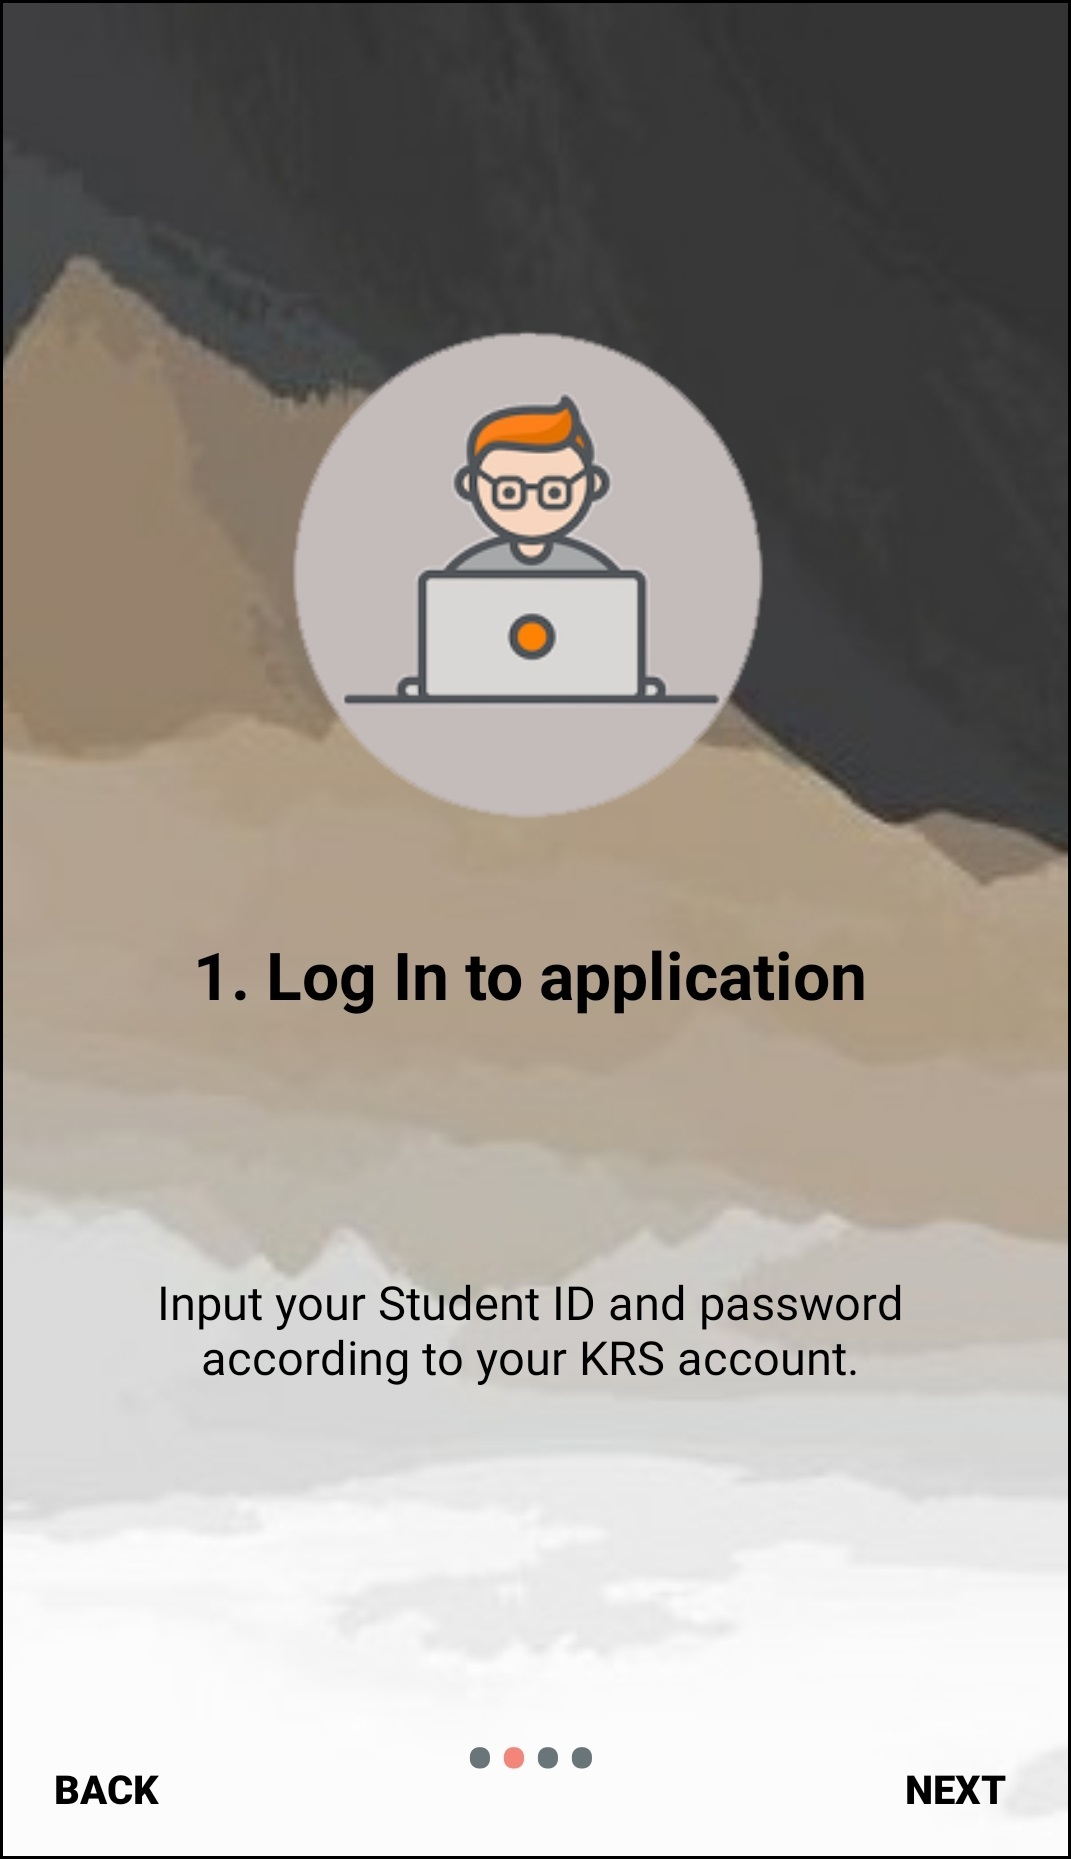
\includegraphics[width=.5\linewidth]{gambar/android/mahasiswa-1}  
  		\caption{\textit{Landing page}}
	\end{subfigure}
	\begin{subfigure}{.5\textwidth}
  		\centering
  		% include second image
  		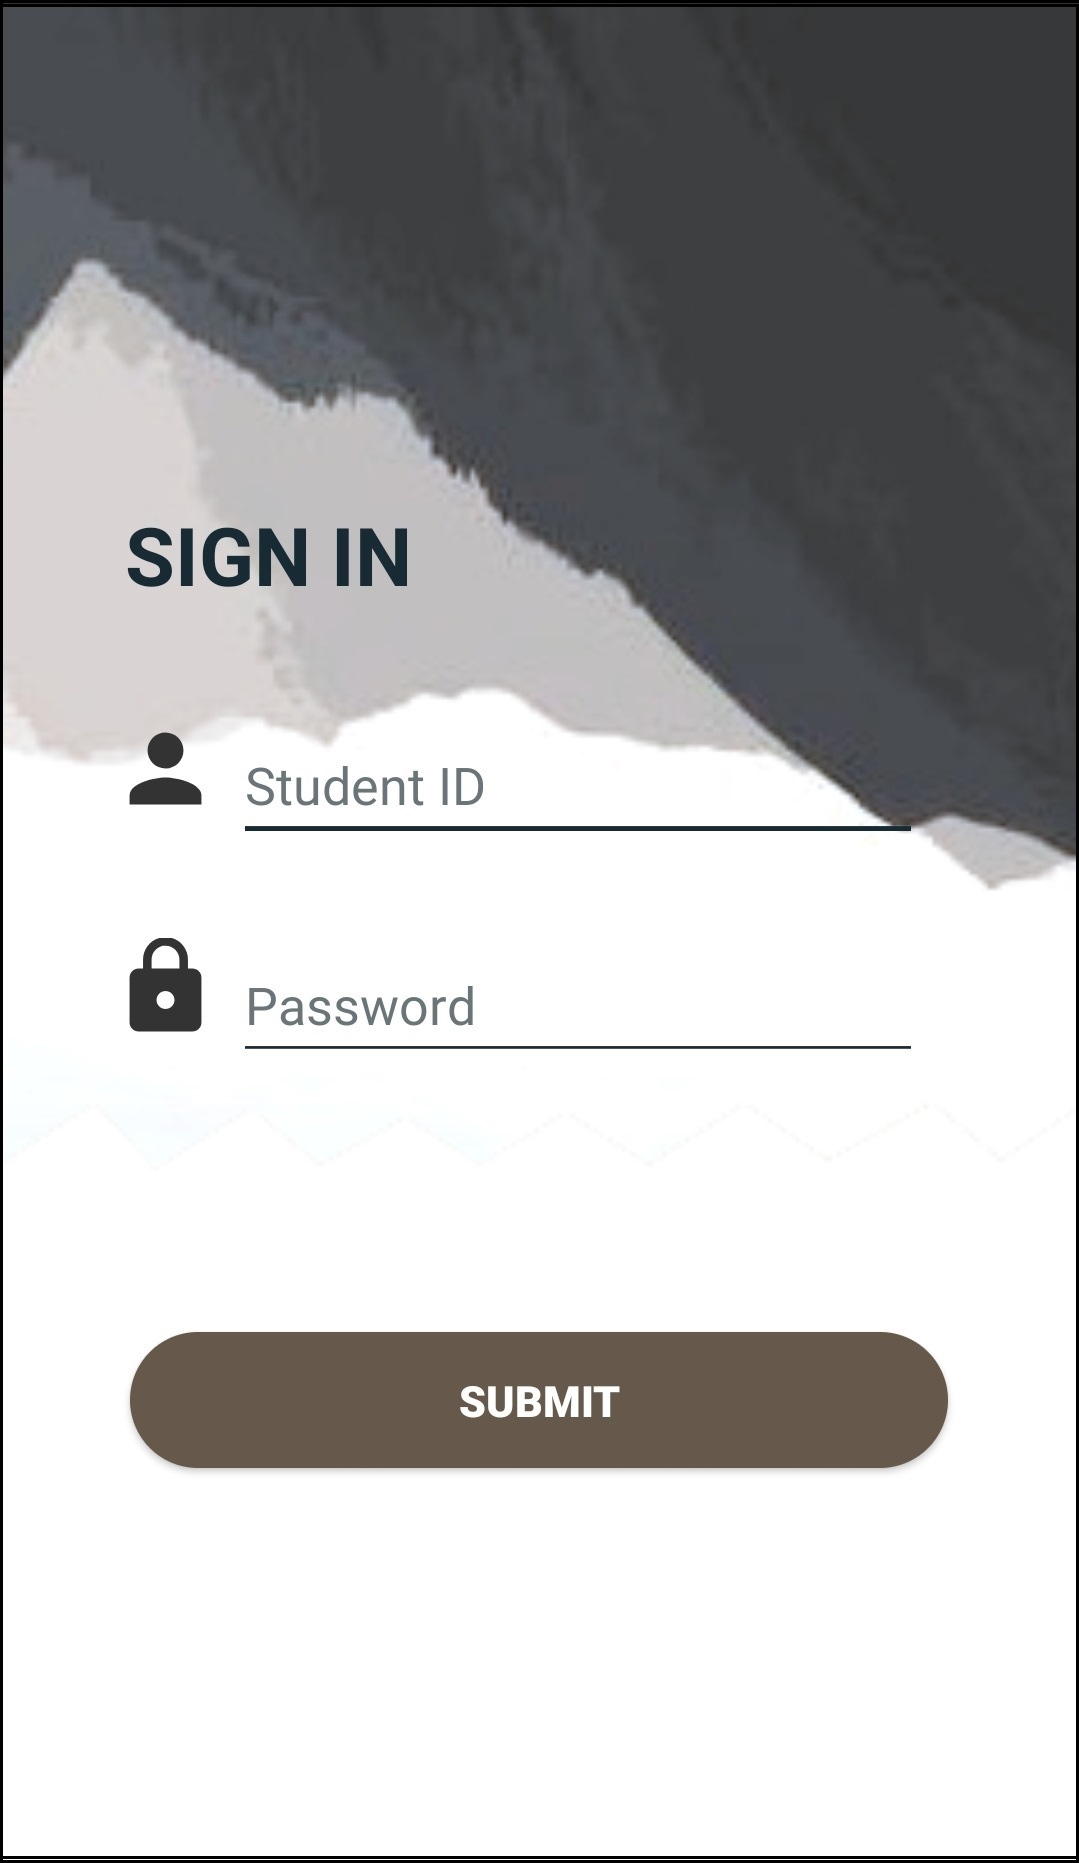
\includegraphics[width=.5\linewidth]{gambar/android/mahasiswa-2}  
  		\caption{\textit{Log in}}
	\end{subfigure}
	\vspace{1cm}
	\newline
	\begin{subfigure}{.5\textwidth}
  		\centering
  		% include third image
  		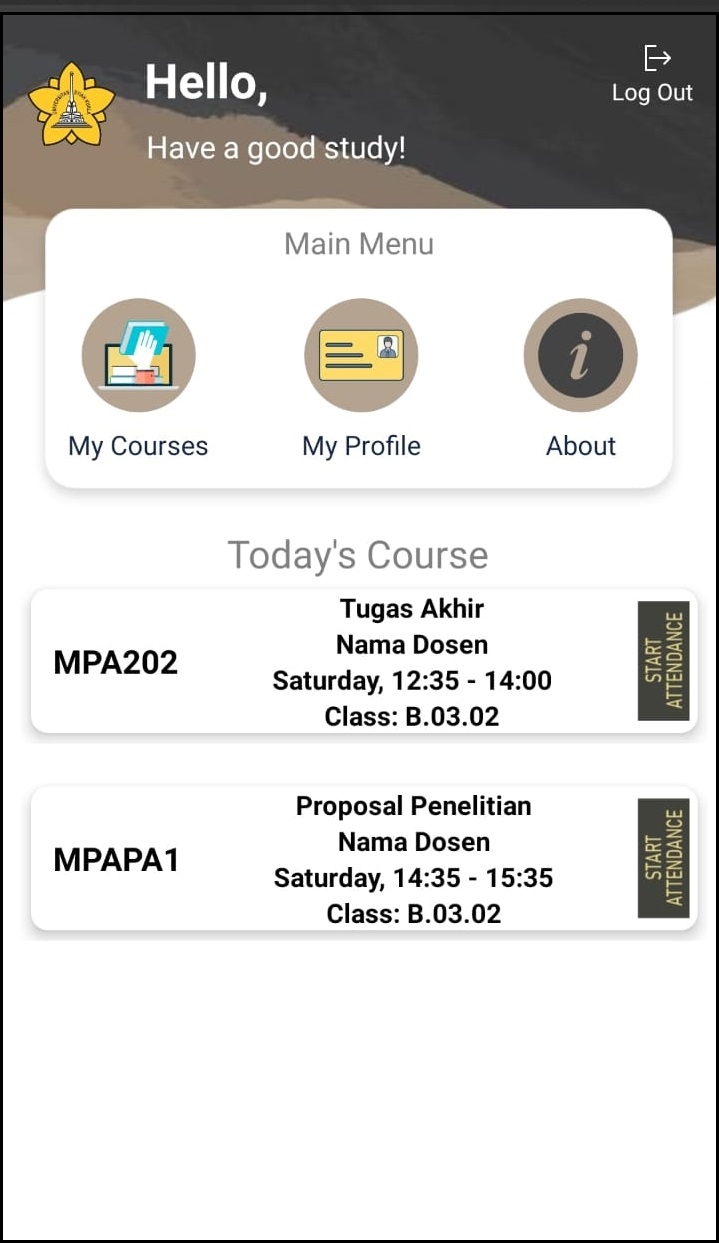
\includegraphics[width=.5\linewidth]{gambar/android/mahasiswa-3}  
  		\caption{Beranda}
	\end{subfigure}
	\begin{subfigure}{.5\textwidth}
  		\centering
  		% include fourth image
  		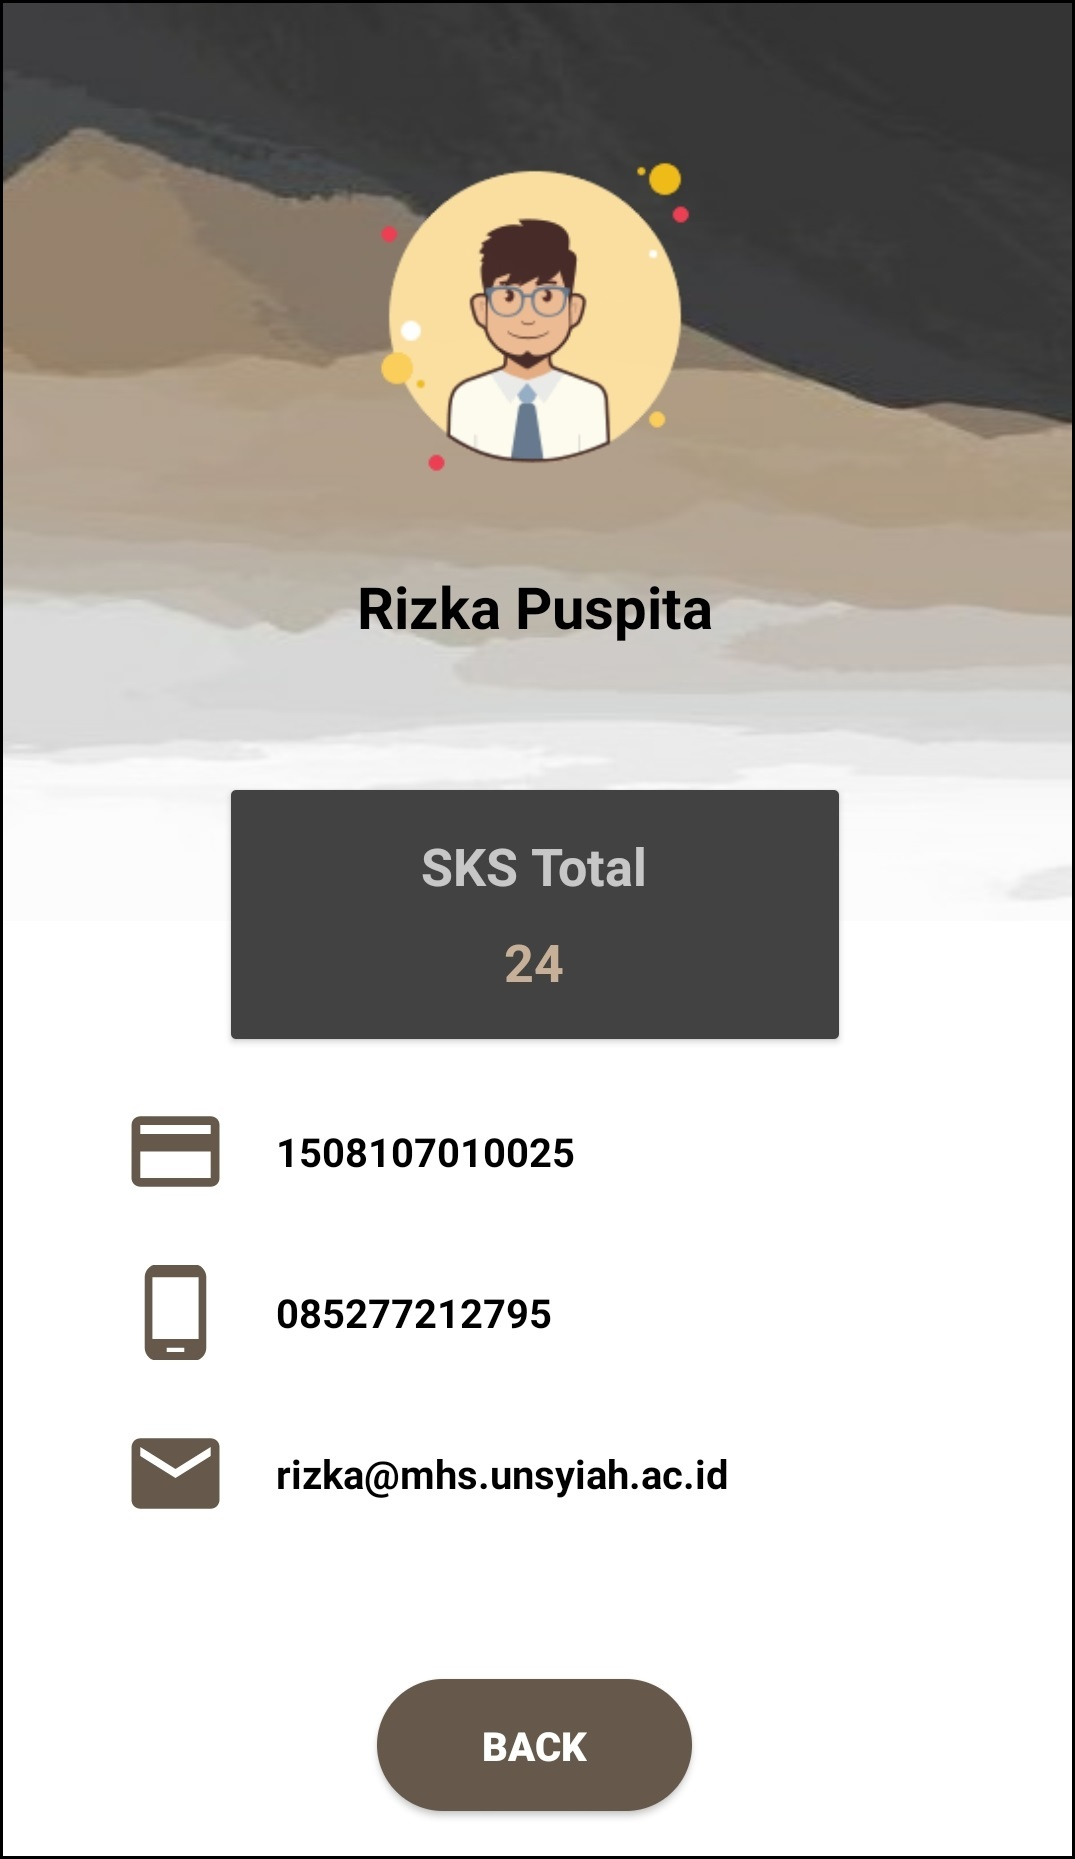
\includegraphics[width=.5\linewidth]{gambar/android/mahasiswa-4}  
  		\caption{Profil}
	\end{subfigure}
		\vspace{0.5cm}
		\caption{Tampilan Halaman Aplikasi Kehadiran Mahasiswa (Bagian 1)}
	\label{aplikasimahasiswabagian1}
	\end{figure}
	
		\par Gambar \ref{aplikasimahasiswabagian1} memperlihatkan daftar mata kuliah yang diambil oleh mahasiswa. Apabila mahasiswa menekan salah satu daftar mata kuliah, aplikasi akan memulai proses kehadiran yang dipicu oleh dosen ketika dosen telah memulai proses kehadiran. Kemudian, aplikasi akan menampilkan notifikasi untuk menghidupkan Bluetooth apabila Bluetooth pada perangkat belum hidup. Jika Bluetooth telah dihidupkan, aplikasi akan melakukan pencatatan kehadiran secara \textit{background proccess} sampai waktu matakuliah berakhir. Aplikasi akan melakukan klasifikasi dengan metode K-NN untuk memprediksi lokasi mahasiswa seperti yang terlihat pada Gambar \ref{aplikasimahasiswabagian2}.
		
	\vspace{-0cm}
	\begin{figure} [H]
	\begin{subfigure}{.5\textwidth}
  		\centering
  		% include first image
  		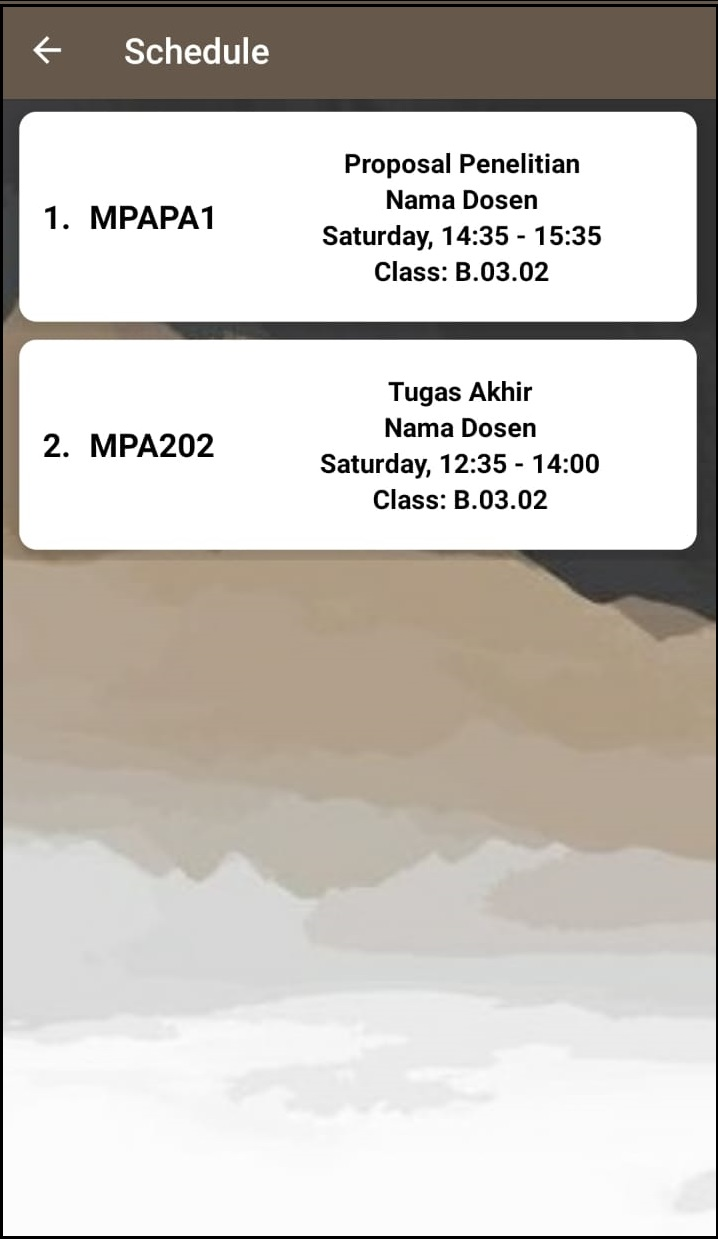
\includegraphics[width=.5\linewidth]{gambar/android/mahasiswa-5}  
  		\caption{Daftar mata kuliah}
	\end{subfigure}
	\begin{subfigure}{.5\textwidth}
  		\centering
  		% include second image
  		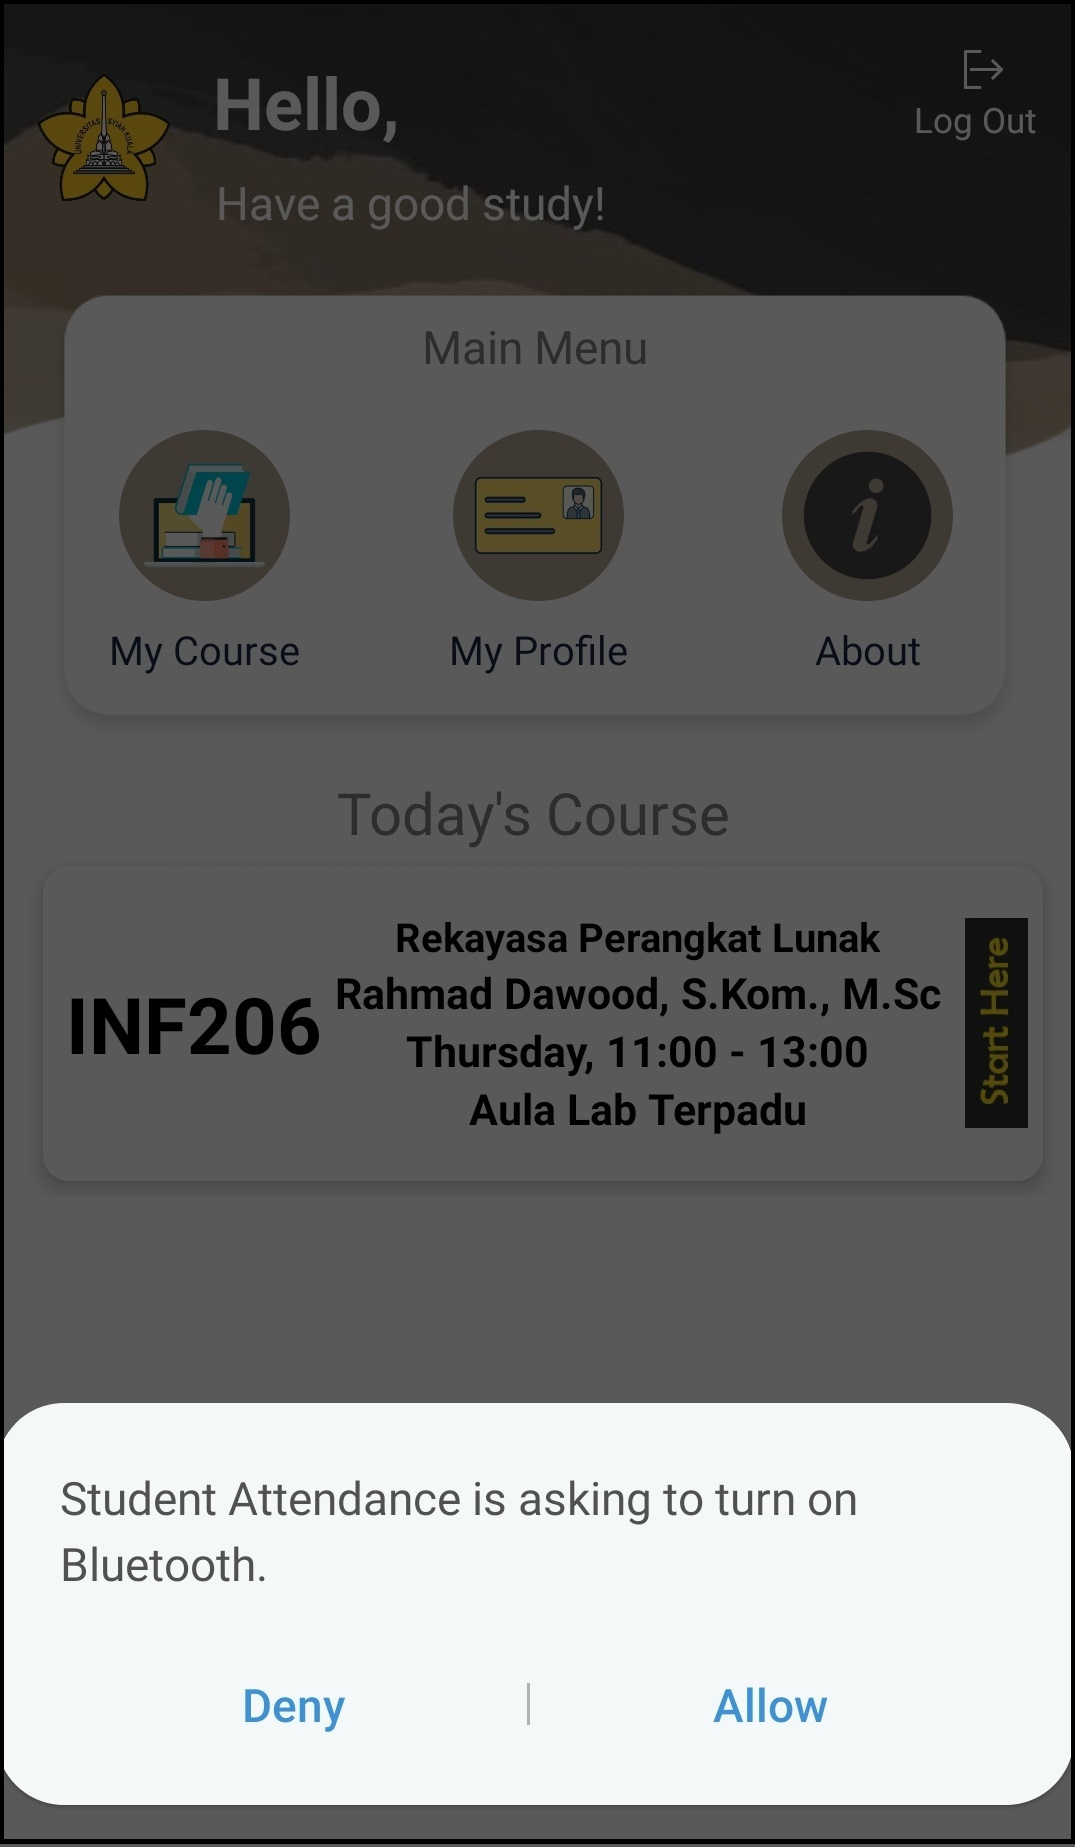
\includegraphics[width=.5\linewidth]{gambar/android/mahasiswa-6}  
  		\caption{Memulai proses kehadiran}
	\end{subfigure}
	\vspace{1cm}
	\newline
	\begin{subfigure}{.5\textwidth}
  		\centering
  		% include third image
  		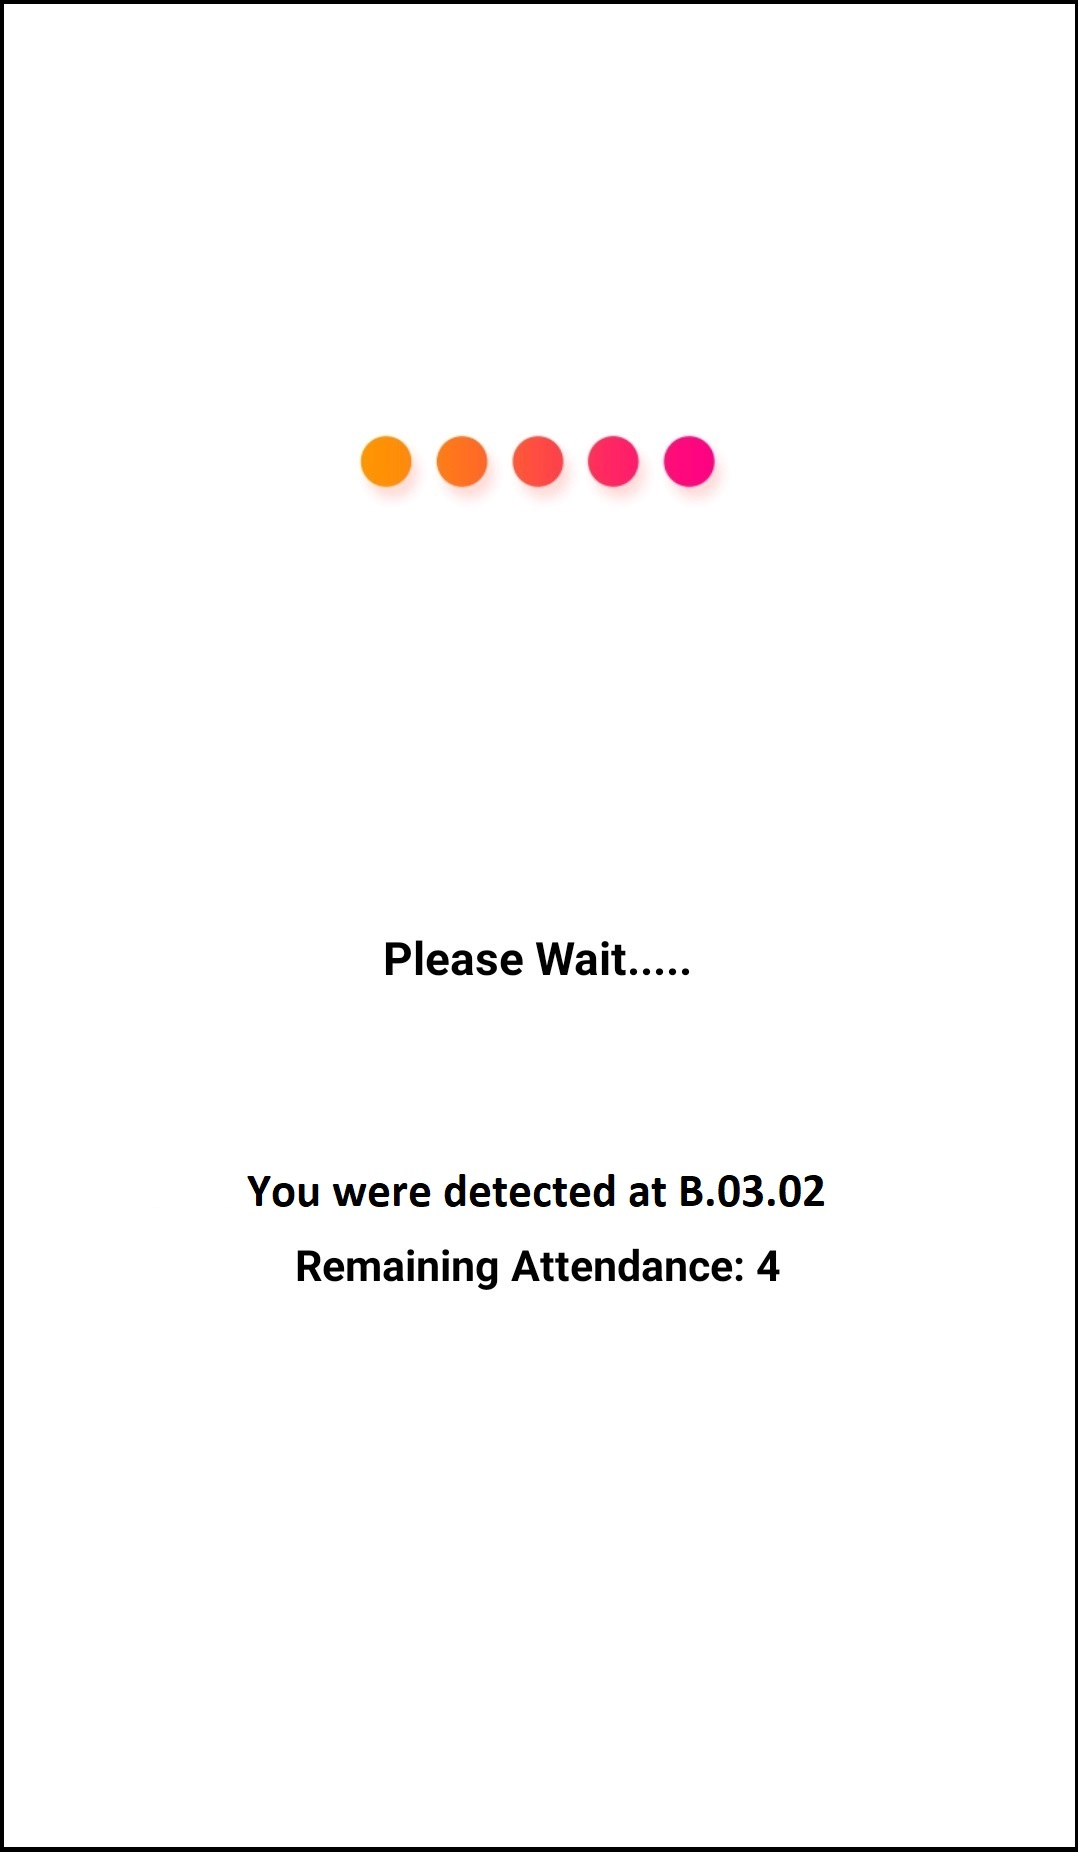
\includegraphics[width=.5\linewidth]{gambar/android/mahasiswa-7}  
  		\caption{Mahasiswa diprediksi di dalam kelas}
	\end{subfigure}
	\begin{subfigure}{.5\textwidth}
  		\centering
  		% include fourth image
  		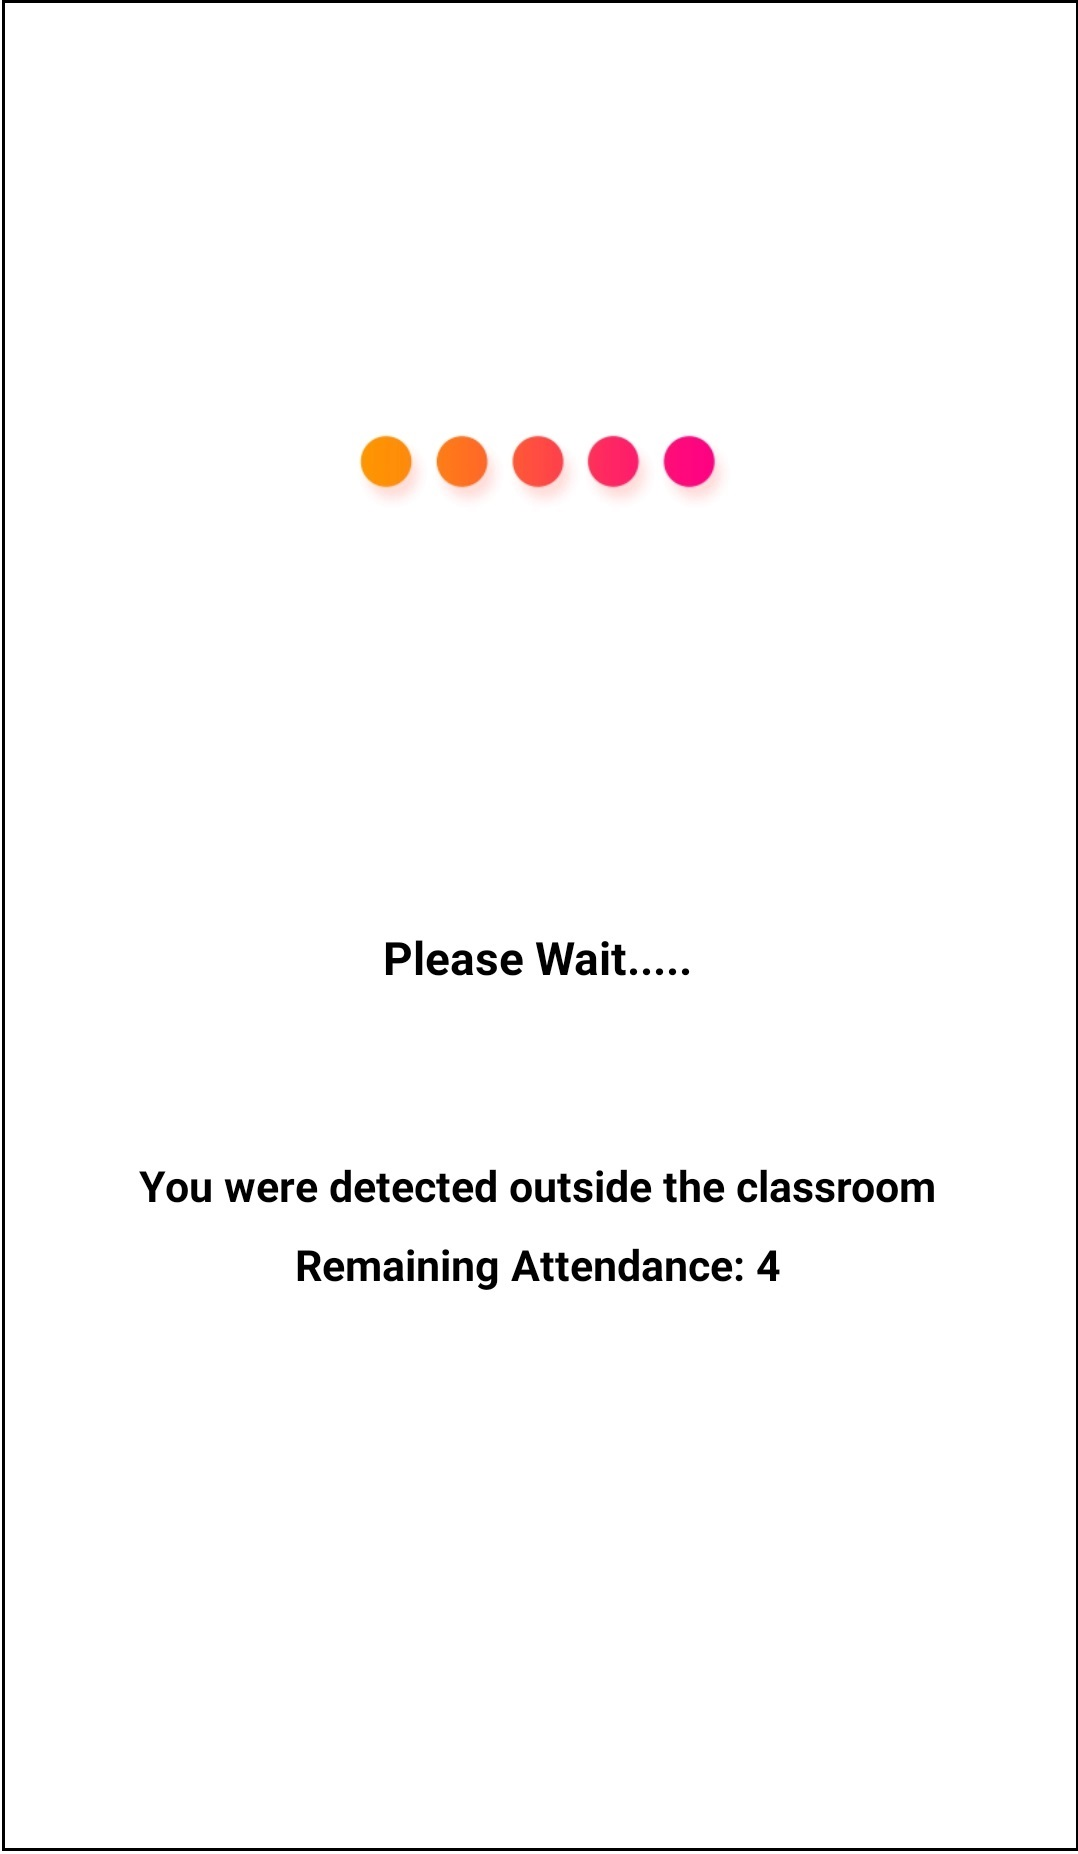
\includegraphics[width=.5\linewidth]{gambar/android/mahasiswa-8}  
  		\caption{Mahasiswa diprediksi di luar kelas}
	\end{subfigure}
		\vspace{0.5cm}
		\caption{Tampilan Halaman Aplikasi Kehadiran Mahasiswa (Bagian 2)}
	\label{aplikasimahasiswabagian2}
	\end{figure}

	%Akhir Gambar Aplikasi Kehadiran Mahasiswa%
	
		\end{enumerate}
		
%%%%%%%%%%%%%%%%%%%%%%%%%%%%%%%%%%%%%%%%%%%akhir perancangan aplikasi mapping%%%%%%%%%%%%%%%%%%%%%%%%%%%%%%%%%%%%%%%%%%%%%%%%%%%
	\subsection{Pembuatan Sistem}
	
	\begin{enumerate}[a.]
		\item Aplikasi Mapping
		\\ Aplikasi \textit{mobile} berbasis Android yang dikembangkan menggunakan bahasa pemrograman Java dengan bantuan IDE Android Studio. Media penyimpanan basis data pada aplikasi ini menggunakan SQLite. SQLite merupakan media penyimpanan lokal untuk setiap aplikasi yang sudah terpasang di perangkat Android, dikarenakan aplikasi ini hanya perlu menyimpan data-data hasil pemindaian kekuatan sinyal Bluetooth. Aplikasi mapping ini juga sudah memiliki sertifikat Hak Kekayaan Intelektual (HKI) dengan nomor EC00201972853 yang dapat dilihat pada lampiran 1. Potongan kode program untuk melakukan pemindaian kekuatan sinyal Bluetooth dapat dilihat pada Program 4.1 berikut ini.
		\vspace{0.4cm}
			\lstset{language=Java,
			basicstyle=\ttfamily\scriptsize\color{black},
			keywordstyle=\color{javapurple}\bfseries,
			stringstyle=\color{javared},
			commentstyle=\color{javagreen},
			morecomment=[s][\color{javadocblue}]{/**}{*/},
			numbers=left,
			numberstyle=\tiny\color{black},
			showstringspaces=false,
			numbersep=10pt,
			tabsize=4,
			showspaces=false,
			showstringspaces=false,
			autogobble=true,
			xleftmargin=2em
		}
	\begin{lstlisting}[label=programScanBle]
    private HashMap<String, BTLEDevice> mBTDevicesHashMap;
    private Ble pojoBle;

    mBTDevicesHashMap = new HashMap<>(); // membuat objek kelas HashMap.
	
	/**
     * @param device parameter dari kelas BluetoothDevice yang akan ditambahkan.
     * @param rssi rssi dari kelas BluetoothDevice.
     */
    public void addDevice(BluetoothDevice device, int rssi) {
     String address = device.getAddress();
      if (!mBTDevicesHashMap.containsKey(address)) {
         if (address.equals(pojoBle.ADDRESS_1) || address.equals(pojoBle.ADDRESS_2) 
             .... 
             || address.equals(pojoBle.ADDRESS_9));
         {
             BTLEDevice btleDevice = new BTLEDevice(device);
             btleDevice.setRSSI(rssi);
             mBTDevicesHashMap.put(address, btleDevice);
             mBTDevicesArrayList.add(btleDevice);
         }
      }
      else {
            mBTDevicesHashMap.get(address).setRSSI(rssi);
        }
    }
	\end{lstlisting}
	 \captionof{lstlisting}{Potongan Kode Program Membaca Informasi Bluetooth.}

		
		\item Aplikasi Kehadiran Dosen
		\\ Aplikasi \textit{mobile} berbasis Android yang dikembangkan menggunakan bahasa pemrograman Java dengan bantuan IDE Android Studio. Media penyimpanan aplikasi ini menggunakan basis data server yaitu MySQL. Basis data server tersebut diakses melalui REST server API yang dibangun menggunakan bahasa pemrograman PHP. Aplikasi ini bertindak sebagai klien. Oleh karena itu, aplikasi ini menggunakan \textit{library} Retrofit untuk melakukan \textit{request} ke server dan menghandle \textit{response} dalam bentuk JavaScript Object Notation (JSON). Proses pengiriman data dari klien ke server dilakukan ketika dosen menekan tombol \textbf{start attendance} pada aplikasi. %Potongan kode program yang dibuat untuk melakukan pengiriman data dapat dilihat pada kode \ref{programStartAbsen} berikut ini. 
		Seorang dosen dapat terhitung menghadiri perkuliahan pada aplikasi apabila syarat-syarat di bawah ini terpenuhi:
		\begin{enumerate}[1.]
		\item Dosen menekan tombol \textbf{start attendance} 50 menit sebelum mata kuliah berakhir. 
		\item Dosen menekan tombol \textbf{start attendance} sesuai waktu yang telah ditentukan. Penentuan lokasi dilakukan dengan menggunakan metode klasifikasi K-NN yang dapat dilihat pada Program 4.2 berikut ini.
		\vspace{0.4cm}
		% KODE KNN%
	\begin{lstlisting}[label=programKNNDosen]
	public void stopScan() {
    // ambil semua nilai yang ada di HashMap (Bluetooth yang terdeteksi).
     Set<String> keys = mBTDevicesHashMap.keySet();
     String empty = "";
     String sinyal = "";
     for(String key : keys ) {
         empty += mBTDevicesHashMap.get(key).getAddress()+"\n";
         sinyal += mBTDevicesHashMap.get(key).getRSSI()+"\n";
     }
     //inisialisasi lokasi file data training.
     String train = "data_training_sequence_point.csv";
     //untuk mengambil data hasil pemindaian yg tersimpan di Hash.
     BTLE_Device ble1 = mBTDevicesHashMap.get(Ble.ADDRESS_1);
     ....  
     BTLE_Device ble9 = mBTDevicesHashMap.get(Ble.ADDRESS_9);
     //untuk kasih nilai default apabila sinyal Bluetooth tidak dapat.
     int rssi1 = ble1 == null ? -110 : ble1.getRSSI();
     ....
     int rssi9 = ble9 == null ? -110 : ble9.getRSSI();
     double[] testData = {rssi1, rssi2, ..., rssi9};
      try {
          InputStream streamTrain = getAssets().open(train);
          label = (int) KNN.knn(streamTrain, testData, 5);
          boolean masukKelas = (label == idRuang);
      } catch (IOException e) {
          e.printStackTrace();
       	}
    }
    
    \end{lstlisting}
    \captionof{lstlisting}{Potongan Kode Program Klasifikasi Metode K-NN Aplikasi Kehadiran Dosen.}

		\item Setiap mata kuliah memiliki satu sesi proses pencatatan kehadiran setiap 10 menit. Di setiap sesi tersebut, setiap aplikasi kehadiran dosen akan melakukan pencatatan kehadiran dengan pada waktu acak antara menit pertama hingga menit ke-10 setiap sesi. Sebagai contoh, mata kuliah A dimulai pada pukul 14:00 sampai pukul 16:00. Apabila satu sesi dilakukan per-10 menit sekali, maka total sesinya adalah 12 kali untuk proses pencatatan kehadiran. Misalnya sesi pertama dimulai pada pukul 14:02, pada saat itu aplikasi akan memprediksi lokasi dosen dan mengirimnya ke server untuk disesuaikan apakah kelas yang diprediksi saat itu sama dengan kelas sebenarnya. Jika prediksinya sesuai, maka dosen tersebut terhitung hadir. Kemudian, sesi kedua dimulai pada pukul 14:18. Jika prediksi yang dilakukan tidak sesuai, maka dosen tersebut terhitung tidak hadir. Proses tersebut akan berlangsung sampai sesi terakhir. Dari hasil prediksi setiap sesi tersebut, akan dihitung \textit{threshold} minimal 80\% dari jumlah proses pencatatan kehadiran yang dilakukan oleh aplikasi. 
		\end{enumerate}
		
		\vspace{0.5cm}
		\item Aplikasi Kehadiran Mahasiswa
		\\ Aplikasi \textit{mobile} berbasis Android yang dikembangkan menggunakan bahasa pemrograman Java dengan bantuan IDE Android Studio. Media penyimpanan aplikasi ini menggunakan basis data server yaitu MySQL. Basis data server tersebut diakses melalui REST server API yang dibangun menggunakan bahasa pemrograman PHP. Aplikasi ini bertindak sebagai klien. Oleh karena itu, aplikasi ini menggunakan \textit{library} Retrofit untuk melakukan \textit{request} ke server dan menghandle \textit{response} dalam bentuk JavaScript Object Notation (JSON). Proses pengiriman data dari klien ke server dilakukan ketika mahasiswa menekan tombol \textbf{start attendance} pada aplikasi. 
\newline
Seorang mahasiswa dapat terhitung menghadiri perkuliahan pada aplikasi apabila syarat-syarat di bawah ini terpenuhi:
		\begin{enumerate}[1.]
		\item Mahasiswa menekan tombol \textbf{start attendance} ketika perkuliahan sudah dimulai oleh dosen. Penentuan lokasi dilakukan dengan menggunakan metode klasifikasi K-NN yang dapat dilihat pada Program 4.3 berikut ini.
		\vspace{0.4cm}
		% KODE KNN%
	\begin{lstlisting}[label=programKNNMahasiswa]
	public void stopScan() {
    // ambil semua nilai yang ada di HashMap (Bluetooth yang terdeteksi).
     Set<String> keys = mBTDevicesHashMap.keySet();
     String empty = "";
     String sinyal = "";
     for(String key : keys ) {
         empty += mBTDevicesHashMap.get(key).getAddress()+"\n";
         sinyal += mBTDevicesHashMap.get(key).getRSSI()+"\n";
     }
     //inisialisasi lokasi file data training.
     String train = "data_training_sequence_point.csv";
     //untuk mengambil data hasil pemindaian yg tersimpan di Hash.
     BTLE_Device ble1 = mBTDevicesHashMap.get(Ble.ADDRESS_1);
     ....  
     BTLE_Device ble9 = mBTDevicesHashMap.get(Ble.ADDRESS_9);
     //untuk kasih nilai default apabila sinyal Bluetooth tidak dapat.
     int rssi1 = ble1 == null ? -110 : ble1.getRSSI();
     ....
     int rssi9 = ble9 == null ? -110 : ble9.getRSSI();
     double[] testData = {rssi1, rssi2, ..., rssi9};
      try {
          InputStream streamTrain = getAssets().open(train);
          label = (int) KNN.knn(streamTrain, testData, 5);
          boolean masukKelas = (label == idRuang);
      } catch (IOException e) {
          e.printStackTrace();
       	}
    }
    \end{lstlisting}
    \captionof{lstlisting}{Potongan Kode Program Klasifikasi Metode K-NN Aplikasi Kehadiran Mahasiswa.}
    
		\vspace{2cm}
		\item Setiap mata kuliah memiliki satu sesi proses pencatatan kehadiran setiap 10 menit. Di setiap sesi tersebut, setiap aplikasi kehadiran mahasiswa akan melakukan pencatatan kehadiran dengan pada waktu acak antara menit pertama hingga menit ke-10 setiap sesi. Sebagai contoh, mata kuliah B dimulai pada pukul 08:30 sampai pukul 10:30. Apabila satu sesi dilakukan per-10 menit sekali, maka total sesinya adalah 12 kali untuk proses pencatatan kehadiran. Misalnya sesi pertama dimulai pada pukul 08:37, pada saat itu aplikasi akan memprediksi lokasi mahasiswa dan mengirimnya ke server untuk disesuaikan apakah kelas yang diprediksi saat itu sama dengan kelas sebenarnya. Jika prediksinya sesuai, maka mahasiswa tersebut terhitung hadir. Kemudian, sesi kedua dimulai pada pukul 08:49. Jika prediksi yang dilakukan tidak sesuai, maka mahasiswa tersebut terhitung tidak hadir. Proses tersebut akan berlangsung sampai sesi terakhir. Dari hasil prediksi setiap sesi tersebut, akan dihitung \textit{threshold} minimal 80\% dari jumlah proses pencatatan kehadiran yang dilakukan oleh aplikasi.
		\end{enumerate}

	\item Aplikasi Rekap Kehadiran Dosen dan Mahasiswa Berbasis Web
	\\
	Aplikasi berbasis web ini dikembangkan dengan menggunakan bahasa pemrograman PHP dengan menggunakan prinsip MVC (Model-View-Controller). Dimana \textit{model} sebagai struktur data dan basis datanya, \textit{view} untuk menampilkan isi halaman web yang dibangun dan \textit{controller} merupakan alur bisnis sebagai jembatan \textit{model} dan \textit{view} yang menanggapi HTTP \textit{request} yang datang dari pengguna melalui \textit{browser}. Tampilan halaman \textit{log in} pada aplikasi ini dapat dilihat pada Gambar \ref{web-login}, tampilan halaman daftar kehadiran dosen dapat dilihat pada Gambar \ref{web-daftar-dosen}, tampilan halaman daftar kehadiran mahasiswa dapat dilihat pada Gambar \ref{web-daftar-mahasiswa}. Fitur utama pada aplikasi ini adalah dapat mengunduh daftar kehadiran dosen dan mahasiswa dengan format CSV untuk keperluan merekap data yang dapat dilihat pada Gambar \ref{web-csv-dosen} dan Gambar \ref{web-csv-mahasiswa}.  
	\vspace{-0.2cm}
		\begin{figure}[H]
		\center
		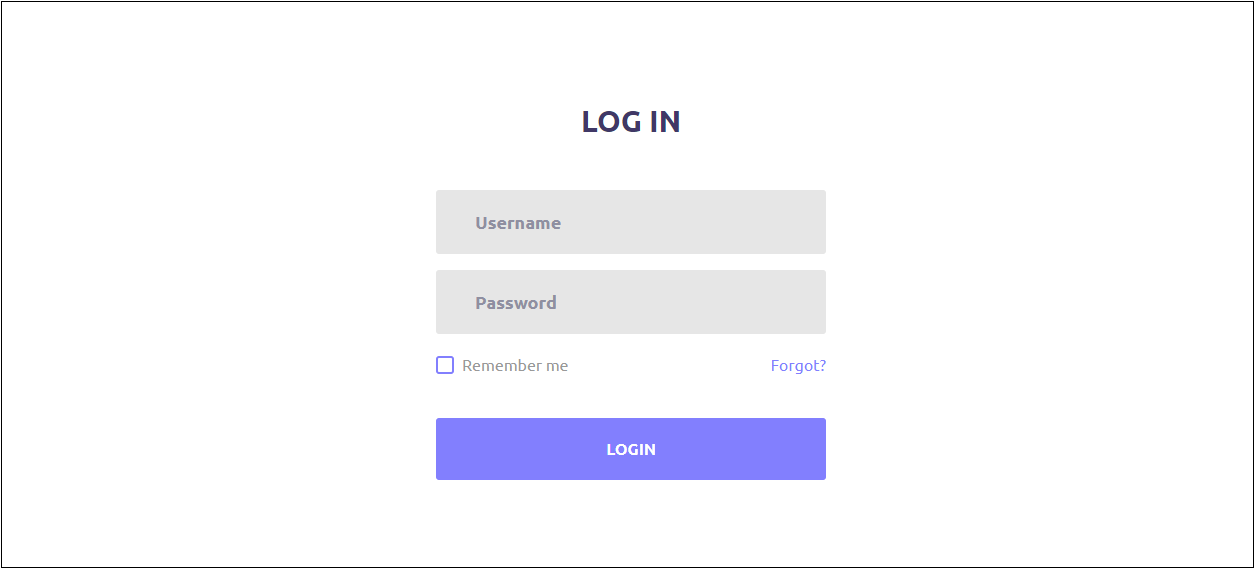
\includegraphics [width = 13cm, height= 6cm]{gambar/web/login}
		\caption{Halaman \textit{Log In}}
		\label{web-login}
		\end{figure}
		
		\vspace{-0.2cm}
		\begin{figure}[H]
		\center
		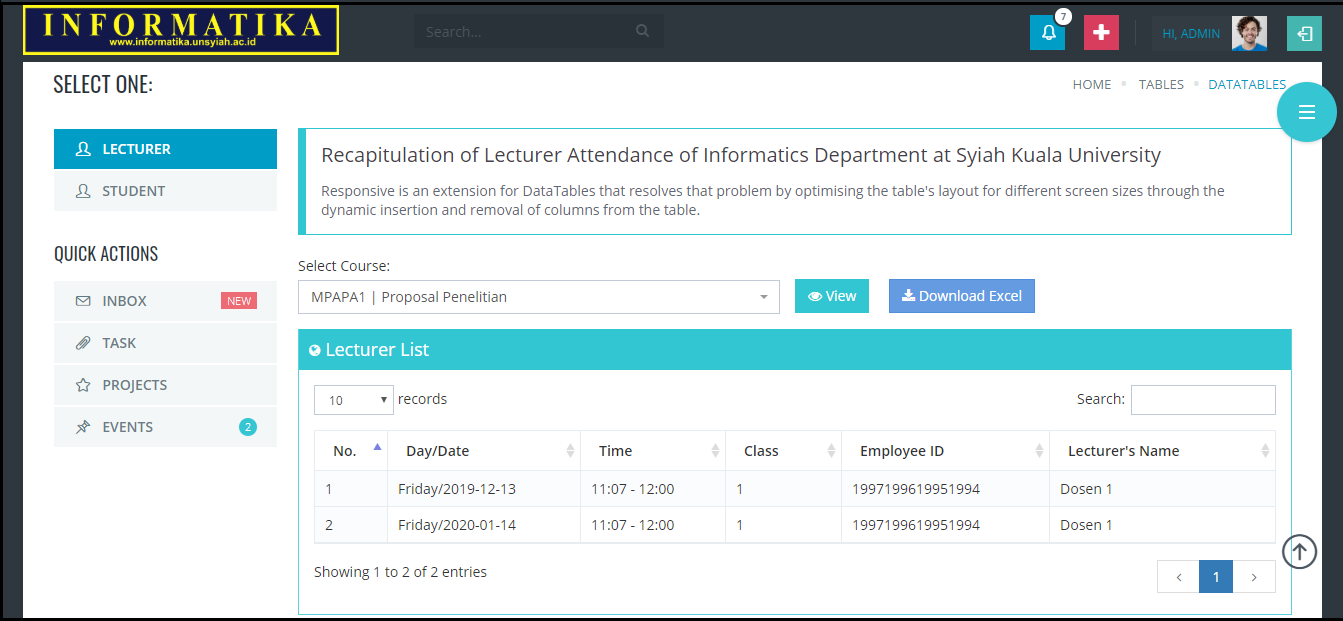
\includegraphics [width = 13cm, height= 6cm]{gambar/web/dashboard-dosen}
		\caption{Halaman Daftar Kehadiran Dosen}
		\label{web-daftar-dosen}
		\end{figure}
		
		\vspace{-0.2cm}
		\begin{figure}[H]
		\center
		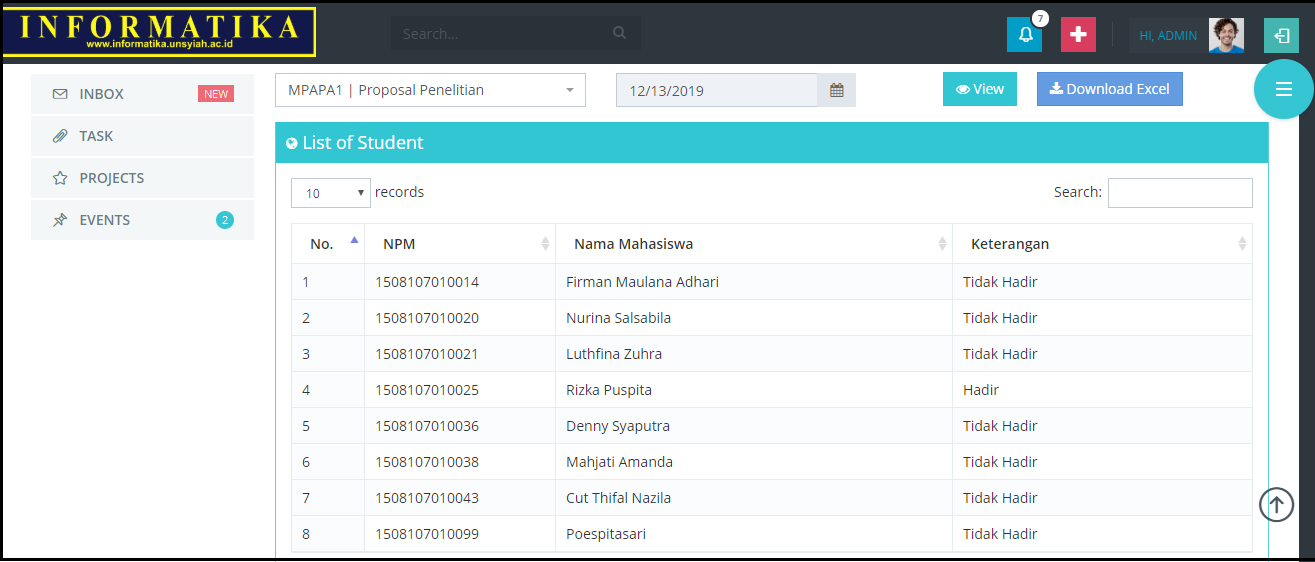
\includegraphics [width = 13cm, height= 6cm]{gambar/web/dashboard-mahasiswa}
		\caption{Halaman Daftar Kehadiran Mahasiswa}
		\label{web-daftar-mahasiswa}
		\end{figure}
		
		\vspace{-0.2cm}
		\begin{figure}[H]
		\center
		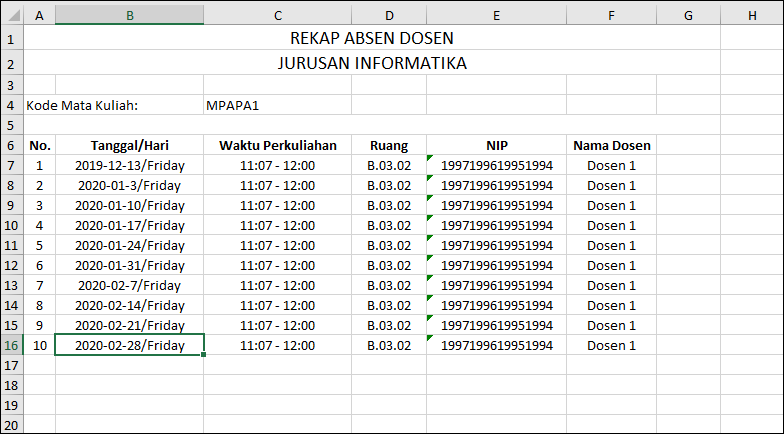
\includegraphics [width = 11cm, height= 6.3cm]{gambar/web/rekap-dosen}
		\caption{File Unduhan CSV Rekap Kehadiran Dosen}
		\label{web-csv-dosen}
		\end{figure}
		
		\vspace{-0.2cm}
		\begin{figure}[H]
		\center
		\includegraphics [width = 11cm, height= 6.3cm]{gambar/web/rekap-mahasiswa}
		\caption{File Unduhan CSV Rekap Kehadiran Mahasiswa}
		\label{web-csv-mahasiswa}
		\end{figure}
	
	\end{enumerate}
	
	\section{\uppercase{PENGUJIAN SISTEM}}
	\par Pengujian sistem dilakukan untuk melihat apakah sistem dapat berjalan dengan tepat sesuai dengan rancangan. Beberapa pengujian yang dilakukan pada penelitian ini adalah pengujian keakuratan klasifikasi menggunakan metode klasifikasi K-NN, pengujian usabilitas dengan metode SUS dan pengujian fungsionalitas menggunakan \textit{Blackbox}. 
		
\subsection{Pengujian Keakuratan Klasifikasi Menggunakan Metode Klasifikasi K-NN}
\begin{enumerate}

\item Pengujian Keakuratan Klasifikasi Reference Point

\par Pengujian ini dianalisis menggunakan metode klasifikasi K-NN. Pengujian ini bertujuan untuk menganalisis jenis penyebaran \textit{reference point} yang terbaik dengan membandingkan \textit{F-Measure} yang didapatkan dari setiap pengujian. Data \textit{training} yang digunakan pada penelitian ini sebanyak 764 data kekuatan sinyal dengan masing-masing 324 data kekuatan sinyal untuk \textit{reference point} acak, 440 data kekuatan sinyal untuk \textit{reference point} urut dan 160 sebagai data uji. Pengumpulan data \textit{training} dilakukan dengan cara melakukan pemetaan kekuataan sinyal yang telah dijelaskan pada \textbf{BAB III}. Hasil dari proses pengujian metode klasifikasi K-NN menunjukkan bahwa dengan K=5 untuk data kekuatan sinyal \textit{reference point} urut, memiliki rata-rata \textit{F-Measure} paling baik dengan nilai 78,60\% dibandingkan dengan parameter pengujian lainnya. Hasil pengujian menggunakan metode K-NN ini  dapat dilihat pada Tabel \ref{tabelfmeasure9}.
% Please add the following required packages to your document preamble:
% \usepackage{multirow}
\begin{table}[H]
\fontsize{9}{12}\selectfont
\center
\caption{Perbandingan F-Measure}
\label{tabelfmeasure9}
\begin{tabular}{|c|c|l|c|c|c|c|}
\hline
Jenis Titik           & Nilai K            & \multicolumn{1}{c|}{Kelas Label} & Precision & Recall  & F-Measure & Rata-Rata F-Measure      \\ \hline
\multirow{3}{*}{Urut} & \multirow{3}{*}{3} & B0302                            & 90,69\%   & 66,10\% & 76,47\%   & \multirow{3}{*}{78,52\%} \\ \cline{3-6}
                      &                    & E0207                            & 82,60\%   & 70,37\% & 76,00\%    &                          \\ \cline{3-6}
                      &                    & Luar Kelas                       & 83,09\%   & 83,09\% & 83,09\%   &                          \\ \hline
\multirow{3}{*}{Urut} & \multirow{3}{*}{5} & B0302                            & 90,69\%   & 66,10\% & 76,47\%   & \multirow{3}{*}{78,60\%} \\ \cline{3-6}
                      &                    & E0207                            & 81,25\%   & 72,22\% & 76,47\%   &                          \\ \cline{3-6}
                      &                    & Luar Kelas                       & 84,05\%   & 81,69\% & 82,85\%   &                          \\ \hline
\multirow{3}{*}{Urut} & \multirow{3}{*}{7} & B0302                            & 90,69\%   & 67,24\% & 72,20\%   & \multirow{3}{*}{77,42\%} \\ \cline{3-6}
                      &                    & E0207                            & 81,63\%   & 74,07\% & 76,60\%   &                          \\ \cline{3-6}
                      &                    & Luar Kelas                       & 85,29\%   & 81,69\% & 83,45\%   &                          \\ \hline
\multirow{3}{*}{Acak} & \multirow{3}{*}{3} & B0302                            & 97,36\%   & 60,65\% & 74,74\%   & \multirow{3}{*}{77,66\%} \\ \cline{3-6}
                      &                    & E0207                            & 78,00\%   & 73,58\% & 75,72\%   &                          \\ \cline{3-6}
                      &                    & Luar Kelas                       & 81,94\%   & 83,09\% & 82,51\%   &                          \\ \hline
\multirow{3}{*}{Acak} & \multirow{3}{*}{5} & B0302                            & 97,43\%   & 59,37\% & 73,78\%   & \multirow{3}{*}{76,07\%} \\ \cline{3-6}
                      &                    & E0207                            & 75,51\%   & 71,15\% & 73,26\%   &                          \\ \cline{3-6}
                      &                    & Luar Kelas                       & 80,55\%   & 81,69\% & 81,18\%   &                          \\ \hline
\multirow{3}{*}{Acak} & \multirow{3}{*}{7} & B0302                            & 97,36\%   & 59,67\% & 74,00\%    & \multirow{3}{*}{76,89\%} \\ \cline{3-6}
                      &                    & E0207                            & 76,47\%   & 73,58\% & 74,99\%   &                          \\ \cline{3-6}
                      &                    & Luar Kelas                       & 81,69\%   & 81,69\% & 81,69\%   &                          \\ \hline
\end{tabular}
\end{table}


\par Ilustrasi dari perbandingan F-Measure setiap parameter pengujian ditampilkan pada Gambar \ref{gambar-grafik-akurasi-klasifikasi-9-beacon}.
		\begin{figure}[H]
			\center
			\shadowbox
			{\includegraphics [width = 13cm, height= 7cm]{gambar/pengujian/grafik-akurasi-klasifikasi}}
			\caption{Grafik Perbandingan F-Measure dengan Menggunakan Parameter Pengujian yang Berbeda.}
			\label{gambar-grafik-akurasi-klasifikasi-9-beacon}
		\end{figure}
		
		\vspace{2cm}
		\par Pengambilan data uji dilakukan untuk menguji tingkat keberhasilan klasifikasi dengan melihat akurasi tertinggi bergantung pada parameter nilai K yang digunakan. Pada pengujian ini terdapat titik yang sering salah diprediksi yaitu sebanyak 6 dari 6 kali pengujian. Lokasi titik yang sering salah diprediksi ditandai dengan lingkaran bewarna biru yang ditampilkan dalam bentuk ilustrasi denah yang dapat dilihat pada Gambar \ref{gambar-denah-titik-uji-b0302} dan Gambar \ref{gambar-denah-titik-uji-e0207}.
\vspace{0.2cm}
		\begin{figure}[H]
			\center
			\includegraphics [width = 11cm, height= 9cm]{gambar/denah/B0302-Uji}
			\caption{Lokasi Titik yang Sering Salah Diprediksi di Kelas B.03.02.}
			\label{gambar-denah-titik-uji-b0302}
		\end{figure}
		
		\begin{figure}[H]
			\center
			\includegraphics [width = 14cm, height= 8cm]{gambar/denah/E0207-Uji}
			\caption{Lokasi Titik yang Sering Salah Diprediksi di Kelas E.02.07.}
			\label{gambar-denah-titik-uji-e0207}
		\end{figure}
%batas batas batas batas batas batas batas batas batas batas batas batas batas

\item Pengujian Keakuratan Reference Point Berdasarkan Penggunaan Jumlah Beacon pada Ruang Kuliah B.03.02

\par Pengujian ini dianalisis menggunakan metode klasifikasi K-NN. Pengujian ini bertujuan untuk menganalisis tingkat keakuratan klasifikasi jenis \textit{reference point} terbaik yang digunakan dengan membandingkan penggunaan jumlah Beacon dengan melihat \textit{F-Measure} yang didapatkan dari setiap pengujian. Jumlah Beacon yang dibandingkan adalah 3 Beacon dan 6 Beacon. Data \textit{training} yang digunakan pada penelitian ini sebanyak 368 data kekuatan sinyal dengan masing-masing 120 data kekuatan sinyal untuk \textit{reference point} acak, 168 data kekuatan sinyal untuk \textit{reference point} urut dan 80 sebagai data uji. Pengumpulan data \textit{training} dilakukan dengan cara melakukan pemetaan kekuataan sinyal yang telah dijelaskan pada \textbf{BAB III}. Hasil dari proses pengujian metode klasifikasi K-NN menunjukkan bahwa dengan K=5 untuk data kekuatan sinyal \textit{reference point} acak menggunakan 6 Beacon, memiliki \textit{F-Measure} paling baik dengan nilai 96,20\% dibandingkan dengan parameter pengujian lainnya. Hasil pengujian menggunakan metode K-NN ini dapat dilihat secara detil pada Tabel \ref{tabelfmeasureee}.
% Please add the following required packages to your document preamble:
% \usepackage{multirow}
\begin{table}[H]
\fontsize{10}{12}\selectfont
\center
\caption{Perbandingan F-Measure}
\label{tabelfmeasureee}
\begin{tabular}{|c|c|l|c|c|c|}
\hline
Nilai K            & Jumlah BLE         & \multicolumn{1}{c|}{Jenis Titik} & Precision & Recall  & F-Measure \\ \hline
\multirow{2}{*}{3} & \multirow{2}{*}{3} & Urut                             & 67,24\%   & 97,50\% & 80,00\%    \\ \cline{3-6} 
                   &                    & Acak                             & 82,50\%   & 82,50\% & 82,50\%   \\ \hline
\multirow{2}{*}{5} & \multirow{2}{*}{3} & Urut                             & 67,24\%   & 97,50\% & 80,00\%    \\ \cline{3-6} 
                   &                    & Acak                             & 80,50\%   & 82,50\% & 81,50\%   \\ \hline
\multirow{2}{*}{7} & \multirow{2}{*}{3} & Urut                             & 67,24\%   & 97,50\% & 80,00\%    \\ \cline{3-6} 
                   &                    & Acak                             & 80,50\%   & 82,50\% & 81,50\%   \\ \hline
\multirow{2}{*}{3} & \multirow{2}{*}{6} & Urut                             & 90,70\%   & 97,50\% & 94,00\%    \\ \cline{3-6} 
                   &                    & Acak                             & 97,40\%   & 92,50\% & 95,00\%    \\ \hline
\multirow{2}{*}{5} & \multirow{2}{*}{6} & Urut                             & 90,70\%   & 97,50\% & 94,00\%    \\ \cline{3-6} 
                   &                    & Acak                             & 97,40\%   & 95,00\%  & 96,20\%   \\ \hline
\multirow{2}{*}{7} & \multirow{2}{*}{6} & Urut                             & 90,70\%   & 97,50\% & 94,00\%    \\ \cline{3-6} 
                   &                    & Acak                             & 97,40\%   & 92,50\% & 95,00\%    \\ \hline
\end{tabular}
\end{table}

\par Ilustrasi dari perbandingan F-Measure setiap parameter pengujian ditampilkan pada Gambar \ref{gambar-grafik-akurasi-klasifikasi-6-beacon}.
		\begin{figure}[H]
			\center
			\shadowbox
			{\includegraphics [width = 14cm, height= 8.7cm]{gambar/pengujian/grafik-akurasi-klasifikasi-kelas-b0302}}
			\caption{Grafik Perbandingan F-Measure dengan Menggunakan Parameter Pengujian yang Berbeda.}
			\label{gambar-grafik-akurasi-klasifikasi-6-beacon}
		\end{figure}
		
\par Berdasarkan hasil pengujian dengan parameter nilai K yang berbeda menggunakan 3 Beacon dan 6 Beacon berdasarkan jenis \textit{reference point} yang digunakan, menunjukkan bahwa penggunaan 6 Beacon mengurangi kesalahan prediksi titik dibandingkan dengan 3 Beacon. Ilustrasi perbandingan tersebut dapat ditampilkan pada Gambar \ref{gambar-grafik-titik-salah-prediksi}.	
		\begin{figure}[H]
			\center
			\shadowbox
			{\includegraphics [width = 9cm, height= 5cm]{gambar/pengujian/grafik-titik-salah-prediksi}}
			\caption{Grafik Jumlah Titik yang Salah Diprediksi.}
			\label{gambar-grafik-titik-salah-prediksi}
		\end{figure}
		

%batas batas batas batas batas batas batas batas batas batas batas batas batas	
\end{enumerate} 

\subsection{Pengujian Usabilitas Menggunakan Metode SUS}
\par Pengujian usabilitas bertujuan untuk menguji kelayakan dan kegunaan dari sistem yang akan digunakan oleh pengguna. Sebelum melakukan pengujian ini, adapun \textit{Test Plan} yang telah dibuat untuk yang dapat dilihat pada Tabel \ref{testplan-aplikasi-dosen} dan Tabel \ref{testplan-aplikasi-mahasiswa}.

\begin{table}[H]
\fontsize{10}{12}\selectfont
\center
\caption{\textit{Test Plan} Aplikasi Kehadiran Dosen}
\label{testplan-aplikasi-dosen}
\begin{tabular}{|l|l|l|l|l|}
\hline
\multicolumn{5}{|c|}{\textbf{Test Plan Aplikasi Kehadiran Dosen}}                                                                                                                                                                                                          \\ \hline
\multicolumn{5}{|l|}{\begin{tabular}[c]{@{}l@{}}Lokasi:\\ Ruang kuliah B.03.02 \\Ruang Kuliah E.03.07\end{tabular}}                                                                                                                                                                               \\ \hline
\multicolumn{5}{|l|}{\begin{tabular}[c]{@{}l@{}}Skenario:\\ 1. Dosen melakukan \textit{log in} ke aplikasi.\\ 2. Dosen memahami tampilan halaman beranda. \\ 3. Dosen melihat daftar mahasiswa yang mengambil suatu mata kuliah. \\ 4. Dosen memulai proses kehadiran.\\ 5. Dosen melihat hasil prediksi lokasi yang dilakukan oleh aplikasi.\end{tabular}} \\ \hline
\multicolumn{5}{|l|}{\begin{tabular}[c]{@{}l@{}}Alat:\\ 1. Smartphone Android\\ 2. Beacon\end{tabular}}                                                                                                                                                                    \\ \hline
\multicolumn{5}{|l|}{\begin{tabular}[c]{@{}l@{}}Hasil:\\ Hasil pengujian dapat dilihat pada tabel dan lampiran.\end{tabular}}                                                                                                                                              \\ \hline
\end{tabular}
\end{table}

\begin{table}[H]
\fontsize{10}{12}\selectfont
\center
\caption{\textit{Test Plan} Aplikasi Kehadiran Mahasiswa}
\label{testplan-aplikasi-mahasiswa}
\begin{tabular}{|l|l|l|l|l|}
\hline
\multicolumn{5}{|c|}{\textbf{Test Plan Aplikasi Kehadiran Mahasiswa}}                                                                                                                                                                                                                                                                             \\ \hline
\multicolumn{5}{|l|}{\begin{tabular}[c]{@{}l@{}}Lokasi:\\ Ruang kuliah B.03.02 \\Ruang Kuliah E.03.07\end{tabular}}                                                                                                                                                                                                                                                      \\ \hline
\multicolumn{5}{|l|}{\begin{tabular}[c]{@{}l@{}}Skenario:\\ 1. Mahasiswa melakukan \textit{log in} ke aplikasi.\\ 2. Mahasiswa melihat halaman profil data diri.\\ 3. Mahasiswa melihat daftar mata kuliah yang diambil.\\ 4. Mahasiswa memulai proses kehadiran.\\ 5. Mahasiswa melihat hasil prediksi lokasi yang dilakukan oleh aplikasi.\end{tabular}} \\ \hline
\multicolumn{5}{|l|}{\begin{tabular}[c]{@{}l@{}}Alat:\\ 1. Smartphone Android\\ 2. Beacon\end{tabular}}                                                                                                                                                                                                                                           \\ \hline
\multicolumn{5}{|l|}{\begin{tabular}[c]{@{}l@{}}Hasil:\\ Hasil pengujian dapat dilihat pada tabel dan lampiran.\end{tabular}}                                                                                                                                                                                                                     \\ \hline
\end{tabular}
\end{table}

\par Pengujian dengan metode SUS dilakukan dengan memberikan kuisioner kepada responden. Kuisioner tersebut berisi 10 pertanyaan seperti yang telah dibahas pada. Pengujian Aplikasi Kehadiran Dosen memiliki responden berjumlah 5 orang sedangkan pengujian Aplikasi Kehadiran Mahasiswa memiliki responden berjumlah 9 orang. Hasil skor pengujian metode SUS yang dilakukan dapat dilihat pada Tabel \ref{sus-aplikasi-dosen} dan Tabel \ref{sus-aplikasi-mahasiswa} berikut. 
%TABEL SUS APLIKASI DOSEN%
\begin{table}[H]
\fontsize{10}{12}\selectfont
\center
\caption{Hasil Pengujian SUS Aplikasi Kehadiran Dosen}
\label{sus-aplikasi-dosen}
\begin{tabular}{|c|c|c|c|c|c|c|c|c|c|c|c|}
\hline
\multirow{2}{*}{\textbf{Responden}} & \multicolumn{10}{c|}{\textbf{Kode Pertanyaan}}                                                                                                                  & \multirow{2}{*}{\textbf{Skor SUS}} \\ \cline{2-11}
                                    & \textbf{R1} & \textbf{R2} & \textbf{R3} & \textbf{R4} & \textbf{R5} & \textbf{R6} & \textbf{R7} & \textbf{R8} & \textbf{R9} & \multicolumn{1}{l|}{\textbf{R10}} &                                    \\ \hline
1                                   & 3           & 2           & 4           & 1           & 4           & 4           & 4           & 3           & 4           & 2                                 & 67,5                               \\ \hline
2                                   & 5           & 2           & 5           & 4           & 4           & 2           & 4           & 2           & 4           & 5                                 & 67,5                               \\ \hline
3                                   & 4           & 2           & 4           & 1           & 4           & 2           & 4           & 1           & 4           & 4                                 & 75,0                                 \\ \hline
4                                   & 5           & 1           & 5           & 2           & 5           & 2           & 5           & 1           & 5           & 1                                 & 95,0                                 \\ \hline
5                                   & 5           & 2           & 5           & 1           & 4           & 2           & 5           & 2           & 5           & 2                                 & 87,5                               \\ \hline
\multicolumn{11}{|c|}{\textbf{Rata - Rata}}                                                                                                                                                           & \textbf{78,5}                      \\ \hline
\end{tabular}
\end{table}

%TABEL SUS APLIKASI MAHASISWA%
\begin{table}[H]
\fontsize{10}{12}\selectfont
\center
\caption{Hasil Pengujian SUS Aplikasi Kehadiran Mahasiswa}
\label{sus-aplikasi-mahasiswa}
\begin{tabular}{|c|c|c|c|c|c|c|c|c|c|c|c|}
\hline
\multirow{2}{*}{\textbf{Responden}} & \multicolumn{10}{c|}{\textbf{Kode Pertanyaan}}                                                                                                                  & \multirow{2}{*}{\textbf{Skor SUS}} \\ \cline{2-11}
                                    & \textbf{R1} & \textbf{R2} & \textbf{R3} & \textbf{R4} & \textbf{R5} & \textbf{R6} & \textbf{R7} & \textbf{R8} & \textbf{R9} & \multicolumn{1}{l|}{\textbf{R10}} &                                    \\ \hline
1                                   & 5           & 1           & 4           & 1           & 4           & 1           & 5           & 1           & 5           & 1                                 & 95,0                                 \\ \hline
2                                   & 5           & 2           & 4           & 2           & 4           & 2           & 4           & 2           & 2           & 2                                 & 72,5                               \\ \hline
3                                   & 5           & 2           & 5           & 2           & 5           & 1           & 5           & 1           & 5           & 2                                 & 92,5                               \\ \hline
4                                   & 5           & 1           & 5           & 1           & 5           & 1           & 5           & 1           & 5           & 1                                 & 100,0                                \\ \hline
5                                   & 5           & 1           & 5           & 2           & 5           & 1           & 5           & 1           & 5           & 2                                 & 95,0                                 \\ \hline
6                                   & 5           & 2           & 4           & 1           & 4           & 2           & 4           & 1           & 5           & 2                                 & 85,0                                 \\ \hline
7                                   & 5           & 3           & 4           & 2           & 4           & 2           & 4           & 2           & 3           & 5                                 & 65,0                                 \\ \hline
8                                   & 4           & 1           & 5           & 2           & 4           & 2           & 4           & 1           & 5           & 4                                 & 80,0                                 \\ \hline
9                                   & 5           & 1           & 5           & 2           & 5           & 2           & 5           & 2           & 5           & 2                                 & 90,0                                 \\ \hline
\multicolumn{11}{|c|}{\textbf{Rata - Rata}}                                                                                                                                                             & \textbf{86,1}                      \\ \hline
\end{tabular}
\end{table}

\par Berdasarkan hasil pengujian SUS yang telah dilakukan diatas, hasil rata-rata pengujian Aplikasi Kehadiran Dosen mendapatkan skor sebesar 78,5\% sedangkan hasil rata-rata pengujian Aplikasi Kehadiran Mahasiswa mendapatkan skor sebesar 86,1\%. Dapat dilihat bahwa kedua aplikasi yang telah dibangun memiliki skor interpretasi \textbf{"dapat diterima"} berdasarkan Tabel 3.4.  

\subsection{Pengujian Fungsionalitas Menggunakan Blackbox}
\par Pengujian \textit{Blackbox} dilakukan dengan tujuan untuk menguji fungsionalitas dari aplikasi dengan menjalankan aplikasi tersebut apakah sesuai dengan alur bisnis yang diinginkan. Pengujian ini melihat fungsi yang tidak sesuai pada aplikasi dan kesalahan-kesalahan aplikasi dalam mengerjakan suatu perintah. Pengujian ini dilakukan pada Aplikasi Mapping, Aplikasi Kehadiran Dosen, Aplikasi Kehadiran Mahasiswa, dan Aplikasi Web Rekap Kehadiran Dosen dan Mahasiswa. Beberapa fitur aplikasi yang diuji menggunakan \textit{Blackbox Testing} dapat dilihat pada Tabel \ref{blackbox-aplikasi-mapping}, Tabel \ref{blackbox-aplikasi-dosen}, Tabel \ref{blackbox-aplikasi-mahasiswa}, dan Tabel \ref{blackbox-web-admin}.
%TABEL APLIKASI MAPPING%
\begin{table}[H]
\fontsize{10}{12}\selectfont
\center
\caption{Pengujian \textit{Blackbox} Aplikasi Mapping}
\label{blackbox-aplikasi-mapping}
\begin{tabular}{|c|l|l|l|c|}
\hline
\textbf{No.} & \multicolumn{1}{c|}{\textbf{Nama Pengujian}}                                       & \multicolumn{1}{c|}{\textbf{Skenario}}                                                                                        & \multicolumn{1}{c|}{\textbf{Tampilan}}                                                                    & \textbf{Hasil}                \\ \hline
1.           & \begin{tabular}[c]{@{}l@{}}Menghidupkan \\ Bluetooth\end{tabular}                  & \begin{tabular}[c]{@{}l@{}}Klik tombol \textbf{Allow} \\ pada notifikasi yang\\ muncul\end{tabular}                                  & \begin{tabular}[c]{@{}l@{}}Bluetooth akan \\ hidup\end{tabular}                                           & Berhasil                      \\ \hline
2.           & \begin{tabular}[c]{@{}l@{}}Lakukan proses \\ pemindaian \\ sinyal BLE\end{tabular} & Klik tombol \textbf{"Scan"}                                                                                                            & \begin{tabular}[c]{@{}l@{}}Muncul nama BLE, \\ MAC Address BLE \\ dan kekuatan sinyal \\ BLE\end{tabular} & Berhasil                      \\ \hline
3.           & \begin{tabular}[c]{@{}l@{}}Menyimpan data \\ ke tabel titik acak\end{tabular}      & \begin{tabular}[c]{@{}l@{}}Mengisi nama ruang \\ kemudian klik tombol \\ \textbf{Save to} dan pilih \\ tabel titik acak\end{tabular} & \begin{tabular}[c]{@{}l@{}}Muncul \textit{pop up} \\ untuk memilih \\ tabel\end{tabular}                           & Berhasil                      \\ \hline
4.           & \begin{tabular}[c]{@{}l@{}}Menyimpan data \\ ke tabel titik urut\end{tabular}      & \begin{tabular}[c]{@{}l@{}}Mengisi nama ruang \\ kemudian klik tombol \\ \textbf{Save to} dan pilih \\ tabel titik urut\end{tabular} & \begin{tabular}[c]{@{}l@{}}Muncul \textit{pop up} \\ untuk memilih \\ tabel\end{tabular}                           & Berhasil                      \\ \hline
5.           & \begin{tabular}[c]{@{}l@{}}Melihat data \\ yang tersimpan\end{tabular}             & \begin{tabular}[c]{@{}l@{}}Klik tombol \\ \textbf{Show Data}\end{tabular}                                                            & \begin{tabular}[c]{@{}l@{}}Diarahkan ke \\ halaman daftar \\ data yang tersimpan\end{tabular}             & Berhasil                      \\ \hline
6.           & \begin{tabular}[c]{@{}l@{}}Menghapus data \\ yang tersimpan\end{tabular}           & \begin{tabular}[c]{@{}l@{}}Klik icon \textbf{Tong} \\ \textbf{Sampah}\end{tabular}                                                              & \begin{tabular}[c]{@{}l@{}}Muncul notifikasi \\ dan konfirmasi \\ untuk menghapus \\ data\end{tabular}    & \multicolumn{1}{l|}{Berhasil} \\ \hline
\end{tabular}
\end{table}

%BLACKBOX APLIKASI DOSEN%
\begin{table}[H]
\fontsize{10}{12}\selectfont
\center
\caption{Pengujian \textit{Blackbox } Aplikasi Kehadiran Dosen}
\label{blackbox-aplikasi-dosen}
\begin{tabular}{|c|l|l|l|c|}
\hline
No. & \multicolumn{1}{c|}{\textbf{Nama Pengujian}}                                                                              & \multicolumn{1}{c|}{\textbf{Skenario}}                                                                                    & \multicolumn{1}{c|}{\textbf{Tampilan}}                                                                                  & Hasil    \\ \hline
1.  & \begin{tabular}[c]{@{}l@{}}Melakukan \textit{log in} \\ ke aplikasi\end{tabular}                                          & \begin{tabular}[c]{@{}l@{}}Klik tombol \textbf{Submit} \\ setelah selesai \\ mengisi form \textit{log in}\end{tabular}             & \begin{tabular}[c]{@{}l@{}}Diarahkan ke \\ halaman beranda \\ aplikasi apabila \\ berhasil \textit{log in}\end{tabular} & Berhasil \\ \hline
2.  & \begin{tabular}[c]{@{}l@{}}Melihat informasi \\ suatu mata kuliah\end{tabular}                                   & \begin{tabular}[c]{@{}l@{}}Klik salah satu daftar \\ mata kuliah\end{tabular}                                    & \begin{tabular}[c]{@{}l@{}}Diarahkan ke \\ halaman informasi \\ mata kuliah\end{tabular}                       & Berhasil \\ \hline
3.  & \begin{tabular}[c]{@{}l@{}}Menghidupkan \\ Bluetooth\end{tabular}                                                & \begin{tabular}[c]{@{}l@{}}Klik tombol \textbf{Allow} \\ pada notifikasi yang \\ muncul\end{tabular}                      & \begin{tabular}[c]{@{}l@{}}Bluetooth akan \\ menyala\end{tabular}                                              & Berhasil \\ \hline
4.  & \begin{tabular}[c]{@{}l@{}}Melihat daftar \\ nama mahasiswa \\ yang mengambil  \\ suatu mata kuliah\end{tabular} & \begin{tabular}[c]{@{}l@{}}Klik tombol \\ \textbf{Show Students} pada \\ halaman informasi \\ mata kuliah\end{tabular}    & \begin{tabular}[c]{@{}l@{}}Diarahkan ke \\ halaman daftar \\ nama mahasiswa\end{tabular}                       & Berhasil \\ \hline
5.  & \begin{tabular}[c]{@{}l@{}}Memulai proses \\ kehadiran\end{tabular}                                              & \begin{tabular}[c]{@{}l@{}}Klik tombol \\ \textbf{Start Attendance} \\ pada halaman \\ informasi mata kuliah\end{tabular} & \begin{tabular}[c]{@{}l@{}}Secara \textit{background} \\ \textit{proccess} aplikasi \\ akan memproses \\ kehadiran\end{tabular}  & Berhasil \\ \hline
\end{tabular}
\end{table}

%BLACKBOX APLIKASI MAHASISWA%
\begin{table}[H]
\fontsize{10}{12}\selectfont
\center
\caption{Pengujian \textit{Blackbox} Aplikasi Kehadiran Mahasiswa}
\label{blackbox-aplikasi-mahasiswa}
\begin{tabular}{|c|l|l|l|c|}
\hline
No. & \multicolumn{1}{c|}{\textbf{Nama Pengujian}}                                                   & \multicolumn{1}{c|}{\textbf{Skenario}}                                                                                    & \multicolumn{1}{c|}{\textbf{Tampilan}}                                                                                  & Hasil                         \\ \hline
1.  & \begin{tabular}[c]{@{}l@{}}Melakukan \textit{log in}\\ ke aplikasi\end{tabular}                & \begin{tabular}[c]{@{}l@{}}Klik tombol \textbf{Submit} \\ setelah selesai \\ mengisi form \textit{log in}\end{tabular}             & \begin{tabular}[c]{@{}l@{}}Diarahkan ke \\ halaman beranda \\ aplikasi apabila \\ berhasil \textit{log in}\end{tabular} & Berhasil                      \\ \hline
2.  & \begin{tabular}[c]{@{}l@{}}Melihat daftar \\ mata kuliah \\ yang diambil\end{tabular} & Klik icon \textbf{My Course}                                                                                              & \begin{tabular}[c]{@{}l@{}}Diarahkan ke \\ halaman daftar \\ mata kuliah\end{tabular}                          & Berhasil                      \\ \hline
3.  & \begin{tabular}[c]{@{}l@{}}Melihat profil \\ data diri\end{tabular}                   & Klik icon \textbf{My Profile                                                                                            } & \begin{tabular}[c]{@{}l@{}}Diarahkan ke \\ halaman profil\end{tabular}                                         & \multicolumn{1}{l|}{Berhasil} \\ \hline
4.  & \begin{tabular}[c]{@{}l@{}}Menghidupkan \\ Bluetooth\end{tabular}                     & \begin{tabular}[c]{@{}l@{}}Klik tombol \textbf{Allow} \\ pada notifikasi \\ yang muncul\end{tabular}                      & \begin{tabular}[c]{@{}l@{}}Bluetooth akan \\ menyala\end{tabular}                                              & Berhasil                      \\ \hline
5.  & \begin{tabular}[c]{@{}l@{}}Memulai \\ proses kehadiran\end{tabular}                   & \begin{tabular}[c]{@{}l@{}}Klik tombol \\ \textbf{Start Attendance} \\ pada salah satu \\ daftar mata kuliah\end{tabular} & \begin{tabular}[c]{@{}l@{}}Secara \textit{background} \\ \textit{proccess} aplikasi \\ akan memproses \\ kehadiran\end{tabular}  & Berhasil                      \\ \hline
\end{tabular}
\end{table}

%BLACKBOX WEB ADMIN%
\begin{table}[H]
\fontsize{10}{12}\selectfont
\center
\caption{Pengujian \textit{Blackbox} Aplikasi Web Rekap Kehadiran Dosen dan Mahasiswa}
\label{blackbox-web-admin}
\begin{tabular}{|c|l|l|l|c|}
\hline
No. & \multicolumn{1}{c|}{\textbf{Nama Pengujian}}                                                   & \multicolumn{1}{c|}{\textbf{Skenario}}                                                                                    & \multicolumn{1}{c|}{\textbf{Tampilan}}                                                                                  & Hasil                         \\ \hline
1.  & \begin{tabular}[c]{@{}l@{}}Melakukan \textit{log in}\\ ke aplikasi\end{tabular}                & \begin{tabular}[c]{@{}l@{}}Klik tombol \\ \textbf{Submit} setelah \\ selesai mengisi \\ form \textit{log in}\end{tabular}          & \begin{tabular}[c]{@{}l@{}}Diarahkan ke \\ halaman beranda \\ aplikasi apabila \\ berhasil \textit{log in}\end{tabular} & Berhasil                      \\ \hline
2.  & \begin{tabular}[c]{@{}l@{}}Melihat daftar \\ mata kuliah \\ yang diambil\end{tabular} & \begin{tabular}[c]{@{}l@{}}Klik icon \\ \textbf{My Course}\end{tabular}                                                   & \begin{tabular}[c]{@{}l@{}}Diarahkan ke \\ halaman daftar \\ mata kuliah\end{tabular}                          & Berhasil                      \\ \hline
3.  & \begin{tabular}[c]{@{}l@{}}Melihat profil \\ data diri\end{tabular}                   & \begin{tabular}[c]{@{}l@{}}Klik icon \\ \textbf{My Profile}\end{tabular}                                                  & \begin{tabular}[c]{@{}l@{}}Diarahkan ke \\ halaman profil\end{tabular}                                         & \multicolumn{1}{l|}{Berhasil} \\ \hline
4.  & \begin{tabular}[c]{@{}l@{}}Menghidupkan \\ Bluetooth\end{tabular}                     & \begin{tabular}[c]{@{}l@{}}Klik tombol \\ \textbf{Allow} pada \\ notifikasi yang\\ muncul\end{tabular}                    & \begin{tabular}[c]{@{}l@{}}Bluetooth akan \\ menyala\end{tabular}                                              & Berhasil                      \\ \hline
5.  & \begin{tabular}[c]{@{}l@{}}Memulai \\ proses kehadiran\end{tabular}                   & \begin{tabular}[c]{@{}l@{}}Klik tombol \\ \textbf{Start Attendance} \\ pada salah satu \\ daftar mata kuliah\end{tabular} & \begin{tabular}[c]{@{}l@{}}Secara \textit{background} \\ \textit{proccess} aplikasi \\ akan memproses \\ kehadiran\end{tabular}  & Berhasil                      \\ \hline
\end{tabular}
\end{table}

%AKHIR DARI TABEL%
\par Berdasarkan hasil \textit{Blackbox Testing} dari tabel diatas menunjukkan bahwa Aplikasi Mapping, Aplikasi Kehadiran Dosen, Aplikasi Kehadiran Mahasiswa, dan Aplikasi Web Rekap Kehadiran Dosen dan Mahasiswa dapat berjalan dengan baik dibuktikan dengan  \textbf{"berhasil"} pada kolom hasil pengujian masing-masing fitur yang dikerjakan.


\begin{comment}
\bibliography{daftar-pustaka}
\end{comment}

	%-------------------------------------------------------------------------------
%                            	BAB V
%               		KESIMPULAN DAN SARAN
%-------------------------------------------------------------------------------
\fancyhf{} 
\fancyfoot[C]{\thepage}
\chapter{KESIMPULAN DAN SARAN}

\section{\uppercase{KESIMPULAN}}
	Berdasarkan penelitian yang telah dilakukan, dapat diambil kesimpulan bahwa:
	\begin{enumerate}
		\item \textit{Indoor Positioning System} telah berhasil diimplementasikan dengan menggunakan metode klasifikasi K-NN untuk memprediksi lokasi pengguna di dalam ruangan atau gedung (\textit{indoor}).
		\item Metode klasifikasi K-NN dengan parameter pengujian nilai K=5 untuk data kekuatan sinyal pada jenis \textit{reference point} urut, memiliki \textit{F-Measure} paling baik dibandingkan dengan parameter pengujian lainnya dengan nilai 78,60\%.
		\item Berdasarkan hasil pengujian akurasi klasifikasi dengan metode K-NN menggunakan 6 Beacon dengan parameter pengujian nilai K=5 untuk jenis \textit{referencen point} acak, memiliki F-Measure paling baik dengan nilai 96,2\% dibandingkan dengan menggunakan 3 Beacon.
		\item Berdasarkan hasil pengujian usabilitas menggunakan metode SUS, Aplikasi Kehadiran Dosen dan Aplikasi Kehadiran Mahasiswa dapat diterima dan mudah digunakan dilihat dari tingkat pemahaman pengguna.
		\item Berdasarkan hasil pengujian fungsionalitas menggunakan \textit{Black Box}, Aplikasi Kehadiran Dosen dan Aplikasi Kehadiran Mahasiswa telah berjalan sesuai dengan alur bisnis.
	\end{enumerate}



\section{\uppercase{SARAN}}

	Penelitian ini masih banyak kekurangan sehingga perlu dikembangkan agar menjadi lebih baik. Berikut adalah saran untuk penelitian ini:
	\begin{enumerate}
		\item Tampilan dari aplikasi berbasis Android dibuat lebih \textit{user-friendly}.
		\item Menambahkan fitur-fitur yang lebih banyak lagi pada Aplikasi Kehadiran Dosen seperti: dapat menghapus mahasiswa yang tidak benar-benar berada di dalam ruang kuliah dan memberhentikan proses pencatatan kehadiran saat materi kuliah sudah habis (sebelum jam mata kuliah berakhir).
		\item Aplikasi Kehadiran Dosen dan Aplikasi Kehadiran Mahasiswa hanya bisa berjalan pada \textit{smartphone} Android versi diatas 8.0 dikarenakan menggunakan \textit{Foreground Service} bawaan Android. Sebaiknya ditemukan metode yang lebih baik lagi agar kedua aplikasi tersebut bisa berjalan pada \textit{smartphone} Android versi dibawah 8.0.
		\item Aplikasi Kehadiran Dosen dan Aplikasi Kehadiran Mahasiswa baiknya dibangun juga  versi iOS.
		\item Mencari metode klasifikasi atau metode penentuan lokasi yang lebih baik lagi untuk memprediksi lokasi pengguna.
		\item Sebaiknya ditambahkan lagi jumlah Beacon disetiap ruangan supaya meningkatkan keakuratan klasifikasi.
		\item Pengoptimisasian algoritma perhitungan jarak juga dibutuhkan, guna mengurangi waktu komputasi saat melakukan proses absen apabila kelas yang digunakan sudah sangat banyak.
	\end{enumerate}

\fancyhf{} 
\fancyfoot[R]{\thepage}
% Baris ini digunakan untuk membantu dalam melakukan sitasi
% Karena diapit dengan comment, maka baris ini akan diabaikan
% oleh compiler LaTeX.

\begin{comment}
\bibliography{daftar-pustaka}
\end{comment}


	\begin{spacing}{1}
		\bibliography{daftar-pustaka}
	\end{spacing}
	\addcontentsline{toc}{chapter}{DAFTAR KEPUSTAKAAN}
	%-----------------------------------------------------------------
	% Disini akhir masukan Daftar Pustaka
	%-----------------------------------------------------------------

	%%
% @author Kurnia Saputra
% @version 1.0
% 
% Hanya sebuah pembatas bertuliskan LAMPIRAN ditengah halaman. 
% 

\begin{titlepage}
	\centering 
	\vspace*{6cm}
	\noindent \Huge{LAMPIRAN}
	%\addChapter{LAMPIRAN}
	\addcontentsline{toc}{chapter}{LAMPIRAN}
\end{titlepage}
	%-----------------------------------------------------------------------------%
\addcontentsline{toc}{chapter}{LAMPIRAN 1}
\chapter*{Lampiran 1}
\newappendix{Lampiran 1. Sertifikat HKI Aplikasi Mapping}	
\begin{figure}[H]
\centering
\includegraphics[width = 14cm, height = 21cm]{gambar/lampiran/sertifikat}
\end{figure}
				
%------------------------------------------------------%
\addcontentsline{toc}{chapter}{LAMPIRAN 2}
\chapter*{Lampiran 2}
\newappendix{Lampiran 2. Foto Pengujian Usability}
\begin{figure}[htp]
\centering
\includegraphics[width=.3\textwidth]{gambar/lampiran/bu_viska_sus.jpg}\quad
\includegraphics[width=.3\textwidth]{gambar/lampiran/pak_rahmad_sus.jpg}\quad
\includegraphics[width=.3\textwidth]{gambar/lampiran/pak_yan_sus.jpg}

\medskip

\includegraphics[width=.3\textwidth]{gambar/lampiran/pak_kur_sus.jpg}\quad
\includegraphics[width=.3\textwidth]{gambar/lampiran/pak_taufik_sus.jpg}

\label{sus-dosen}
\end{figure}


\vspace{2cm}

\begin{figure}[htp]
\centering
\includegraphics[width=.3\textwidth]{gambar/lampiran/firman_sus.jpg}\quad
\includegraphics[width=.3\textwidth]{gambar/lampiran/ariq_sus.jpg}\quad
\includegraphics[width=.3\textwidth]{gambar/lampiran/safrul_sus.jpg}

\medskip

\includegraphics[width=.3\textwidth]{gambar/lampiran/lia_sus.jpg}\quad
\includegraphics[width=.3\textwidth]{gambar/lampiran/anis_sus.jpg}

\label{sus-mahasiswa}
\end{figure}


%-----------------------------------------------------------------------------%
%\addcontentsline{toc}{chapter}{LAMPIRAN 3}
%\chapter*{Lampiran 3}
%\newappendix{Lampiran 3. Foto Pengujian \textit{Usability}}

%-----------------------------------------------------------------------------%

%Lampiran 4 Laporan Usability

%\includepdf[pages=1,scale=.8,pagecommand={
%	\addcontentsline{toc}{chapter}{LAMPIRAN 4} 
%	\chapter*{Lampiran 4}
%	\newappendix{Lampiran 4. Laporan Hasil Pengujian \textit{Usability}}
%},linktodoc=true]{laporan_usability}
%\includepdf[pages=2-,scale=.8,pagecommand={},linktodoc=true]{laporan_usability}

	\addcontentsline{toc}{chapter}{LAMPIRAN} %daftar lampiran

\end{onehalfspace}

\end{document}